% !TeX spellcheck = da_DK
%implementing document formatting:
\documentclass[a4paper,11pt,fleqn,dvipsnames,oneside,openright,oldfontcommands]{memoir} 	% Openright aabner kapitler paa hoejresider (openany begge)


%%%%%%%%% Indsat random
%makes it possible to refer to the name of a chapter rather than just the number.
\usepackage{nameref}
\usepackage{pdfpages}
\usepackage{marvosym}
\usepackage{setspace}
\usepackage{graphicx} % For at sætte 2 billeder ved siden af hinanden

%package for writing program code in latex
\usepackage{listings}
%%%%%%%%%%%%%%%%%%%%%%

% ¤¤ Oversaettelse og tegnsaetning ¤¤ %
\usepackage[T1]{fontenc}					% Output-indkodning af tegnsaet (T1)
\usepackage[danish]{babel}					% Dokumentets sprog
\usepackage[utf8]{inputenc}					% Input-indkodning af tegnsaet (UTF8)
\usepackage{ragged2e,anyfontsize}			% Justering af elementer
\usepackage{fixltx2e}						% Retter forskellige fejl i LaTeX-kernen							
				
																							
% ¤¤ Figurer og tabeller (floats) ¤¤ %
\usepackage{graphicx} 						% Haandtering af eksterne billeder (JPG, PNG, EPS, PDF)
%\usepackage{eso-pic}						% Tilfoej billedekommandoer paa hver side
%\usepackage{wrapfig}						% Indsaettelse af figurer omsvoebt af tekst. \begin{wrapfigure}{Placering}{Stoerrelse}
\usepackage{multirow}                		% Fletning af raekker og kolonner (\multicolumn og \multirow)
\usepackage{multicol}         	        	% Muliggoer output i spalter
\usepackage{rotating}						% Rotation af tekst med \begin{sideways}...\end{sideways}
\usepackage{colortbl} 						% Farver i tabeller (fx \columncolor og \rowcolor)
\usepackage{xcolor}							% Definer farver med \definecolor. Se mere: http://en.wikibooks.org/wiki/LaTeX/Colors
\usepackage{flafter}						% Soerger for at floats ikke optraeder i teksten foer deres reference
\let\newfloat\relax 						% Justering mellem float-pakken og memoir
\usepackage{float}							% Muliggoer eksakt placering af floats, f.eks. \begin{figure}[H]
\usepackage{array,booktabs,xcolor,longtable} % kan lave \hdashline i tabellertabe
\usepackage{arydshln}
\usepackage{tabu}

	
	
% ¤¤ Matematik mm. ¤¤
\usepackage{amsmath , amsthm , amsfonts , amssymb, float, stmaryrd} 		% Avancerede matematik-udvidelser
%\usepackage{mathtools}						% Andre matematik- og tegnudvidelser
\usepackage{textcomp}                 		% Symbol-udvidelser (f.eks. promille-tegn med \textperthousand )
\usepackage{rsphrase}						% Kemi-pakke til RS-saetninger, f.eks. \rsphrase{R1}
\usepackage[version=3]{mhchem} 				% Kemi-pakke til flot og let notation af formler, f.eks. \ce{Fe2O3}
\usepackage{siunitx}						% Flot og konsistent praesentation af tal og enheder med \si{enhed} og \SI{tal}{enhed}
\sisetup{output-decimal-marker = {,}}		% Opsaetning af \SI (DE for komma som decimalseparator) 

% ¤¤ Referencer og kilder ¤¤ %
\usepackage[danish]{varioref}				% Muliggoer bl.a. krydshenvisninger med sidetal (\vref)
\usepackage[numbers]{natbib}				% Udvidelse med naturvidenskabelige citationsmodeller
%\usepackage{xr}							% Referencer til eksternt dokument med \externaldocument{<NAVN>}
%\usepackage{glossaries}					% Terminologi- eller symbolliste (se mere i Daleifs Latex-bog)
\usepackage{lastpage}					% Gør det mulig at refere til sidste side 

% ¤¤ Misc. ¤¤ %
\usepackage{listings}						% Placer kildekode i dokumentet med \begin{lstlisting}...\end{lstlisting}
\usepackage{lipsum}							% Dummy text \lipsum[..]
\usepackage[shortlabels]{enumitem}			% Muliggoer enkelt konfiguration af lister
\usepackage{pdfpages}						% Goer det muligt at inkludere pdf-dokumenter med kommandoen \includepdf[pages={x-y}]{fil.pdf}	
\pdfoptionpdfminorversion=6					% Muliggoer inkludering af pdf dokumenter, af version 1.6 og hoejere
\pretolerance=2500 							% Justering af afstand mellem ord (hoejt tal, mindre orddeling og mere luft mellem ord)


% Kommentarer og rettelser med \fxnote. Med 'final' i stedet for 'draft' udloeser hver note en error i den faerdige rapport.
\usepackage[footnote,draft,danish,silent,nomargin]{fixme}		


%%%% CUSTOM SETTINGS %%%%

% ¤¤ Marginer ¤¤ %
\setlrmarginsandblock{3.0cm}{2.5cm}{*}		% \setlrmarginsandblock{Indbinding}{Kant}{Ratio}
\setulmarginsandblock{2.5cm}{3.0cm}{*}		% \setulmarginsandblock{Top}{Bund}{Ratio}
\checkandfixthelayout 						% Oversaetter vaerdier til brug for andre pakker

%	¤¤ Afsnitsformatering ¤¤ %
\setlength{\parindent}{6mm}           		% Stoerrelse af indryk
\setlength{\parskip}{0mm}          			% Afstand mellem afsnit ved brug af double Enter
\linespread{1,1}							% Linie afstand



% ¤¤ Indholdsfortegnelse ¤¤ %
\setsecnumdepth{subsection}		 			% Dybden af nummerede overkrifter (part/chapter/section/subsection)
\maxsecnumdepth{subsection}					% Dokumentklassens graense for nummereringsdybde
\settocdepth{section} 					% Dybden af indholdsfortegnelsen

% ¤¤ Lister ¤¤ %
\setlist{
  topsep=0pt,								% Vertikal afstand mellem tekst og listen
  itemsep=-1ex,								% Vertikal afstand mellem items
} 

%hyperlinks in the tabel of contents - comment this out before the report is printed.
\usepackage{hyperref}
\hypersetup{
	bookmarks = true,  % Show 'bookmark'-frame in pdf.
	colorlinks = true, % True = colored links, False = framed links.
	citecolor = black,  % Link color for references.
	linkcolor = black,  % Link color in table of contents.
	urlcolor = black,   % Link color for extern URLs.
}

% ¤¤ Opsaetning af figur- og tabeltekst ¤¤ %
\usepackage{caption}
\usepackage{subcaption}
\captionnamefont{\small\bfseries\itshape}	% Opsaetning af tekstdelen ('Figur' eller 'Tabel')
\captiontitlefont{\small}					% Opsaetning af nummerering
\captiondelim{. }							% Seperator mellem nummerering og figurtekst
\hangcaption								% Venstrejusterer flere-liniers figurtekst under hinanden
%\captionwidth{0.9\textwidth}					% Bredden af figurteksten
\setlength{\belowcaptionskip}{0pt}			% Afstand under figurteksten
\captionsetup[figure]{labelfont={bf,it},font={it}} % sætter nummer til fed og kursis. Resten til fed + skriften er mindre end resten
\captionsetup[table]{labelfont={bf,it},font={it}} 


% ¤¤ Opsaetning af listings ¤¤ %

\definecolor{commentGreen}{RGB}{34,139,24}
\definecolor{stringPurple}{RGB}{208,76,239}

\lstset{language=Matlab,					% Sprog
	basicstyle=\ttfamily\scriptsize,		% Opsaetning af teksten
	keywords={for,if,while,else,elseif,		% Noegleord at fremhaeve
			  end,break,return,case,
			  switch,function},
	keywordstyle=\color{blue},				% Opsaetning af noegleord
	commentstyle=\color{commentGreen},		% Opsaetning af kommentarer
	stringstyle=\color{stringPurple},		% Opsaetning af strenge
	showstringspaces=false,					% Mellemrum i strenge enten vist eller blanke
	numbers=left, numberstyle=\tiny,		% Linjenumre
	extendedchars=true, 					% Tillader specielle karakterer
	columns=flexible,						% Kolonnejustering
	breaklines, breakatwhitespace=true,		% Bryd lange linjer
}

% ¤¤ Navngivning ¤¤ %
\addto\captionsdanish{
	\renewcommand\appendixname{Bilag}
	\renewcommand\contentsname{Indholdsfortegnelse}	
	\renewcommand\appendixpagename{Bilag}
	\renewcommand\appendixtocname{Bilag}
	\renewcommand\cftchaptername{\chaptername~}				% Skriver "Kapitel" foran kapitlerne i indholdsfortegnelsen
	\renewcommand\cftappendixname{\appendixname~}			% Skriver "Appendiks" foran appendiks i indholdsfortegnelsen
}

% ¤¤ Kapiteludssende ¤¤ %
\definecolor{numbercolor}{gray}{0.7}		% Definerer en farve til brug til kapiteludseende
\newif\ifchapternonum

\makechapterstyle{jenor}{					% Definerer kapiteludseende frem til ...
	\renewcommand\beforechapskip{0pt}
	\renewcommand\printchaptername{}
	\renewcommand\printchapternum{}
	\renewcommand\printchapternonum{\chapternonumtrue}
	\renewcommand\chaptitlefont{\fontfamily{pbk}\fontseries{db}\fontshape{n}\fontsize{20}{35}\selectfont\raggedright}
	\renewcommand\chapnumfont{\fontfamily{pbk}\fontseries{m}\fontshape{n}\fontsize{0.35in}{0in}\selectfont\color{black}}
	\renewcommand\printchaptertitle[1]{%
		\noindent
		\ifchapternonum
		\begin{tabularx}{\textwidth}{X}
			{\let\\\newline\chaptitlefont ##1\par} 
		\end{tabularx}
		\par\vskip-2.5mm\hrule
		\else
		\begin{tabularx}{\textwidth}{Xl}
			{\parbox[b]{\linewidth}{\chaptitlefont ##1}} & \raisebox{-5pt}{\chapnumfont \thechapter}
		\end{tabularx}
		\par\vskip2mm\hrule
		\fi
	}
}											% ... her

\chapterstyle{jenor}						% Valg af kapiteludseende - Google 'memoir chapter styles' for alternativer

% ¤¤ Sidehoved ¤¤ %

\makepagestyle{AAU}							% Definerer sidehoved og sidefod udseende frem til ...
\makepsmarks{AAU}{%
	\createmark{chapter}{left}{shownumber}{}{. \ }
	\createmark{section}{right}{shownumber}{}{. \ }
	\createplainmark{toc}{both}{\contentsname}
	\createplainmark{lof}{both}{\listfigurename}
	\createplainmark{lot}{both}{\listtablename}
	\createplainmark{bib}{both}{\bibname}
	\createplainmark{index}{both}{\indexname}
	\createplainmark{glossary}{both}{\glossaryname}
}
\nouppercaseheads											% Ingen Caps oenskes

\makeevenhead{AAU}{Gruppe 403}{}{\leftmark}				% Definerer lige siders sidehoved (\makeevenhead{Navn}{Venstre}{Center}{Hoejre})
\makeoddhead{AAU}{\rightmark}{}{Aalborg Universitet}		% Definerer ulige siders sidehoved (\makeoddhead{Navn}{Venstre}{Center}{Hoejre})
\makeevenfoot{AAU}{\thepage}{}{}							% Definerer lige siders sidefod (\makeevenfoot{Navn}{Venstre}{Center}{Hoejre})
\makeoddfoot{AAU}{}{}{\thepage}								% Definerer ulige siders sidefod (\makeoddfoot{Navn}{Venstre}{Center}{Hoejre})
\makeheadrule{AAU}{\textwidth}{0.5pt}						% Tilfoejer en streg under sidehovedets indhold
\makefootrule{AAU}{\textwidth}{0.5pt}{1mm}					% Tilfoejer en streg under sidefodens indhold

\copypagestyle{AAUchap}{AAU}								% Sidehoved for kapitelsider defineres som standardsider, men med blank sidehoved
\makeoddhead{AAUchap}{}{}{}
\makeevenhead{AAUchap}{}{}{}
\makeheadrule{AAUchap}{\textwidth}{0pt}
\aliaspagestyle{chapter}{AAUchap}							% Den ny style vaelges til at gaelde for chapters
% ... her

\pagestyle{AAU}												% Valg af sidehoved og sidefod


%%%% CUSTOM COMMANDS %%%%

% ¤¤ Billede hack ¤¤ %
\newcommand{\figur}[4]{
		\begin{figure}[H] \centering
			\includegraphics[width=#1\textwidth]{billeder/#2}
			\caption{#3}\label{#4}
		\end{figure} 
}

% ¤¤ Specielle tegn ¤¤ %
\newcommand{\decC}{^{\circ}\text{C}}
\newcommand{\dec}{^{\circ}}
\newcommand{\m}{\cdot}


%%%% ORDDELING %%%%

\hyphenation{}

%%%%Fra engelsk til dansk i \autoref{•} %%%%
\renewcommand{\figureautorefname}{Figur}
\renewcommand{\sectionautorefname}{Afsnit}
\renewcommand{\subsectionautorefname}{Afsnit}
\renewcommand{\subsubsectionautorefname}{Afsnit}
\renewcommand{\tableautorefname}{Tabel}
\renewcommand{\appendixautorefname}{Bilag}
\renewcommand{\equationautorefname}{Ligning}
\renewcommand{\itemautorefname}{Punkt}
\renewcommand{\chapterautorefname}{Kapitel}
%Figure references:
\newcommand{\figref}[1]{figur \ref{#1}}

%Figure references after full stop/period:
\newcommand{\Figref}[1]{Figur \ref{#1}}

%Table references:
\newcommand{\tabref}[1]{tabel \ref{#1}}

%Table references after full stop/period:
\newcommand{\Tabref}[1]{Tabel \ref{#1}}

%Appendix references:
\newcommand{\appref}[1]{appendix \ref{#1}}

%Appendix references after full stop/period:
\newcommand{\Appref}[1]{Appendix \ref{#1}}

%Section references:
\newcommand{\secref}[1]{afsnit \ref{#1}}

%Section references:
\newcommand{\Secref}[1]{Afsnit \ref{#1}}

%chapter references: 
\newcommand{\chapref}[1]{kapitel \ref{#1}}

%chapter references: 
\newcommand{\Chapref}[1]{Kapitel \ref{#1}}


%Units:
%inserting '\omit' before '{\put' prior ot final compile will fix allignment (and generate errors)
\newcommand{\unit}[1]{{\put(300,0){$\hfill\left[\: #1 \:\right]$}}}

%Text:
\newcommand{\tx}[1]{\text{#1}}

%Equation references:
%1 equation:
\renewcommand{\eqref}[1]{ligning (\ref{#1})}
%2 equations:
\newcommand{\eqrefTwo}[2]{ligning (\ref{#1}) og (\ref{#2})}
%3 equations:
\newcommand{\eqrefThree}[3]{ligning (\ref{#1}), (\ref{#2}) og (\ref{#3})}
%4 equations:
\newcommand{\eqrefFour}[4]{ligning (\ref{#1}), (\ref{#2}), (\ref{#3}) og (\ref{#4})}
%5 equations:
\newcommand{\eqrefFive}[5]{ligning (\ref{#1}), (\ref{#2}), (\ref{#3}), (\ref{#4}) og (\ref{#5})}


%Equation references after full stop/period:
%1 equation:
\renewcommand{\Eqref}[1]{Ligning (\ref{#1})}
%2 equations:
\newcommand{\EqrefTwo}[2]{Ligning (\ref{#1}) og (\ref{#2})}
%3 equations:
\newcommand{\EqrefThree}[3]{Ligning (\ref{#1}), (\ref{#2}) og (\ref{#3})}
%4 equations:
\newcommand{\EqrefFour}[4]{Ligning (\ref{#1}), (\ref{#2}), (\ref{#3}) og (\ref{#4})}
%5 equations:
\newcommand{\EqrefFive}[5]{Ligning (\ref{#1}), (\ref{#2}), (\ref{#3}), (\ref{#4}) og (\ref{#5})}
\begin{document}

%numbers the pages with Roman numeral - starts from "i":
\frontmatter
\clearpage
\thispagestyle{empty}

%\begin{figure}[H]
%	\raggedleft
%		
\includegraphics[width=0.2\textwidth]{figures/aaulogo-da.png}
%\end{figure}


%\vspace*{\fill} 
%\begin{center}	
%	\begin{Huge}
%		P3 Projektrapport - efterår 2015\\
%		\vspace{5 mm}
%		\textbf{System til detektering af kropsbalance}\\
%		\vspace{3 mm}
%		Gruppe 375
%	\end{Huge}
%\end{center}
%\vspace*{\fill}

\begin{center}
	\vspace*{\baselineskip}
	\rule{\textwidth}{1.6pt}\vspace*{-\baselineskip}\vspace*{2pt} % Thick horizontal line
	\rule{\textwidth}{0.4pt}\\[\baselineskip] % Thin horizontal line
	
	{\huge Aktivitetsmåler til forebyggelse\\\hspace*{2ex} af fysisk inaktivitet hos børn \\[0.5\baselineskip] \large Projektrapport 4. semester}\\[0.2\baselineskip] % Title
	
	\rule{\textwidth}{0.4pt}\vspace*{-\baselineskip}\vspace{3.2pt} % Thin horizontal line
	\rule{\textwidth}{1.6pt}\\[\baselineskip] % Thick horizontal line
	\vspace*{5\baselineskip}
	\begin{figure}[H]
		\centering
		\begin{minipage}[c]{1\textwidth}
			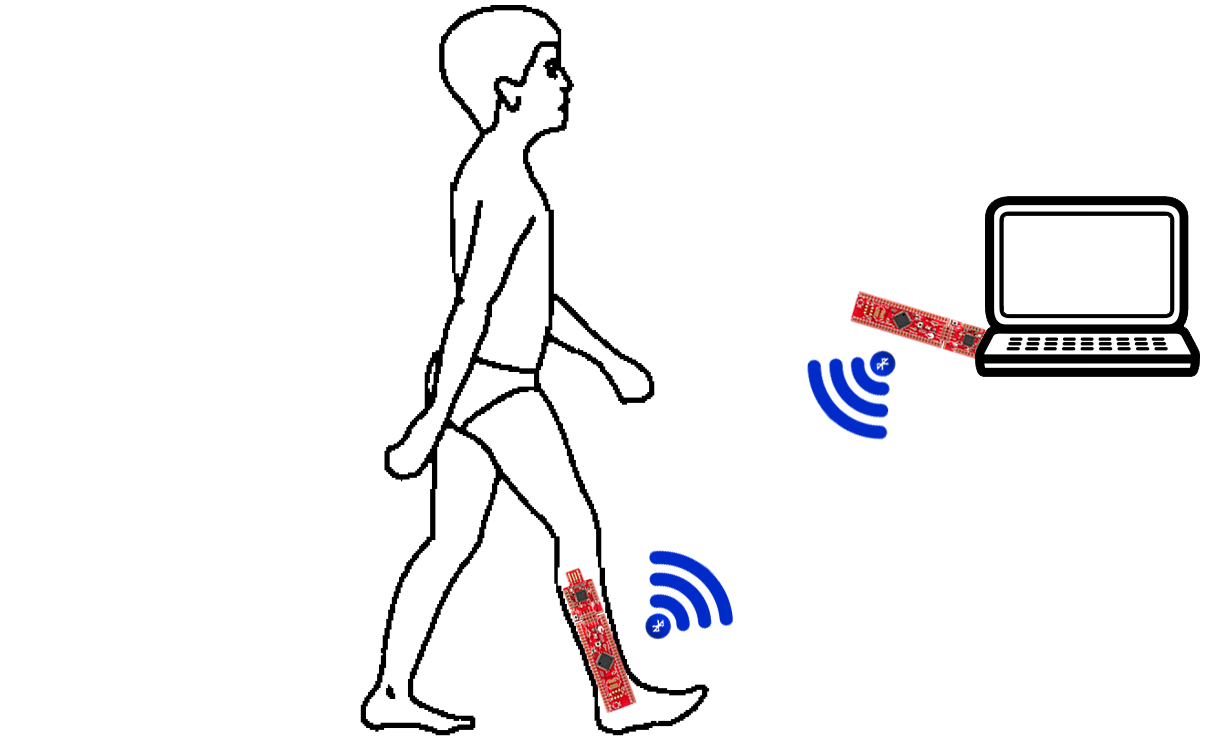
\includegraphics[width=.75\textwidth]{figures/forside2.PNG}
		\end{minipage}
		\hfill
	\end{figure}
	\vspace*{\fill}
	\scshape % Small caps
	{\Large Gruppe 4403\par}
	
	\vspace*{.8\baselineskip} % Whitespace between location/year and editors
	
	Aalborg Universitet,  01/02/2016 - 27/05/2016 \par % Location and year
\end{center} % Center all text
%{\color{white}X \\ X \\ X \\}

%\begin{center}
%	\textit{Gruppemedlemmer:}\\
%	Cecilie Sophie Rosenkrantz Topp, Frederik Skou Nielsen \\
%	Josefine Dam Gade, Line Sofie Hald, Morten Skaarup Larsen
%\end{center}
\begin{center}
	\line(1,0){400}
\end{center}
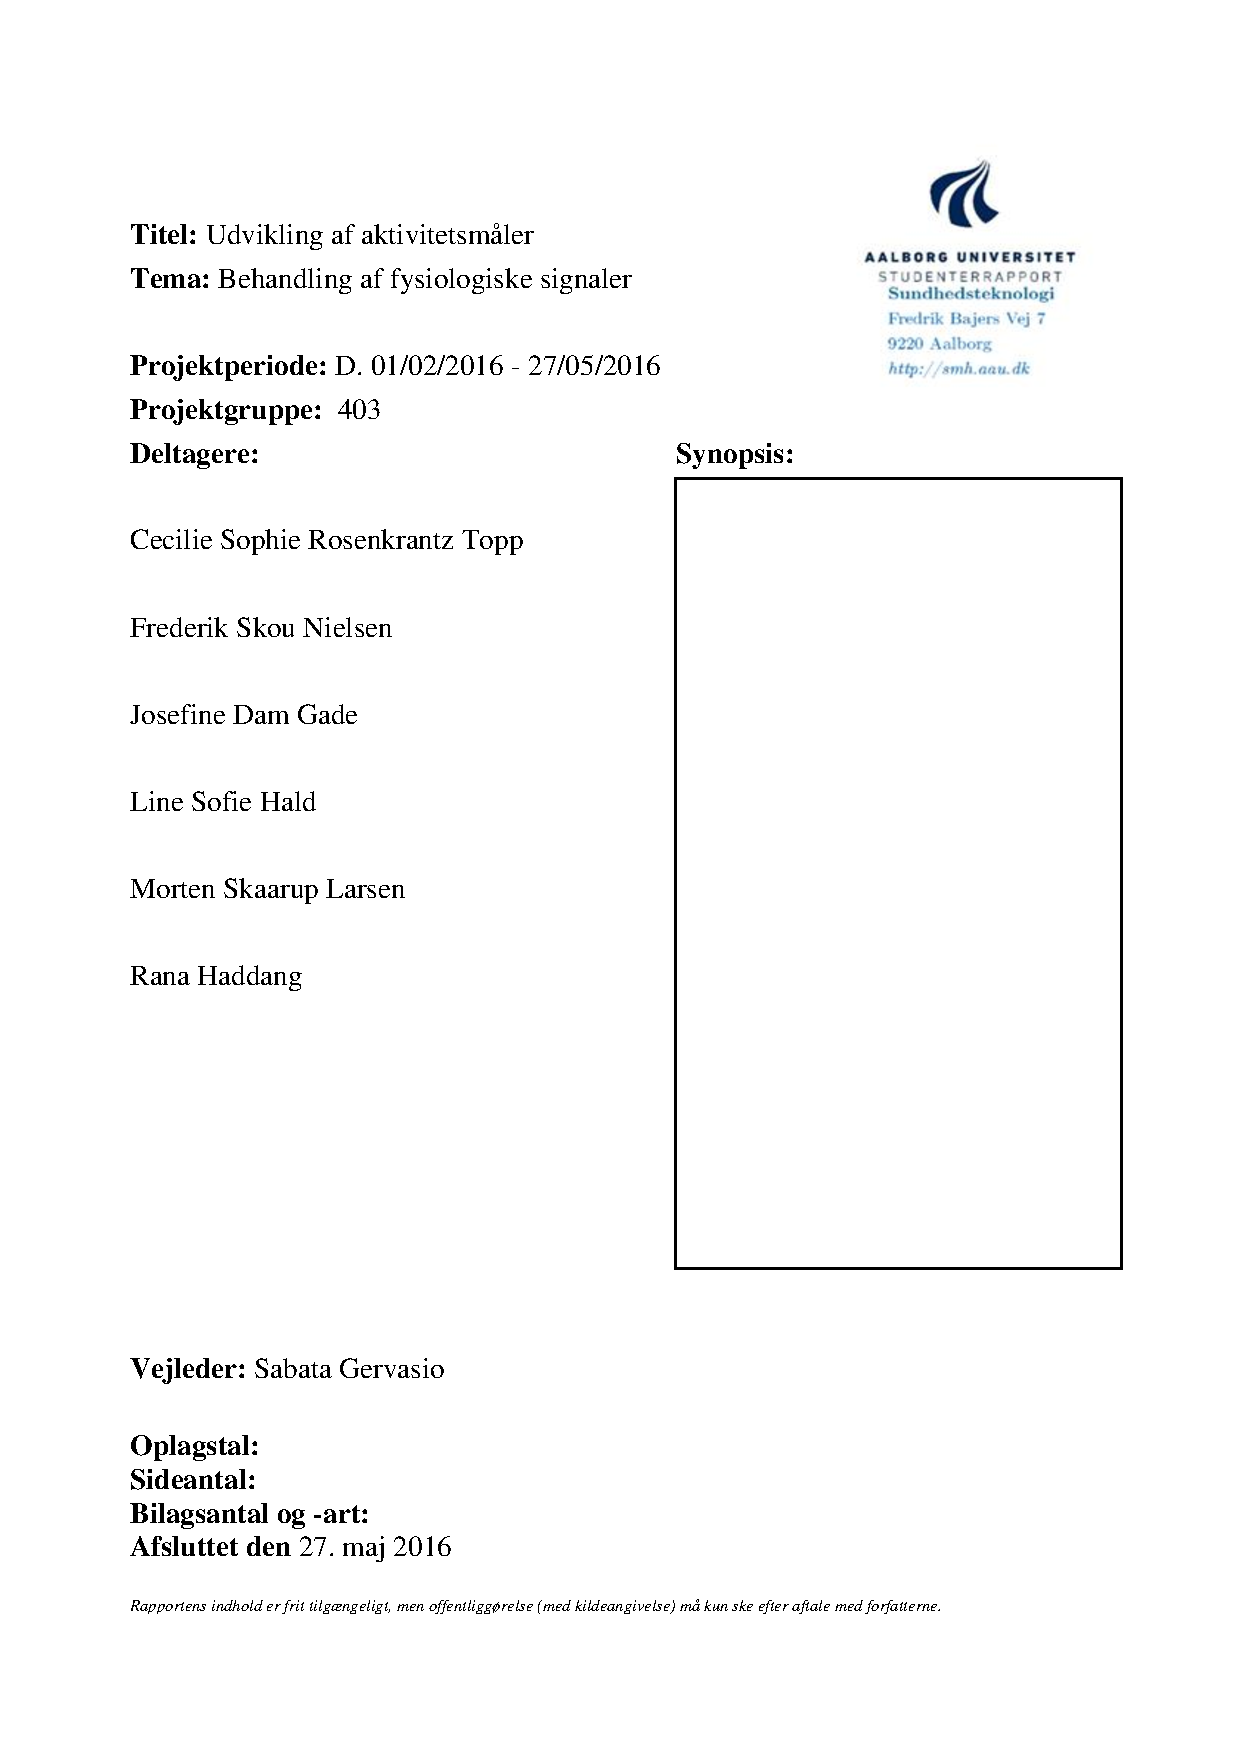
\includepdf[pages={1}]{rapportAfsnit/pFormaliteter/synopsis.pdf} \clearpage 
\chapter*{Forord og læsevejledning}
% !TeX spellcheck = da_DK
\section*{Forord}
Denne rapport er udarbejdet som et 4. semesters projekt på bacheloruddannelsen Sundhedsteknologi, Aalborg Universitet. Projektetperioden forløb fra februar 2016 til maj 2016. \\
Projektet tager udgangspunkt i studieordningen for bacheloruddannelsen i Sundhedsteknologi. Det fremgår, at semesterets fokusområde er 'Behandling af fysiologiske signaler'. Projektgruppen har derfor valgt at 
Dette projekt tager udgangspunkt i projektforslaget 'Udvikling af aktivitetsmåler', hvor formålet blandt andet er design, implementering og test af en prototype, der kan detektere fysisk aktivitet. Protoypen udvikles med henblik på at bestemme det fysisk aktivitetsniveau for børn i aldersgruppe 9-12 år. Prototypen vil derfor involvere en dataopsamling i form af analoge komponenter fra et accelerometer, et gyroskop og en pulssensor. Ydermere vil prototypen indeholde signal- og databehandling som muligøre digital visualisering på et grafisk brugerinterface.

%Projektet henvender sig til studerende på samme niveau eller andre interessere med et kendskab til basal analog og digital databehandling. \\
Der rettes en tak til vejleder Sabata Gervasio for et godt og lærerigt samarbejde under udarbejdelsen af denne rapport. Yderligere rettes der en tak til semesterkoordinater, John Hansen, for råd og vejledning til forståelse af semesterets nye mikrokontroller. 

\section*{Læsevejledning}
Projektet er opbygget af 5 kapitler, litteraturoversigt samt bilag. Før hvert kapitel er der et indledende kursiv afsnit, som har til formål at vejlede læseren i form af det følgende kapitels indhold og sammenhæng i rapportens helhed.\\
Første kapitel består af en indledning og initierende problemstilling. Herefter er problemanalysen, der bearbejder den initierende problemstilling og leder ud i en problemformulering. Det tredje kapitel er problemløsning, hvori blandt andet løsningsstrategi og essentielle teoretiske elementer hertil beskrives. Yderligere indeholder kapitlet krav til protoypen og dets delelementer. Det efterfølgende kapitel består af design, implementering og test af prototpyens delementer samt en test af den samlede prototype. Afslutningsvis er syntesen, indeholdende diskussion, konklusion og perspektivering.

Rapporten benytter Vancouver metoden til kildehenvisning, hvor den første kilde i litteraturoversigten er [1], den næste [2] og så fremdeles. Alle benyttede kilder er at finde i kapitel 5, hvor de er listet i numerisk rækkefølge. I tilfælde, hvor kilden befinder sig inden for punktum, tilhører denne kildehenvisning indholdet i den pågældende sætning sætning. Er kildehenvisningen placeret efter punktummet i sætningen, da tilhører kilden indholdet i det ovenstående afsnit indtil forrige kildehenvisning. \\
Tabeller og figurer er nummereret efter deres respektive afsnit, hvorfor eksempelvis figur 1.1 er den første figur i kapitel 1.

Rapporten benytter forkortelser, hvor ordets fulde længde skrives første gang ordet præsenteres, med tilhørende forkortelse i parantes efter ordet. Efterfølgende vil denne forkortelse benyttes i resten af rapporten, med undtagelse af overskrifter. 
\newpage

%the '*' allows the tableofcontents be excepted from the actual table of contents.
\tableofcontents*

%numbers the pages with Arabic numeral - starts from 1.
\mainmatter

% Indledning
\chapter{Introduktion}\vspace{-.75cm}
\textit{Dette kapitel belyser de samfundsmæssige problemstillinger, som forekommer i forbindelse med inaktive børn. De opstillede problemstillinger vil danne grundlag for et initierende problem, som yderligere undersøges i problemanalysen.}

\section{Indledning}
Fysisk inaktivitet er et stigende problem i det danske samfund, hvor 45~\% af danske børn i alderen 11-15 år er fysisk inaktive \citep{Sundhedsstyrelsen2006}. Desuden påpeger studier, at menneskers fysiske aktivitetsniveau er faldende med alderen. Som følge af et lavt fysisk aktivitetsniveau kan dette medføre en række helbredsmæssige konsekvenser \citep{Sundhedsstyrelsen2006}. Dette har resulteret i, at fysisk inaktivitet er relateret til 4.500 dødsfald årligt. Endvidere er det påvist, at fysisk inaktive personer ofte lever 5-6 år mindre end fysisk aktive personer. \citep{RISIKOFAKTORER} Det anses derfor som væsentligt at give børn fysisk aktive vaner i barndommen, for dermed at sikre et højt helbredsniveau \citep{L.MeyerP.Gullotta2012}. \newline
Fysisk inaktivitet kan være medvirkende til en række helbredsmæssige konsekvenser, heriblandt overvægt. Overvægtige børn har en stor risiko for at udvikle
livsstilssygdomme, såsom type-2-diabetes og hjertekarsygdomme. Ydermere har undersøgelser vist, at overvægtige børn har 70~\% risiko for at forblive overvægtige som voksne. \citep{Reilly2006}. Overvægt, og særligt fysisk inaktivitet, har desuden en stor betydning for barnets psykiske velvære. Danske børn har det seneste årti haft en faldende vurdering af deres livstilfredshed, som følge af deres fysiske fremtonen og formåen \citep{Universitet2014,StatensInstitutforFolkesundhed2007}. \newline
Fysisk inaktivitet har helbredsmæssige konsekvenser for den pågældende person, hvilket ydermere kan medføre konsekvenser for samfundet. Studier har påvist, at fysisk inaktivitet er relateret til et årligt medforbrug på 3,1 milliarder kroner for det danske sundhedsvæsen. \citep{RISIKOFAKTORER}

I sammenhæng med moderne teknologi og udviklingen af elektroniske spil samt sociale medier, foretrækker mange børn stillesiddende aktiviteter fremfor fysiske aktiviteter \citep{Universitet2014}. Dette har medført konsensus om, at teknologiens udvikling er en af hovedårsagerne til at fysisk inaktivitet er en stigende tendens, særligt hos børn \citep{Kiens2007}. \newline
Særligt børn i den tidlige pubertet har fået et øget tidsforbrug i forbindelse med stillesiddende aktiviteter. En undersøgelse har vist, at 15~\% af 11-årige børn i år 2000 brugte mere end 4 timer på elektroniske spil. I år 2014 var der sket en fordobling af dette tal, hvormed 30~\% af 11-årige brugte mere end 4 timer på elektroniske spil. \citep{SKOLEBØRNS} \newline
Der fremkommer en tydelig sammenhæng mellem fysisk inaktivitet og teknologiens udvikling. Dette kan være som følge af børns psykiske tilstand, idet særligt børn i den tidligere pubertetsalder finder spil og leg interessant \citep{Wied2011}. Spil og leg i forbindelse med teknologi er dermed motiverende elementer for børn som skal udføre en aktivitet. En sammenkobling af disse motiverende elementer og fysisk aktivitet har firmaet PlayWare implementeret på en række legepladser. PlayWare indeholder intelligent teknologi som motiverer børn til at få et øget fysisk aktivitetsniveau. Denne sammenkobling af teknologi, leg og fysisk aktivitet som PlayWare benytter, har resulteret i et øget fysisk aktivitetsniveau idet teknologien initierede en række fysiske aktiviteter hos børnene \citep{Rishoej2010,PDF}. 

\section{Initierende problemstilling}
Der er et stigende antal børn, som i dag er inaktive og overvægtige. Inaktive børn, der lever en stillesiddende livsstil, udsættes med forøget risiko for en lang række følgesygdomme. For at kunne motivere børn til en mere fysisk aktiv hverdag ønskes der en teknologisk tilgang til problemet:

\begin{center}
\textit{Hvilke teknologiske muligheder findes der for at motivere inaktive og overvægtige børn til et øget aktivitetsniveau?}
\end{center}

% Problemanalyse
\chapter{Problemanalyse}\vspace{-.75cm}
\textit{For at kunne løse den initierende problemstilling, analyseres en række aspekter af problemet. Dette gøres med henblik på at belyse problemet fra flere vinkler, hvorefter en problemformulering kan opstilles. \newline 
I dette kapitel beskrives fysiologisk inaktivitet og aktivitet samt dets indvirkning på kroppen. Derudover defineres en målgruppe for projektet, hvilket gør, at denne målgruppes motivationsfaktorer kan forklares. Dette giver nogle succeskriterier til aktivitetsmålere, der benyttes til at udvælge og analysere eksisterende aktivitetsmålere.}

\section{Effekt af fysisk aktivitet for børn}\label{sec:fysio}
\textit{I afsnittet beskrives, hvilke fysiologiske konsekvenser der er forbundet med inaktivitet og aktivitet. Det belyses hvilke forskelle der er på inaktivitet og overvægt, og hvilken der på længere sigt kan have de største fysiologiske konsekvenser. Derudover beskrives intensiteten af en fysisk aktivitet, og i hvilken grad den kognetive respons afhænger af fysisk aktivitet.}

%I forhistorien, da mennesket var jægere, var der en naturlig favorisering af de mennesker, som kunne lagre fedt bedre end andre, da der kunne gå lang tid imellem måltiderne, hvilket ikke er nødvendigt med den moderne livsstil, hvor teknologi og højere velstand har medført et mere fysisk inaktivt liv samtidig med der er let adgang til føde. Idet evolutionen ikke har tilpasset sig denne moderne livsstil, søger kroppen stadig at lagre fedt, hvorved personer med et lavere aktivitetsniveau end den energi de indtager, langsomt vil ophobe fedtdepoter, hvilket kan resultere i overvægt.\citep{Ahmad2014,Kiens2007}

\subsection{Fysiologisk risici ved inaktivitet}\label{subsec:inover}
%{\color{red} \textbf{Vi vil sørge for, at dette afsnit fokuserer lidt mere på at man kan både være aktiv men også overvægtig. Desuden vil vi gå lidt mere i dybden med de fysiologiske konsekvenser af at være inaktiv og overvægtig.}}
Hvis et individ udfører mindre end 2,5 times fysisk aktivitet om ugen med moderat intensitet, defineres vedkommende som værende fysisk inaktiv. Moderat intensitet defineres som aktivitet hvor personen skal opnå 64-74\% af maxpuls\fxnote{Moderat intensitet svarer til 40-59\% af den maksimale iltoptagelse, eller 40-59\% af pulsreserven (maxpuls – hvilepuls), eller 64-74\% af maxpuls eller 12-13 RPE (rate of percieved excertion, Borgskala) og er yderligere defineret som fysisk aktivitet, hvor man bliver lettere forpustet men hvor samtale er mulig}. \citep{Kiens2007} Overvægt og inaktivitet hænger ofte sammen, idet inaktivitet har en stor sammenhæng med overvægt. Grundlæggende opstår overvægt som resultat af et større kalorieindtag i forhold til ligevægtsindtag. \citep{Nestle2014} Definitionen for overvægt er blandt andet defineret igennem body mass index (BMI), hvilket er forholdet mellem en persons vægt og højde \citep{Academic2016}. Der findes en specifik BMI oversigt for henholdsvis piger og drenge i aldersgruppen 2-20 år, hvor grænseområder er fast defineret for begge køn. Der er ikke signifikant forskel på denne BMI oversigt imellem kønnene, men derimod afhænger grænseområderne for BMI oversigten af alderen. \citep{DiseaseControl2015}\newline
Fysisk inaktivitet og overvægt er ikke det samme, hvoraf de helbredsmæssige konsekvenser tilsvarende ikke er ens. Det er derfor muligt at være overvægtig men samtidig have en aktiv livstil. \citep{Kiens2007} Undersøgelser viser, at en overvægtig men aktiv person kan have samme metabolske sundhed som en normalvægtig. En overvægtig person kan igennem en aktiv livsstil nedsætte insulinresistens, højt kolesterol og højt bloktryk, selvom vedkommende forbliver overvægtig. \citep{Lunau2012,Marcelino2012}

%Det er veldokumenteret, at der sker et fald i fysisk aktivitet med alderen samtidig med, at der sker en stigning i vægt \citep{Kaprio2008}. Undersøgelser tyder på, at hvis kroppens cellulære vedligeholdelse styrkes med fysisk aktivitet kan aldringsprocessen nedsættes \citep{Knight2012}. 
%Fysisk inaktivitet forstærker altså den generelle aldring og anses som værende mindst lige så farligt som overvægt. De to fænomener forekommer dog ofte samtidig, da inaktivitet kan forsage overvægt, men fysisk inaktivitet har en selvstændig helbredsmæssig betydning ligesom overvægt. Det er muligt at være overvægtig men samtidig have en aktiv livsstil. \citep{Kiens2007,Kaprio2008,Hjort1997} 

Fysisk inaktivitet kan lede til flere af de store folkesygdomme som hjertekarsygdomme, diabetes, osteoporose og psykiske lidelser. Menneskekroppen er ikke skabt til at være inaktiv, og derfor vil kroppen reagere kraftigt på det. Eksempelvis kan kroppen begynde at nedbryde knoglerne indefra, således det fysiske aktivitetsniveau får betydningen for knoglernes samlede vægt, da der ikke er behov for store og stærke knogler, hvis de ikke benyttes tilstrækkeligt. \citep{Kiens2007,Reshma2002,Martini2012} \\
%Derudover kan inaktivitet lede til disuse syndromet, som blandt andet indebærer svækket hud integritet, ændret respiratorisk funktion og nedsætning af sanserne \citep{Knight2012,Mosby2009}.\\
Ifølge et longitudinelt studie fra Holland, hvor børn og unge blev fulgt over en 15-årig periode, har inaktivitet hos børn før puberteten alvorlige konsekvenser. Studiet konkluderede, at inaktivitet før puberteten medfører stor risiko for knoglefrakturer og mulig immobilitet herfra. Dette er et resultat af, at fysisk aktivitet i barndom og ungdom er stærkt relateret til knoglemineraltætheden i ryggen og hoften. \citep{Kemper2000} I et andet studie med 2.429 børn i alderen 5-14 år blev det konkluderet, at fysisk inaktive børn havde mere end dobbelt så stor risiko for høfeber end aktive børn \citep{Kohlhammer2006}. Inaktivitet i barndommen kan altså være særligt skadeligt, da det medfører kroniske konsekvenser.

Fysisk inaktivitet kan føre til overvægt, hvormed overvægt ligeledes kan medføre en række helbredsmæssige konsekvenser for den pågældende person. Overvægt øger risikoen for forhøjet kolesteroltal, forhøjet blodtryk og diabetes og følgesygdomme heraf som slagtilfælde og nyresygdomme. Det er dokumenteret, at der er større risiko for tidlig død, jo tidligere den pågældende person pådrager sig overvægt. Det er derfor essentielt at øge børns aktivitetsniveau og dermed mindske risikoen for inaktivitet i kombination med overvægt. \citep{Nestle2014} Derudover ses der, at overvægtige børn ofte lider af psykologiske og sociale problemer, hvilket kombineret med overvægten kan have en negativ indvirkning på barnets fremtid i forhold til uddannelse og socioøkonomiske status \citep{Academic2016}.

%Der er udarbejdet en specifik oversigt for børn i denne aldersgruppe, da et BMI på for eksempel 20 for en femårig ikke er det samme som for en tolvårig. En femårig med dette BMI vil være defineret som kraftig overvægtig, mens en tolvårig vil være inden for den normale zone. Der er ikke signifikant forskel imellem kønnene, men BMI for denne aldersgruppe afhænger meget af alderen. \citep{DiseaseControl2015}\\
%Overvægt opstår grundlæggende fordi der indtages mere energi end der forbruges. Nogle mennesker kan lagre fedt bedre end andre, hvorfor overvægt også kan være genetisk betinget. \citep{Nestle2014}\newline

%Definitionen for overvægt er globalt sat ud fra et body mass index (BMI), hvilket er forholdet mellem en persons vægt og højde\citep{Academic2016}. Der findes en BMI oversigt for henholdsvis piger og drenge i aldersgruppen 2-20 år, hvorefter grænseområderne for, hvornår en person er undervægtig, normal, overvægtig eller kraftig overvægtig er fast defineret for begge køn. Der er udarbejdet en specifik oversigt for børn i denne aldersgruppe, da et BMI på for eksempel 20 for en femårig ikke er det samme som for en tolvårig. En femårig med dette BMI vil være defineret som kraftig overvægtig, mens en tolvårig vil være inden for den normale zone. Der er ikke signifikant forskel imellem kønnene, men BMI for denne aldersgruppe afhænger meget af alderen. \citep{DiseaseControl2015}\\
%Overvægt opstår grundlæggende fordi der indtages mere energi end der forbruges. Nogle mennesker kan lagre fedt bedre end andre, hvorfor overvægt også kan være genetisk betinget. \citep{Nestle2014}\\
%Overvægt øger risikoen for højt kolesteroltal, forhøjet blodtryk og diabetes samt følgesygdomme heraf som slagtilfælde og nyresygdomme. Det er dokumenteret, at der er størst risiko for tidlig død jo yngre mennesker opnår overvægt. Det er derfor essentielt at forbedre børns aktivitet og dermed mindske risikoen for overvægt. \citep{Nestle2014} Derudover ses der, at overvægtige børn ofte lider af psykologiske og sociale problemer, hvilket kombineret med overvægten kan have en negativ indvirkning på barnets fremtid i forhold til uddannelse og socioøkonomiske status \citep{Academic2016}.

Det tyder på, at inaktivitet er mere skadeligt end overvægt, hvis de sammenlignes som inaktiv normalvægtig mod aktiv overvægtig.
Inaktivitet kombineret med overvægt øger risikoen for diverse sygdomme, men en normalvægtig inaktiv person er i større risiko for tidlig dødsfald end en overvægt aktiv person. I et 12-års studie lavet over 334.161 europæiske deltagere blev fysisk aktivitet, BMI og taljemål holdt op mod dødeligheden iblandt deltagerne. Igennem studiet konkluders det, at dobbelt så mange vil dø af inaktivitet i forhold til overvægt. Det antydes igennem dette, at inaktivitet er en større risikofaktor i sammenhæng med dødelighed. \citep{Ekelund2015} 
%En aktiv overvægtig person har derudover ikke større chance for at udvikle hjertesygdomme end normalvægtige, så længe de er trænede og dyrker motion \citep{Nichols2014}. 
\subsection{Fysiologisk udbytte ved aktivitet}\label{subsec:fysio_aktivitet}
Fysisk aktivitet er defineret som enhver bevægelse, hvor skeletmuskler skal kontrahere og derved forbrænde energi. Der er forskellige former for fysisk aktivitet, som har forskellige intensitetsniveauer. \citep{Academic2016a} Ifølge Sundhedsstyrelsen skal et barn i alderen 5-17~år være fysisk aktiv i mindst 60 minutter om dagen med moderat til høj intensitet. Derudover anbefales det, at børn i denne alder skal indgå i en aktivitet i 30 minutter med høj intensitet tre gange om ugen. Det vil dermed være fordelagtigt for barnets helbredsniveau at følge disse anbefalinger. \citep{Sundhedsstyrelsen2016}\newline
Fysisk aktivitet kan mindske risikoen for flere kroniske sygdomme såsom overvægt, diabetes og hjertekarsygdomme. Eksempelvis kan overvægt både forbygges og afhjælpes af fysisk aktivitet. Ydermere er fysisk aktivitet et forebyggende samt udviklende element for børns led, knogler og muskler. Eksempelvis dannes der mere synovialvæske ved fysisk aktiviteter, hvorved bevægelse af led faciliteres. Knogler vedligeholdes desuden af fysisk aktivitet, hvorved det kan undgås, at knoglens densitet mindskes som beskrevet i \secref{subsec:inover}. Ydermere udvikles og vedligeholdes muskler ligeledes af fysisk aktivitet, som følge af den belastning en fysisk aktivitet påfører muskelfibrene.  % Aktivitet medfører forbrænding af denne indtagede energi, hvorved ligevægtsindtaget muligvis ikke overskrides.
\citep{Academic2016a,Smith1991,Academic2016b,Cotman2007,CenterforDiseaseControlandPrevention2015}

Kroppens reaktion på fysisk aktivitet afhænger blandt andet af aktivitetens krav til kroppen\fxnote{Skal muskelgrupper fremskynde en position som ved svømning og derved være udholdende eller skal muskelgrupper løfte en vægt som ved vægtløftning og derfor være eksplosiv men knap så udholdende} og intensiteten heraf. %Ved anstrengende fysisk aktivitet overtager sympatikus størstedelen af det autonome nervesystem og sætter for eksempel fordøjelsen på pause, da fordøjelse ikke længere er førsteprioritet og al kroppens energi kan bruges til aktivering af de pågældende skeletmuskler. 
Eksempelvis tyder studier på, at fysisk aktivitet har en positiv indvirkning på børns kognition. \citep{SibleyEtnier2003} Ydermere vil en anstrengende fysisk aktivitet få hjertet til at slå hurtigt, hvilket medfører en øget puls, hvormed ilt og næringsstoffer hurtigere sendes rundt i kroppen \citep{Hjerteforeningen}. Blodkar vil desuden blive udspilet, således blodet i større grad kan komme til hudoverfladen og afgive den varme, som blodet fører væk fra de aktive muskler. Der sker altså en stigning i pulsen og blodtrykket, og denne stigning afhænger af den pågældende aktivitets påvirkning på kroppen. \citep{Martini2012,Stanfield2013,Berchtold2010}
\subsubsection{Aktivitet og intensitet}
Der findes en klar sammenhæng imellem puls og kroppens reaktion på motionen. Ifølge flere studier hænger procenten af den maksimale puls sammen med, antallet af forbrændte kalorier, om den aerobe udholdenhed trænes, forbedrer den anaerobe tolerance eller forbedrer den cardiovaskulære ydeevne\fxnote{hvilket gør, at man kan sprinte længere / er hurtigere, fordi der kommer mere ilt rundt i kroppen}. Jo højere procent intensitet, desto højere puls og hårdere fysisk træning. Denne sammenhæng inddeles i zoner som ses på \tabref{tab:PA_Procentpuls}. \citep{Leyland2007,Heartratejournal2015}
%\begin{figure}[H]
%	\centering
%	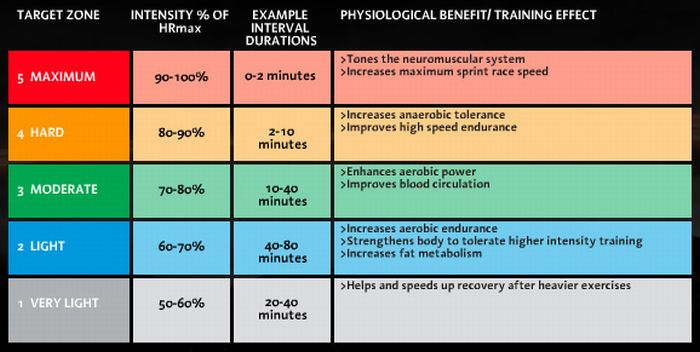
\includegraphics[scale=0.75]{figures/aProblemanalyse/heart-rate-zones.jpg}
%	\caption{På figuren ses fem zoner for kroppens reaktion i forhold til pulsraten. Der ses, at de fem zoner har hver sin påvirkning på kroppen. Det er dog også anbefalet, at varigheden i hver zone bliver lavere desto hårdere aktiviteten er. \citep{Heartratejournal2015}}
%	\label{fig:PA_Procentpuls}
%\end{figure}
\begin{table}[H]
	\centering
	\resizebox{\textwidth}{!}{%
	\begin{tabular}{@{}lll@{}}
		\rowcolor[HTML]{C0C0C0} 
		\multicolumn{1}{c}{\cellcolor[HTML]{C0C0C0}Zoner} & \multicolumn{1}{c}{\cellcolor[HTML]{C0C0C0}\begin{tabular}[c]{@{}c@{}}Intensitet \%\\ af maxpuls\end{tabular}} & \multicolumn{1}{c}{\cellcolor[HTML]{C0C0C0}Fysisk effekter}    \\
		\multicolumn{1}{l}{5 - Maksimum}                & \multicolumn{1}{l}{90-100 \%}           & \multicolumn{1}{l}{Træner det neuromuskulære system og øger maksimal sprinthastighed.}   \\ \hline
		\multicolumn{1}{l}{4 - Hård}                    & \multicolumn{1}{l}{80-90 \%}  & \multicolumn{1}{l}{Forbedrer den anaerobe tolerance og øger højhastigheds udholdenhed.}     \\ \hline
		\multicolumn{1}{l}{3 - Moderat}                 & \multicolumn{1}{l}{70-80 \%}  & \multicolumn{1}{l}{Øger aerob power og forbedrer blodcirkulationen.}      \\ \hline
		\multicolumn{1}{l}{2 - Let}                     & \multicolumn{1}{l}{60-70 \%}  & \multicolumn{1}{l}{\begin{tabular}[c]{@{}l@{}}Forbedrer den aerobe udholdenhed, styrker kroppen til høj intens\\ arbejde og øger fedtmetabolismen.\end{tabular}} \\ \hline
		\multicolumn{1}{l}{1 - Meget let}               & \multicolumn{1}{l}{50-60 \%}  & \multicolumn{1}{l}{Hjælper og øger hastigheden af genopbygningen af musklerne efter hårdt træning.}   \\ \hline
	\end{tabular}
	}
	\caption{I tabellen ses fem zoner for kroppens reaktion i forhold til pulsraten. Der ses, at de fem zoner har hver sin påvirkning på kroppen. Det er dog også anbefalet, at varigheden i hver zone bliver lavere desto hårdere aktiviteten er.\textit{(Revideret)} \citep{Heartratejournal2015}}
	\label{tab:PA_Procentpuls}
\end{table}

Det er dog omdiskuteret, hvorvidt zone 1 og 2 er de fortrukne, hvis ønsket er at tabe sig. Der forbrændes flere kalorier ved højintens aktivitet, altså i zone 4-5. I de lavintense zoner forbrændes kalorier fra fedtceller istedet for glykogen fra muskler, hvorfor kroppen efterfølgende vil lagre kalorier i fedtcellerne, som lider underskud. Hvis man derimod dyrker højintens arbejde, som svarer til zone 4 eller 5, vil glykogenen i musklerne forbrænde, og kalorier sendes derfor til musklerne, så de kan repareres og fortsætte arbejdet. De højintense zoner kan oftest ikke opretholdes over lang tid. \fxnote{Moderat intensitet svarer til 40-59\% af den maksimale iltoptagelse, eller 40-59\% af pulsreserven (maxpuls – hvilepuls), eller 64-74\% af maxpuls eller 12-13 RPE (rate of percieved excertion, Borgskala) og er yderligere defineret som fysisk aktivitet hvor man bliver lettere forpustet men hvor samtale er mulig. \citep{Kiens2007}} \citep{Martini2012,Leyland2007,Heartratejournal2015}. \newline
Pulsen er altså en faktor, som er medbestemmende for aktivitetens fokus. Dette medfører at pulsen er bestemmende for intensiteten, varigheden og udbyttet.
% !TeX spellcheck = da_DK
\subsubsection{Aktivitet og kognitiv respons}
Fysisk aktivitet har, som det er tilfældet med kroppens fysiske helbred, positive effekter for hjernens kognitive funktioner heriblandt indlæring, hukommelse samt koncentration. %kontrolprocesser, som multitasking, planlægning og koncentration. 
Derudover medvirker længerevarende træningsperioder til en positiv virkning på matematiske færdigheder\fxnote{Matematiske færdigheder} \citep{Bugge2015,Berchtold2010,Schmidt2015}.\\
Måden hvorpå fysisk aktivitet gavner hjernes kognitive funktioner er, at øget fysisk aktivitet resulterer i øget aktivitet i hippocampus, som er lokaliseret i det limbiske system i hjernen. Dette område i hjernen, processerer hukommelse og navigation, hvorved øget fysisk aktivitet forbedrer evnen til indlæring og hukommelse. Ved en længerevarende træningsperiode vil der ske en ændring i hjernens plasticitet, hvorved hjernen adapterer sig til det ændrede aktivitetsniveau\fxnote{Den tilpasser sig til at dyrke mere motion, hvorved området for indlæring og hukommelse vokser - ligesom en muskel man bruger mere}. Blodkarrene i hjernen\fxnote{hippocampus, cortex og cerebellum} udvides, som følge af det øgede aktivitetsniveau, på samme vis som i resten af kroppen\fxnote{reference til fysiologiafsnit}, hvilket medfører at der kan tilføres flere næringsstoffer og mere energi. \citep{Cotman2007}\\
Den fysiske aktivitets effekter på hjernens kognitive funktioner er dog ikke permanente, og aftager langsomt efter aktiviteten er opholdt. Efter fysisk aktivitet i 11-20 minutter, vil de øgede kognitive funktioner for børn vare i op til 50 minutter, mens de for voksne vil vare i 25-45 minutter. \citep{Cotman2007} Ydermere tyder studier på, at fysisk aktivitet kan have en længerevarende positiv effekt på børns kognition \citep{SibleyEtnier2003}.




\section {Udsat aldersgruppe for inaktivitet} \label{sec:maalgruppe}
\textit{Afsnittet præciserer en målgruppe for dette projektet i forhold til, hvilken aldersgruppe der er hensigtsmæssig at vælge, hvis inaktivitet skal mindskes i fremtiden. Derudover fokuseres der på hvordan børnene kan aktiveres.}
%\textit{Dette afsnit omhandler, hvilken aldersgruppe af inaktive børn, som vil kunne påvirkes til en mere aktiv livsstil som resultat af en teknologisk mulighed. Afsnittet beskriver, hvilken aldersgruppe af børn i grundskolen, der har den største tendens til at være inaktive, og hvilken aldersgruppe der vil tilknytte sig bedre aktivitetsvaner. Yderligere beskrives der, hvilken aldersgruppe, som vil finde leg og teknologi motiverende.}

Den teknologiske udvikling har stor betydning for den stigende andel af inaktive danskere %(den gamle sætning) Endvidere menes der, at den teknologiske udvikling kan have stor betydning for inaktivitet 
\citep{Kiens2007}. Ifølge Sundhedsstyrelsen var 45\% af danske 11–15 årige fysisk inaktive i 2006 \citep{Sundhedsstyrelsen2006}. Derudover mener de, at børn og unge bliver mindre aktive med alderen, hvilket kan have en sammenhæng med, at tilstedeværelsen af teknologi for børn stiger med alderen. %Denne målgruppe er under en udvikling, hvor tendensen tyder på, at desto ældre børnene bliver, jo mindre fysisk aktive er de. Halvdelen af børnene i denne aldersgruppe ønsker at leve en mere aktiv livsstil, med den rette mængde fysisk aktivitet. Med stor overvægt er det de inaktive børn, som har dette ønske, hvilket oftest ikke opnås. Det kan antages at de mangler den primære motivation for at opfylde denne lyst. Samtidig med, at en stor del af denne aldersgruppe er inaktive, så er antallet af 10-13 årige børn der cykler i skole, de seneste 15 år, faldet med 30\%. \citep{Sundhedsstyrelsen2006} 
I 2013 havde 3\% af børn i alderen 5-8 år teknologiske apparater med i skole hverdag, og i 2014 var dette steget til 33\% for samme aldersgruppe. Denne tendens, hvor teknologiske apparater medbringes dagligt, stiger med alderen, da 87\% af børn i aldersgruppen 9-12 år dagligt medbragt teknologiske apparater i 2014. \citep{Sundhedsstyrelsen2006,GjensidigeForsikring2014}

Børns vaner i forhold til deres fysiske aktivitetsniveau dannes i barndommen og den tidlige pubertetsalder \citep{F.SallisG.Simons-MortonJ.Stone1992}. For denne alder har autoritære roller, såsom forældre og lærere, fortsat en stærk påvirkning med henhold til at inkorporere vaner hos børnene \citep{L.MeyerP.Gullotta2012}. \newline
Det anses som nødvendigt, at børn vænnes til at være fysisk aktive i en tidlig alder, da vaner bringes med videre til voksenlivet. Hvis ikke børnene får en fysisk livsstil, vil vænnes de til en stillesiddende adfærd \citep{Nabe-NielsenSundhedsministerietetal.2005,P.J.KremersBrug2008,L.MeyerP.Gullotta2012}. Endvidere påpeger studier, at det er fordelagtigt at give børn gode vaner før puberteten. Dette skyldtes en række fysiske og psykiske faktorer, som børnene undergår i puberteten. Gode vaner med en fysisk aktiv livsstil skal dermed videreføres til børnene forinden folkeskolens udskoling. \citep{F.SallisG.Simons-MortonJ.Stone1992,L.MeyerP.Gullotta2012,P.J.KremersBrug2008}


Der ønskes at reducere antallet af inaktive, hvormed der med fordel kan appelleres til børn inden pubertetsaleden. Når børnene aktiveres i denne aldersgruppe, er chancen større for videreførelse af vaner. For at aktivere børnene kan det med fordel gøres gennem teknologi, da børnene i stigende grad benytter dette, hvilket er en af de store grunde til inaktivitet. Der ønskes dermed at optimere aktivitetsniveauet for børn i aldren 9-12 år, da det er denne aldersgruppe der især bruger teknologien i for høj en grad. 

%Det ønskes at reducere antallet af inaktive børn ved at appellere til en målgruppe, som er bekendte og fortrolige med teknologiske apparater. Ydermere skal der være mulighed for at påvirke målgruppens vaner i forhold til aktivitetsniveau. 
%I den forbindelse anses børn i den tidlige pubertet som en essentiel målgruppe for videreførelsen af en aktiv livsstil. Dette gøres på baggrund af at børn i denne alder stadig har mulighed for at tilegne sig nye vaner, samtidig med at de har et stort kendskab til teknologier. 


%Det antages, at hvis ikke skolerne engagerer børnene til fysisk aktivitet, vil helbredsniveauet blive dårligere end tidligere. Skolerne skal derved være forløber for at give børnene gode vaner hvad angår deres fysiske aktivitetsniveau. \citep{L.MeyerP.Gullotta2012} \newline
%% Eksempel på afrunding %% 
%Det ønskes at reducere mængden af inaktive børn i grundskolen, og for at inddrage den målgruppe hvor en teknologisk metode vil have størst påvirkning, så skal ovenstående problemstillinger sammenkobles. Børn i alderen fra 11-15 år, er overvejende inaktive, og ligeledes er denne aldersgruppe også problematisk da 30~\% færre, fra 10 år, cykler til skole. De er i en alder hvor vaner tages til efterretning og de er vant til at omgås teknologiske apparater. Dette betyder at en teknologisk mulighed for at motivere inaktive børn til et øget aktivitetsniveau vil have størst påvirkning på børn i alderen fra 10 år og op. Når børnene kommer ind i puberteten fjernes fokus dog oftest fra barnlig leg og andre interesser, hvormed kommende teenagere ikke skal inkluderes som en del af målgruppen. 

Dermed er målgruppen for dette projekt defineret som børn i aldersgruppen 9-12 år.
\section{Motivationsfaktor til øget fysisk aktivitet}\label{motivation_boern}
\textit{Dette afsnit beskriver, hvad der kan motivere den valgte målgruppe til øget fysisk aktivitetsniveau. Dette gøres med henblik på at have et grundlag til at designe et motiverende teknologisk apparat til målgruppen.}

Motivation er menneskets drivkraft i forhold til opførsel og udførslen af handlinger~\citep{V.Brown2007}. Fysisk aktivitet bliver udført på baggrund af den enkelte persons motivation til en aktivitet. Motivationen til en given aktivitet kan deles op i to overordnede typer: Intrinsisk og ekstrinsisk. Den intrinsiske motivation omhandler individets drivkraft til at udføre en opgave. Denne type motivation fokuserer på individets holdning til aktiviteten, og hvordan aktiviteten kan opfylde personlige behov. Den intrinsiske motivation er derfor karakteriseret af interessen og glæden ved en aktivitet. Den ekstrinsisk motivation omhandler en ekstern påvirkning af et individ. Denne type motivation kan eksempelvis være forældres forventninger til et barns skolekarakterer eller sportsaktiviteter. Barnet udfører aktiviteten på baggrund af en ekstern motivation, som kan risikere at blive udført med frygten for at fejle. Ekstrinsisk motivation fokuserer derfor på effekten af en aktivitet udført med en ekstern motivation.~\citep{J.Sebire2013} 

Motiverende faktorer kan være aldersmæssigt betinget, hvorfor børn og voksne motiveres forskelligt. Dette kommer blandt andet som følge af det psykologiske stadie, som børn befinder sig i. Børn handler instinktivt og impulsivt, hvormed de kan have svært ved at fastholde koncentrationen på en given aktivitet. Derfor er det essentielt, at børn har en motivationsfaktor, som giver glæde og lysten til at udføre en aktivitet.~\citep{V.Brown2007} For børn er det væsentligt, at en aktivitet opleves sjovt, anerkendende og har sociale dimensioner. Der kan imidlertid opstå problemer ved fysiske gruppeaktiviteter, da børnene eksempelvis kan være forhindret i at møde til de givne tidspunkter. Det kan dermed være fordelagtigt, hvis en fysisk gruppeaktivitet ikke udelukkende afhænger af et fysisk fremmøde.~\citep{Wied2011,Romani2013}

Børn i målgruppen motiveres særligt gennem leg, hvor det er essentielt, at alle deltagere oplever succes ved aktiviteten. Børn i denne alder motiveres endvidere intrinsisk gennem en positiv tilgang, hvor der særligt fokuseres på de ting, som lykkes. Dermed bidrager frivillig fysisk aktivitet med intrinsisk motivation til det bedste udbytte for børn~\citep{J.Sebire2013}. Konkurrencer vil ofte være en del af sociale fysiske aktiviteter, idet børnene sammenligner sig med andre. Disse konkurrencer kan medføre nederlag og dårlige oplevelser for det enkelte barn. Det er dog essentielt at bibeholde barnets gode oplevelse ved den fysisk aktivitet. Konkurrencer skal derfor holdes på et plan, hvor det ikke er en begrænsende faktor for barnet. Overordnet skal der appelleres til børnene i denne aldersgruppe gennem fairplay og et positivt syn på aktiviteterne.~\citep{Wied2011}\\
Sociale sammenhænge, forældrenes støtte og leg igennem fysiske aktiviteter er de væsentligste ekstrinsiske motivationsfaktorer for børn, som skal øge det fysiske aktivitetsniveau. Generelt virker intrinsisk motivation bedre end ekstrinsisk motivation. Hvis barnet ikke selv har lysten og interessen i en given fysisk aktivitet, vil eksempelvis forældres opfordring ikke gøre en væsentlig forskel.~\citep{J.Sebire2013,McWhorter2003} En fysisk aktivitet, som giver børn naturlig tilfredsstillelse og glæde, kan medføre et fremtidigt øget fysisk aktivitetsniveau for barnet~\citep{Romani2013}.
\section{Aktivitetsmålere til børn} \label{tracker_intro}
%%Den gamle intro
%\textit{Dette afsnit omhandler, en beskrivelse af funktionaliteten for en række udvalgte aktivitetsmålere. Disse aktivitetsmålere bliver vurderet og analyseret på baggrund af opstillede succeskrav. Afslutningsvis præsenteres den samlede vurdering af aktivitetsmålerne, og hvordan disse opfylder opstillede kriterier.}
\textit{Dette afsnit omhandler de vurderede optimale egenskaber for en aktivitetsmåler samt funktionaliteten af nuværende aktivitetsmålere til børn. Hertil vil en række udvalgte aktivitetsmålere blive vurderet og analyseret på baggrund af opstillede succeskriterier. Afslutningsvis præsenteres den samlede vurdering af aktivitetsmålerne, og i hvilken grad disse opfylder de opstillede kriterier.}
%%Gammel indledning 
%
%Sundhedsstyrelsen anbefaler børn at motionere 2,5 ugentligt, hvis dette ikke opfyldes karakteriseres barnet som inaktivt. Manglende motion kan være som resultatet af den teknologiske udvikling, som medfører en mere stillesiddende livsstil. \citep{ObesityActionCoalition} Den teknologiske udvikling som medvirker til inaktivitet og stillesiddende livsstil, er forsøgt udnyttet som modarbejdende faktor. Flere producenter har benyttet teknologi som et led i at motivere børn til et mere aktivt liv \citep{Fuhu2015,PowerAbout2015}. Fælles for disse producenter er, at de motiverer børn til at fysisk aktivitet gennem spil og leg. Producenterne benytter aktivitetsmålere til at registrere aktivitet. Sideløbende belønnes børnene med et antal point, afhængigt af aktivitetsniveauet. Børnene har i mange tilfælde mulighed for at spille alene, men også i hold. Dette medfører en mulig implementering af motions motiverende teknologier i et skoleregi. \newline
%Potentialet af en teknologi som motiverer børn til en aktiv livsstil kan have flere fordele. Den primære fordel ved en aktiv livsstil er forebyggelsen af følgesygdomme. Dette har vist sig at være en fordelagtig økonomisk og sundhedsmæssig investering.
%% Ny indledning

\subsection{Aktivitetsmålere}
Aktivitetsmålere kan benyttes af alle aldersgrupper til at registrere det fysiske aktivitetsniveau. Den kan registrere data for en bestemt dag eller over en længere periode. Aktivitetsmålere benytter en eller flere sensorer til at registrere det fysiske aktivitetsniveau. Eksempelvis kan et pedometer, accelerometer eller gyroskop findes i en aktivitetsmåler. Et pedometer er bestemmende for…. \textbf{skriv teori ud fra det i problemløsning. Det handler blot om en sætning til hver sensor} \newline
Et fælles formål for aktivitetsmålerne er dermed at bestemme det fysiske aktivitetsniveau gennem en række analoge og digitale elementer. De digitale elementer benyttes til at bestemme og visualisere sensorens opsamlede data. Dermed er de digitale elementer blandt andet bestemmende for den brugerflade, som er tilhørende den pågældende aktivitetsmåler. En aktivitetsmåler, som er specifikt designet til børn, har muligvis en brugerflade, som involverer spil og leg for at motivere barnet til øget fysisk aktivitet. 

\subsection{Succeskriterier for aktivitetsmålere} \label{succeskrav}
Flere producenter har benyttet teknologi, som et led i at motivere børn til et mere aktivt liv gennem spil og leg ved hjælp af aktivitetsmålere. Børnene har i mange tilfælde mulighed for at spille alene eller sammen med andre. %, hvorfor det er muligt at implementere aktivitetsmotiverende teknologier i et skoleregi. 
\citep{Fuhu2015,PowerAbout2015} %Denne sammenkobling af teknologi og fysisk aktivitet er blandt andet udnyttet af firmaet Playware, som har haft positive resultater hvad angår motivering til øget fysisk aktivitetsniveau \citep{Rishoej2010}. \newline% Yderligere giver frivillig fysisk aktivitet med intrinsisk motivation det bedste udbytte for børn \citep{J.Sebire2013}. \newline
En teknologi, som motiverer børn til en aktiv livsstil, har potentielt flere samfundsøkonomiske og sundhedsmæssige fordele, idet en aktiv livsstil blandt andet er forebyggende for diverse følgesygdomme, som beskrevet i \secref{subsec:inover}.

Aktivitetsmålere til børn bør tage højde for en række essentielle kriterier, som blandt andet indebærer, at alt barnets daglig aktivitet registreres. Dermed skal systemet registrere og gemme al aktivitet igennem et barn hverdag, hvilket indebærer både skoleaktiviteter såvel som fritidsaktiviteter. I og med al fysisk aktivitet registreres vil der dannes en mere realistisk gengivelse af barnets aktivitetsniveau. \\%skal barnets samlede fysisk aktivitet i løbet af en dag, indeholdene fritidsaktiviteter såvel som skolerelaterede aktiviteter, kunne registreres og gemmes af systemet.  %Nævnt i \secref{subsec:fysio_aktivitet} anbefales det, at børn dagligt udfører 60 minutters aktivitet med moderart til høj intensitet. 
Et studie har undersøgt, hvilke børneidrætter der er de 10 mest populære blandt børn i aldersgruppen 7-15 år. Det fremgår af dette studie, at 7 ud af de 10 mest populære børneidrætter involverer gang eller løb \citep{Asserhoej2013}. Desuden fremgår det af flere  studier, at cykling er en af de hyppigst benyttede transportmidler for børn i alderen 10-15 år \citep{DTU2014,COWI2015}. På baggrund af dette skal en aktivitetsmåler kunne registrere gang, løb og cykling for dermed at kunne bestemme barnets samlede fysiske aktivitetsniveau i løbet af en dag. Ydermere skal aktivitetsmåleren kunne skelne mellem disse aktivitetsformer. Denne automatiske genkendelse kan udformes ved brug af flere forskellige sensorer. Herved kan aktivitetsmåleren opnå en stor brugervenlighed, idet barnet ikke selv skal indtaste, hvilken type aktivitet der vil blive udført. \newline
Intensiteten af en given fysisk aktivitet kan bestemmes af en persons puls, som det fremgår i afsnit \secref{subsec:fysio_aktivitet}. Det vil derfor være fordelagtigt, hvis aktivitetsmåleren kan bestemme barnets puls og herigennem kategorisere intensiteten samt den fysiske effekt af aktiviteten.
%
%Idet aktivitetsmåleren skal anvendes igennem en skoledag, så skal aktivitetsmåleren også kunne registrere aktivitetsformer, der er tilgængelige i skolen. Sundhedsstyrelsen har opstillet en række aktivitetsformer, hvor det ønskede intensitetsniveau opnås. Aktivitetsformer, som er tilgængelige for børn igennem en skoledag, er eksempelvis lege, der indebærer løb, leg i skolegården, cykling, fodbold og basketbold. Fælles for disse aktivitetsformer er, at de kan registreres som gang, løb og cykling. \citep{Sundhedsstyrelsen2003}
%I takt med at den daglige aktivitet opfanges bør en aktivitetsmåler kunne registrere, og dermed også adskille, gang, løb og cykling, hvilket gøres gennem forskellige sensorer.
%
%For at en aktivitetsmåler kan registrere aktivitet, kræves det at aktivitetsmåleren indeholder sensorer. Med den rette algoritme kan sensorer automatisk skelne mellem de nævnte former for aktivitet. 
%Idet de fysiologiske effekter i forbindelse med aktivitet er forskellige alt efter intensitetsniveauet, skal aktivitetsmåleren ydermere kunne registrere intensiteten af aktiviteten og belønne brugeren gennem brugerfladen.  

Målgruppen for den tilsigtede aktivitetsmåler er børn i aldersgruppen 9-12 år. Det er påvist, at børn i denne aldersgruppe motiveres bedst gennem frivillig fysisk aktivitet med intrinsisk motivation som leg og spil. Aktivitetsmåleren skal derfor kunne benytte sig af en type motivation, som henvender sig til målgruppens behov.

Aktivitetsmålerens placering og påmontering skal desuden være komfortabel. Aktivitetsmåleren må ikke fratage eller hindre barnets psykiske eller fysiske udfoldelse i forbindelse med afbenyttelse. 
%Da aktivitetsmåleren skal benyttes hovedsageligt af inaktive børn, skal den kunne motivere til fysisk aktivitet. Ifølge \secref{motivation_boern} tyder det på, at børn i den udvalgte målgruppe motiveres til aktivitet gennem leg og spil. Et essentielt kriterie vil derfor være at kunne motivere denne målgruppe uanset alder og køn. \newline
%En aktivitetsmåler skal ikke være til gene, da en eventuelt gene i forbindelse med placeringen muligvis vil medføre fravalg af benyttelse og derved fysisk aktivitet. Derfor er et yderligere kriterie, at aktivitetsmåleren ikke skal være til gene. Børnene med en aktivitetsmåler påsat skal være lige så frie som foruden.

Den optimale aktivitetsmåler skal dermed kunne: 
\begin{itemize}
\item Registrere gang.
\item Registrere løb.
\item Registrere cykling. %Når de står registreret hver for sig, så menes der derved, at de kan skelnes fra hinanden.
\item Registrere aktivitetens intensitet. %igennem puls
\item Motivere både fysisk inaktive og fysisk aktive børn. %socialt
\item Monteres og placeres på komfortabel vis.
\end{itemize}

\subsubsection{Afgrænsning af aktivitetsmålere}  %Hed før Baggrund for analyse og vurdering af aktivitetsmålere
Der er udvalgt fire aktivitetsmålere til videre analyse, som alle har samme formål; at motivere børn til et øget fysisk aktivitetsniveau. De udvalgte aktivitetsmålere henvender sig alle til børn i målgruppen 9-12 år og har derfor på forskellig vis udformet en brugerflade, som er motiverende for målgruppen. Ydermere er aktivitetsmålerne trådløse og tilbyder en brugerflade gennem trådløs overførsel i form af en hjemmeside og/eller app. \newline
De udvalgte aktivitetsmålere vil blive analyseret og vurderet på baggrund af ovenstående succeskriterier.

\subsection{UNICEF kid power band}
UNICEF Kid Power Band er en aktivitetsmåler, som appellerer til børn ved at hjælpe andre børn i ressourcefattige lande, hvoraf sloganet til aktivitetsmåleren udspringer: "Vær aktiv. Red liv". \newline
Aktivitetsmåleren, der er udformet som et armbånd, fremgår af~\figref{fig:unicef}. Aktivitetsmåleren benytter et pedometer og et accelerometer til at registrere barnets fysiske aktiviteter. \citep{PowerAbout2015,PowerManual2015}

\begin{figure}[H]
	\centering
	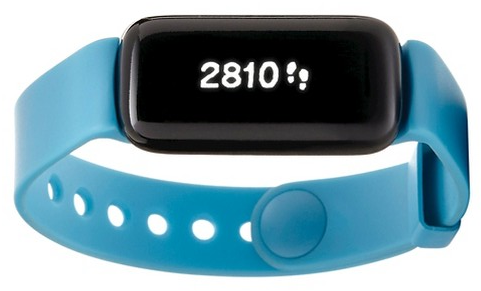
\includegraphics[scale=0.6]{figures/aProblemanalyse/unicef.png}
	\caption{På figuren ses UNICEF kid power band. \cite{Unicef2016}}
	\label{fig:unicef}
\end{figure}
Børnene kan optjene point ved at være fysisk aktive - desto mere fysisk aktive de er, desto flere point samler de sammen. Pointene omregnes til en sum penge, som sponsoreres af fans, firmaer og forældre. Pengene, som børnene dermed gør sig fortjent til gennem fysisk aktivitet, vil blive sendt til de ressourcefattige lande, som aktivitetsmåleren støtter. \newline
Børnene har mulighed for at vælge mellem en række udvalgte lande gennem såkaldte missioner. Disse missioner handler om at lære børnene om samfundet i det pågældende land, og giver dermed børnene indsigt i, hvor betydningsfuld deres hjælp er. Børnene har gennemført en mission, når de har været nok fysisk aktive til at have optjent alle point for den pågældende mission. \newline
Alle resultater samles i en app, hvor børnene både har mulighed for at følge med i progressionen for dem selv og deres venner samt for de missioner, som de deltager i. \citep{PowerAbout2015, PowerManuel2015} Aktivitetsmåleren har desuden en indkøbspris på 260 kr \citep{PowerAbout2015}. 
%
%For at optjene point, skal børnene gennemføre forskellige missioner, som professionelle atleter står i spidsen for, hvorigennem børnene ikke blot er aktive men også lærer om forskellige kulturer.\fxnote{Et eksempel er en mission, som basketballspilleren Tyson Chandler står i spidsen for, hvor børnene lærer om hvordan børn i ressourcefattige lande, hjælper familien med at gro deres eget mad.} \citep{PowerMission2015} 
%Børnene kan selv følge med i, hvor langt de er i den pågældende mission på aktivitetsmåleren eller gennem en applikation (app). Når børnene har gennemført en mission, omregnes deres point til en sum penge, sponsoreret af fans, firmaer og forældre, som sendes til det pågældende ressourcefattige land, som missionen støtter. \newline
%Hver dag nulstilles aktivitetsmåleren, så børnene hver dag kan følge med i hvor aktive de har været den pågældende dag. Derudover gemmes der data 30 dage tilbage, så det er muligt at sammenligne med tidligere dage. 
%På aktivitetsmåleren er der en skærm, hvor det er muligt at følge med i klokken, antal skridt, KidPower points, fremskridt på missioner og navnet på brugeren. 
%Alle resultater samles i en applikation (app), hvor børnene både har mulighed for at følge med i progressionen for dem selv og deres venner, samt for de missioner de deltager i. \citep{PowerAbout2015}

\subsubsection{Vurdering af succeskriterier} %%%%%%%%%%%%%%%%%%%%%%KOMMET HERTIL MED KOMMA%%%%%%%%%%%%%%%%%%%%%%%%%%%%%%%
Aktivitetsmåleren giver mulighed for at tælle skridt, som både registreres under løb, gang og andre aktiviteter, dog skelnes der ikke mellem aktiviteterne. Da armene ikke bevæges ved cykling, er dette ikke muligt for aktivitetsmåleren at registrere. Derudover måles intensitet af det udførte arbejde ikke, idet der udelukkende måles hvor energisk armene bevæges under en givne øvelse, og ikke puls, iltoptagelse eller anstrengelse. Aktivitetsmåleren er designet som et armbånd, som nemt kan sættes på barnet, da den har en justerbar rem. \citep{PowerManual2015} \newline
Børnene udfører de fysiske aktiviteter sammen med andre børn, med henblik på at hjælpe børn i ressourcefattige lande. Aktivitetsmåleren motiverer børnene på intrinsisk vis, grundet de sociale aspekter som ligger til grund for aktivitetsmålerens brugerflade.
%Børnene aktiveres socialt, da alle aktiviteter udføres med henblik på at de sammen med jævnaldrende, skal hjælpe børn i ressourcefattige lande. Derudover bliver børnene gennem appen opdateret på progression i de missioner de deltager i, samt venners progression, hvorved det ikke kun er den individuelle præstation der er i fokus. %Flere skoler i USA har i fjerde klasse også benyttet aktivitetsmåleren, som en del af klasseprojekter, for at få børnene til at blive mere aktive. 
\citep{PowerAbout2015} 

UNICEF Kid Power Band opfylder to ud af seks succeskriterier, mens det delvist opfylder to succeskriterier.

\subsection{The Sqord Booster}
The Sqord Booster er en aktivitetsmåler, som appellerer til børn i alderen 8-14 år gennem konkurrence og fællesskab. Måden hvorpå aktivitetsmåler motiverer børnene er gennem spil, hvori al aktivitet de udfører gemmes i en avatar. Denne avatar designer børnene selv på en hjemmeside, hvor de også kan kommunikere med deres venner. Forældrene har mulighed for at oprette et forældrelogin til siden, så de ligeledes kan følge med i deres børns aktivitet. Aktivitetsmåleren er designet til at blive brugt i grupper, dette er dog uafhængigt af om børnene fysisk eller online er sammen. \citep{Sqord_family2015} \newline
Børnene optjener point ved at deltage i forskellige konkurrencer, hvor deres aktivitet måles gennem et tre-akse accelerometer, som måler hastigheden af aktiviteterne. Aktivitetsmåleren placeres oftest om håndleddet som et armbånd, der kan ses på \figref{fig:sqord}, men kan også placeres i en lomme eller bundet til skoen, angiveligt uden indflydelse på målingerne som sensorerne udfører. \citep{Sqord_family2015} \newline Børnene kan enten konkurrere mod hinanden, eller arbejde sammen som et hold. Det er dog også muligt at benytte aktivitetsmåleren individuelt. Der er dermed ikke inkorporeret nogen konkurrencer i brugerfladen, men det er dog muligt at se andre børns progressioner, hvormed der indirekte kan opstå et konkurrende elemenet i forbindelse med aktivitetsmåleren\citep{Sqord_family2015,Sqord_group2015}
\begin{figure}[H]
	\centering
	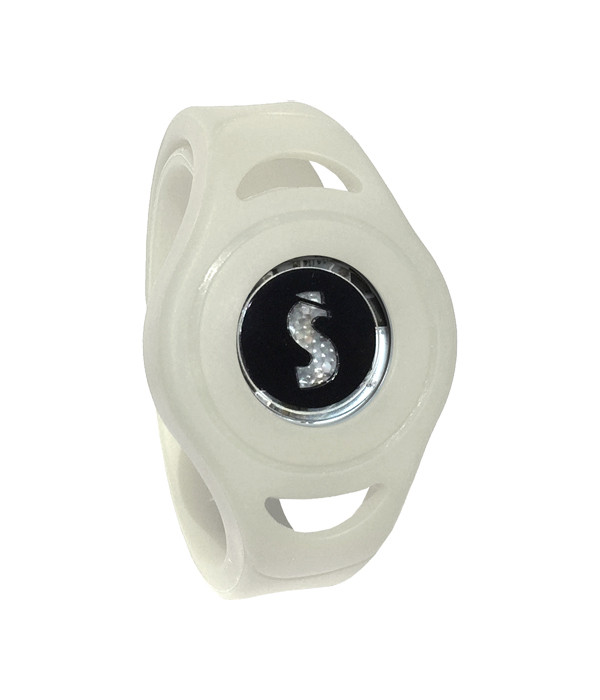
\includegraphics[scale=0.35]{figures/aProblemanalyse/sqord.JPG}
	\caption{På figuren ses The Sqord Booster sat i et armbånd. \citep{Sqord2016}}
	\label{fig:sqord}
\end{figure}
%Hjemmesiden hvor børnene kan følge med i deres avatar, fungerer som et forum, hvor de har mulighed for at give hinanden highfives for gode præstationer, chatte indbyrdes, eller lave talebobler, hvor alle kan se hvad de skriver. \citep{Sqord_family2015} \newline
The Sqord Booster tilgodeser alle præstationer, da alle får en medalje ved blot at have deltaget i en given aktivitet. Vinderen får imidlertid flere point end de andre deltagere. Spillet er lavet, så alle har mulighed for at vinde, da der i det enkelte spil, vurderes ud fra børnenes individuelle form, ved at se på tidligere præstationer. \citep{Sqord_family2015} \newline
The Sqord Booster har endvidere en indkøbspris på 230 kr \citep{Sqord_family2015}. 

\subsubsection{Vurdering af succeskriterier}
Aktivitetsmåleren registrerer både børnenes aktivitet ved gang og løb men kan ikke skelne mellem de to forskellige former for aktivitet, og der registreres ikke cykling. Der måles derudover ikke intensitet af det udførte arbejde, idet kun accelerometerets fart vurderes. \newline
Børnene bliver aktiveret socialt, da hjemmesiden er en blanding mellem et chatforum og en oversigt over præstationer. Derudover har børnene mulighed for at konkurrere med og mod hinanden. The Sqord Booster har derudover sørget for at fange både de børn der er i god form, og dem som ikke er, da alle har mulighed for at vinde baseret på tidligere præstationer. Aktivitetsmåleren er mulig at placere flere steder, hvormed børnene har mulighed for at vælge en placering, hvor det er til mindst gene.\fxnote{Derudover er det designet efter målgruppen, hvormed aktivitetsmåleren både kan modstå stød og tåle at komme i vand.}

The Sqord Booster opfylder to ud af seks succeskriterier, mens det delvist opfylder to succeskriterier.

\subsection{Nabi Compete}
Nabi Compete er en aktivitetsmåler, som appellerer til børn over seks år gennem deres madvaner og samvær med andre. Der er muligt for børnene at konkurrerer individuelt, men hovedformålet er at konkurrere mod eller med andre som et hold. Konkurrencerne kan bestå i at løbe en bestemt rute, som børnene selv kan designe og kan tegne ind. Desuden kan børnene vælge en fødevare i brugerfladen, og dermed vil brugerfladen fortælle barnet hvor meget det skal være fysisk aktiv for at have forbrændt kalorierne svarende til fødevaren. Der kan derfor være et konkurrende element i, at skulle forbrænde flest kalorier eller løbe længst.
%Det er muligt at opnå mål sammen med andre, eller dyste i hvem der når forskellige mål først. 
\fxnote{Derudover lærer børnene om kalorier og distance ved at bruge appen, hvor det er muligt at følge med i progressionen.}
Gennem konkurrencerne optjenes der point, som kan bruges til at købe et virtuelt dyr, som ved hjælp af point kan vokse. 
Aktiviteten måles gennem et tre-akse accelerometer, som sidder i et armbånd, hvilket kan ses på \figref{fig:nabi}. Dataet synkroniseres til en app gennem bluetooth, hvor der kan gemmes data i op til 90 dage, så barnet og forældrene dermed har mulighed for at følge med i barnets progression. \citep{Fuhu_tech2015,Fuhu2015} 
Nabi Compete har endvidere en indkøbspris på 190 kr \citep{Fuhu_tech2015}. 

\begin{figure}[H]
	\centering
	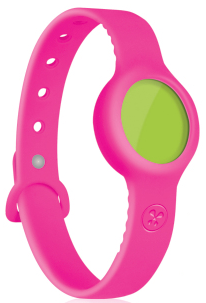
\includegraphics[scale=0.9]{figures/aProblemanalyse/nabi.png}
	\caption{På figuren ses Nabi Compete. \citep{Perez2015}}
	\label{fig:nabi}
\end{figure}

\subsubsection{Vurdering af succeskriterier}
Aktivitetsmåleren registrer både gang og løb, men det er ikke muligt at skelne mellem de to former for aktivitet, der registreres heriblandt ikke cykling eller intensitet med aktivitetsmåleren. 
Børnene aktiveres socialt, da appen er designet med mulighed for at konkurrere mod hinanden eller arbejde sammen i hold. Derudover har børnene mulighed for, 
%at have et kæledyr på appen, hvorved de, 
udover at konkurrere mod andre, kan se hvor mange kalorier de har forbrændt. Aktivitetsmåleren monteres uden gene, da den er placeret i en justerbar rem, som let kan monteres om barnets håndled.\fxnote{Derudover er den designet således at den kan tåle sved og regn, hvilket gør at børnene kan bruge det i al slags vejr.}

Nabi Compete opfylder to ud af seks succeskriterier, mens det delvist opfylder to succeskriterier.

\subsection{Ibitz}
Ibitz er en aktivitetsmåler, som apellerer til børn over fem år gennem udfordringer i samarbejde med forældrene. Ibitz har generelle udfordringer, men der lægges særligt op til at forældrene sætter nogle mål for børnene gennem deres dag og derved bestemmer udfordringerne. Forældrene har dermed mulighed for at lave en række opgaver til deres børn, som de vurderer er passende i forhold til barnets aktivitetsniveau. Barnet kan derfor vælge mellem disse tilpassede opgaver. \newline
Disse udfordringer kan indebære hvor meget tid børnene skal bruge på aktivitet og hvor land tid de må bruge på elektroniske spil. Ved at gennemføre udfordringerne forældrene eller Ibitz har sat, kan børnene tjene point, som kan bruges på to forskellige spil. \newline
%Dette kan være for hvornår der er legetid, hvornår de må sidde foran skærmen eller hvornår de skal lave aktiviteter med forældrene. 
Aktivitetsmåleren består af et pedometer, som måler skridt, der trådløst synkroniseres med en app via bluetooth. Aktivitetsmåleren monteres ved en klemme, som det fremgår af~\figref{fig:ibitz}. Appen gemmer aktiviteterne i 30 dage, hvorved barnet og forældrene har mulighed for at følge med i progressionen. 
Ibitz har endvidere en indkøbspris på 165 kr. \citep{Ibitz_features2016}

\begin{figure}[H]
	\centering
	
\includegraphics[scale=0.9]{figures/aProblemanalyse/ibitz.png}
	\caption{På figuren ses Ibitz klemmen.\citep{Ibitz_features2016}}
	\label{fig:ibitz}
\end{figure}

\subsubsection{Vurdering af succeskriterier}
Aktivitetsmåleren registrer både gang og løb, dog er det ikke muligt at skelne mellem de to former for aktivitet, samt at registrere puls og cykling. Børnene bliver delvist aktiveret socialt, hvor det primært er sammen med familien. Derudover aktiveres børnene ved at tjene point til forskellige spil, som oftest spilles sammen med andre børn. Aktivitetsmåleren monteres uden gene, da børnene selv kan vælge mellem at montere den på buksen eller skoen.\fxnote{Derudover kan den tåle vand, hvorved børn også kan bruge den i regnvejr}  

Ibitz opfylder to ud af seks succeskriterier, mens det delvist opfylder to succeskriterier.

\subsection{Samlet vurdering af de udvalgte aktivitetsmålere}
Ovenstående analyse og vurdering af de udvalgte aktivitetsmålere viser, at ingen af aktivitetsmålere opfylder alle de opstillede succeskriterier. \newline
Fælles for aktivitetsmålerne er, at de alle kan registrere løb og gang, men de kan dog ikke automatisk adskille disse aktivitetsformer. Yderligere var inden af aktivitetsmålerne i stand til at registrere cykling. \newline
Det er vurderet, at alle aktivitetsmålerne har en motiverende elementer således disse henvender sig til både fysisk aktivive og inaktive børn. \newline
Desuden kan alle aktivitetsmålerne monteres og placeres på komfortabel vis, således børnene ikke oplever gener ved at benytte dem. \newline
Indkøbsprisen for den enkelte aktivitetsmåler fremgår af nedenstående tabel. Denne pris vil kunne benyttes til at vurdere og sammenligne effektiviteten og prisen for de udvalgte aktivitetsmålere.  

%Ud fra vurderingen ses det, at de aktivitetsmålere, der i dag benyttes til børn i projektets aldersgruppe, ikke lever op til samtlige af de succeskriterier, som er stillet. De kan alle registrere løb og gang men har ikke mulighed for at skelne mellem de to aktivitetsformer. Ingen af aktivitetsmålerne registrerer cykling eller intensitet. Alle aktivitetsmålerne appellerer til både inaktive og aktive børn. Alle aktivitetsmålere er beregnet til at have rundt om armen, hvor den spændes på med en justerbar rem. Derudover er alle aktivitetsmålere designet efter, at børnene både skal kunne bruge dem i såvel regnvejr som solskin.

\begin{table}[H]
	\centering
	\resizebox{\textwidth}{!}{%
		\begin{tabular}{l c c c c}
			\rowcolor[HTML]{C0C0C0} 
			\multicolumn{1}{c}{\cellcolor[HTML]{C0C0C0}Krav} & \multicolumn{1}{c}{\cellcolor[HTML]{C0C0C0}Unicef Kid Power Band} & \multicolumn{1}{c}{\cellcolor[HTML]{C0C0C0}Sqord Booster}    &    \multicolumn{1}{c}{\cellcolor[HTML]{C0C0C0}Nabi Compete}     &   \multicolumn{1}{c}{\cellcolor[HTML]{C0C0C0}Ibitz} \\
			Registrere gang                                 & (x)                                        & (x)                                & (x)                               & (x)                        \\ \hline
			Registrere løb                                  & (x)                                        & (x)                                & (x)                               & (x)                        \\ \hline
			Registrere cykling                              &                                            &                                    &                                   &                            \\ \hline
			Registrere intensitet gennem puls               &                                            &                                    &                                   &                            \\ \hline
			Motivere inaktive såvel som aktive børn         & x                                          & x                                  & x                                 & x                          \\ \hline
			Monteres uden gene                              & x                                          & x                                  & x                                 & x                          \\ \hline
			Pris                                 & 260 kr.                                        & 230 kr.                               & 190 kr.                               & 165 kr.                      \\ \hline
		\end{tabular}
	}
	\caption{Tabellen viser en oversigt over de fire aktivitetsmålere, samt hvorvidt de lever op til succeskriterierne. (x) betyder, at de delvist lever op til succeskriterierne. x betyder, at de lever op til succeskriterierne}
	\label{tab:sammenhold_tracker}
\end{table}
For at optimere de aktivitetsmålere, der benyttes i dag, skal de kunne skelne mellem løb, gang og cykling, så barnet ikke kun kan måle, hvor mange skridt vedkommende har gået, eller hvor langt de er nået, men også kan måle hvilken aktivitet, som er udført. Derudover skal intensiteten af øvelsen kunne registreres ved hjælp af puls, da det har en afgørende betydning for det fysiologiske udbytte af den givne aktivitet, hvilket kan ses på \tabref{tab:PA_Procentpuls} i \secref{subsub:ak_int}.\newline
Aktivitetsmåleren skal, som de der findes i dag, aktivere børnene socialt sammen med jævnaldrende børn. Derudover skal aktiviteterne foregå igennem leg eller spil, som både skal være baseret på konkurrence mod andre eller sammenspil i hold. 

\section{Problemformulering}\label{Problemformulering}
Projektets definerede målgruppe er fysisk inaktive børn i aldersgruppen 9-12 år. Disse børn er udsatte for fysisk inaktivitet, hvilket i Danmark er et stigende problem. Fysisk inaktivitet har en bred række helbredsmæssige konsekvenser. Eksempelvis overvægt, som kombineret med fysisk inaktivitet, forværrer barnets helbredsmæssige tilstand. Øget fysisk aktivitet afhjælper fysisk inaktivitet direkte men har også andre åbenlyse fordele. Et øget aktivitetsniveau kan afhjælpe og forebygge overvægt og kan derudover bidrage til en øget kognitiv respons. Børn motiveres til handling forskelligt, og den valgte aldersgruppe motiveres særligt igennem spil og leg. Denne aldersgruppe benytter sig desuden af teknologiske apparater i høj grad. %Sideløbende med at disse børn motiveres af leg og spil, har deres teknologiske tilgang udviklet sig i en grad, hvor benyttelsen teknologiske apparater er stødt stigende. 
Eksisterende teknologiske apparater benytter i dag disse motiverende faktorer til at opnå et øget aktivitetsniveau. Disse eksisterende aktivitetsmålere opfylder dog ikke alle essentielle succeskriterier, hvilket danner grundlag for forbedring. Det vil dermed være essentielt at undersøge:

%\begin{center}
%\textit{Hvordan kan en aktivitetsmåler udvikles således at fysisk inaktive børn i aldersgruppen 9-12~år motiveres til en mere aktiv livsstil?}
%\end{center}

\begin{center}
\textit{Hvordan kan en aktivitetsmåler udvikles således, at den har potentialet til at reducere antallet af fysisk inaktive børn i aldersgruppen 9-12 år?}
\end{center}

%Problemer ved Inaktivitet	
%	-Stigende problem            			    √
%		-inddrag teknoglogien    			    √ (er gjort senere)
%	-Helbred 									√
%		-Overvægt								√
%	-Socioøkonimisk				 			   -/-
%
%Gevinster ved aktivitet             			√
%	-Afhjælper inaktivitet og har mange fordele  √
%		-Nævn særligt kognitive 					√
%	-Udbyttet afhænger af intensiteten (inddrag forskellige aktiviteter - gang, løb og cykling)										   -/-
%	
%Motivation										√
%	-Hvordan motiveres børn i denne aldersgruppe - dette skal danne baggrund for hvordan vi udarbejder en løsning.						√
%	-Teknologi → motiverende faktor → aktivitet → mulig løsning. √
%	-Eksisterende teknologier skal forbedres.. Eksisterende teknologi benytter i dag disse motiverende faktorer, dog opfylder de ikke alle essentielle succeskritriterier, hvilket danner grundlag for forbedring.   		√



\chapter{Problemløsning}\vspace{-.75cm}
\textit{I forbindelse med løsning af problemformuleringen udarbejdes en løsningsstrategi. Hertil opstilles en række funktionelle krav, som systemet skal overholde for at kunne løse problemet. Der foretages en bevægelsesanalyse med henblik på at definere karakteristika for at muliggøre senere algoritmedesign. Efterfølgende præcenteres teori for hardware og software, der sammen med bevægelsesanalysen og et pilotforsøg danner grundlag for valg af specifikke krav.}

\section{Løsningsstrategi}
\textit{Dette afsnit beskriver en strategi for, hvordan projektet vil forsøge at løse problemformuleringen.}
%Inaktivitet hos børn i aldersgruppen 9-12 år er et stigende problem, med helbredsmæssige og socioøkonomiske følger. Derfor ønskes en løsning i form af en aktivitetsmåler, som motiverer inaktive børn i denne aldersgruppe til en mere aktiv hverdag som nævnt i \secref{Problemformulering}. 

For at løse det omtalte problem i \secref{Problemformulering} udarbejdes en aktivitetsmåler, som kan detektere og adskille aktivitetsformerne gang, løb og cykling samt registrere intensiteten af den udførte aktivitet. Grunden til at disse aktivitetsformer adskilles, er forskellen på aktivitetsformernes udbytte, som er afhængige af intensitet og varighed, som beskrevet i \secref{subsub:ak_int}. Dataet gives som feedback til barnet, således det er muligt at følge med i, hvilke aktiviteter der udføres samt varigheden heraf. Dette gøres for, at aktivitetsmåleren har potentialet til at motivere børnene og dermed reducere antallet af fysisk inaktive børn i aldersgruppen 9-12 år.

Sensorerne skal i denne forbindelse undersøges med henblik på optimal detektering af gang, løb og cykling. Derigennem skal der udarbejdes en bevægelsesanalyse for de aktuelle aktiviteter, således forskellige bevægelsesmønstre kan beskrives for at kunne adskille disse gennem algoritmer i software. Aktivitetsmåleren skal derudover kunne registrere intensiteten af den givne aktivitet, da det fysiologiske udbytte blandt andet afhænger af intensiteten. Børnene skal motiveres til at være aktive med et højere intensitetsniveau for at opnå det største udbytte af deres præstation, hvorfor præstationen skal visualiseres gennem en brugerflade.%, hvorved de kan følge deres progression.
%Ligeledes skal aktivitetsmåleren kunne monteres uden gene, for at undgå at dette ellers kan være en demotiverende faktor, som kan føre til at børnene fravælger at benytte den.\fxnote{Herved opfyldes de essentielle succeskriterier for aktivitetsmålere til børn i denne aldersgruppe som beskrevet i \secref{succeskrav}.} 



\section{Funktionelle krav}\label{funktionellekrav}
\textit{For at sikre systemets funktionalitet i forhold til ovenstående løsningsstrategi opstilles en række funktionelle krav for det samlede system. Disse krav danner grundlag for efterfølgende indhold i kapitlet. Der opstilles ydermere et blokdiagram for at give et overblik kravene til systemet.}

Formålet med systemet er at udvikle en aktivitetsmåler, som har potentialet til at reducere antallet af inaktive børn. Dette gøres med henblik på at ændre den teknologiske udviklings påvirkning på børns aktivitetsvaner fra inaktivitet til aktivitet. Der ønskes et system som detekterer aktiviteterne gang, løb og cykling, da disse er gængse aktiviteter i et barns hverdag. Detekteringen af disse aktiviteter kan ske gennem et accelerometer og og et gyroskop, hvorefter systemet teoretisk kan adskille gang, løb og cykling. Intensiteten af aktiviteterne registreres igennem puls, da dette giver en indikation af det fysiologiske udbytte, som barnet får ud af en given aktivitet. Det vil være væsentligt at sammenholde puls og tid, da det anbefales, at børn skal være aktive 30 minutter med høj intensitet mindst tre gange om ugen. Derudover er et barns kognitive funktion øget i op til 50 minutter efter 11-20 minutters fysisk aktivitet.

For at systemet har en motiverende effekt på børn, skal der være en brugerflade, som børnene finder interessant. Denne skal visuelt give feedback på dagens samlede præstationer samt progressionen i aktivitetsniveauet. Dette gøres, da intensiteten af en aktivitet er essentiel for udbyttet, som beskrevet i \secref{subsub:ak_int}. % Børnene udfordres dermed på intensiteten, hvilken kan variere for det enkelte barn ved den samme aktivitet.
Børnene bliver belønnet med point afhængigt af, hvilken aktivitet der udføres og intensiteten heraf.  

Systemet skal være i stand til at detektere børns aktivitet igennem en hel dag uden at være til gene. %, hvormed det skal fungere uafhængigt af andre systemer. 
Det skal dermed være et batteridrevet trådløst system, som kan sende data til en ekstern enhed med faste intervaller. Derudover skal det være elektrisk sikkert, således barnet ikke bliver skadet som følge af aktivitetsmålerens design. 

På baggrund af ovenstående udformes de funktionelle krav således, at systemet skal: 
\begin{itemize}
	\item Kunne detektere aktiviteterne gang, løb og cykling gennem bestemte sensorer.
	\item Kunne adskille gang, løb og cykling ved hjælp af algoritmer i softwaren 
	\item Kunne registrere intensiteten af de givne aktiviteter igennem pulssensor.
	\item Være komfortabelt for brugeren.
	\item Trådløst videresende signaler til en ekstern enhed og være batteridrevet en hel dag.
	\item Være elektrisk sikkert for brugeren.
	\item Behandle og repræsentere signalerne visuelt som intensiteten af en aktivitet i forhold til tid.
	\item Motivere børn i aldersgruppen 9-12 år. 
\end{itemize}

\subsection{Blokdiagram}
Ud fra kravene til systemet udformes et blokdiagram, som illustreres på \figref{fig:blokdiagram}. På denne fremgår rækkefølgen af blokkene, samt om de er analoge eller digitale. 

Den analoge del, som er omringet af en rød firkant på \figref{fig:blokdiagram}, består af inputs fra de tre analoge sensorer\fxnote{sensorerne er analoge, men der findes en ADC i IC'en, hvilket gør at det kaldes en digital sensor}; accelerometer, gyroskop og pulssensor. Disse analoge inputs konverteres fra analoge til digitale signaler gennem en analog-til-digital konverter (ADC). Herefter behandles signalerne i den digitale del i slaven, således der kan adskilles mellem de specifikke aktiviteter, gang løb og cykling. Gennem trådløs kommunikation mellem de to digitale dele overføres data til master, som viderefører data til PC'en. Sidst visualiseres dataet på en GUI, så børnene kan se perioden og intensiteten af en given aktivitet.  

 \begin{figure}[H]
 	\centering
 	\includegraphics[scale=0.6]{figures/bProblemloesning/blokdiagram_funktionelle_krav.png}
 	\caption{På figuren ses blokdiagrammet for det samlede system. Dette vil indebære en opsamling af data fra sensorer på brugeren, efterfulgt af den perifære enhed som blandt andet adskiller gang, løb og cykling. Afslutningsvis er der en central enhed som visualiserer det fysiske aktivitetsniveau.}
 	\label{fig:blokdiagram}
 \end{figure}
\section{Bevægelsesanalyse}
%Indhold:
%- Hvad er bevægelse
%	- definition og opståen 
%- Hvordan måles bevægelse
%- Karakteristika for forskellige bevægelser - hvordan adskiller de sig fra hinanden
%


\subsection{Gang}
Gang er en fysisk bevægelse, som benytter involverer hele kroppen til at koordinere bevægelsen. Den følgende beskrivelse af én gangcyklus, tager udgangspunkt i beskrivelsen af bevægelserne for det højre ben. Bevægelserne er dog tilsvarende for det venstre ben. \citep{VaughanDavisOConnor1992,Whittle1990}

En gangcyklus begynder når den højre fod har opnået kontakt med underlaget. Når denne cyklus er påbegyndt, inddeles cyklussen endvidere i to faser; standfasen og svingfasen, hvilket fremgår af \figref{fig:gang_cyklus}. \newline
Standfasen har en varighed svarende til cirka 60\% af en gangcyklus. Dette skyldes, at standfasen indebærer den tid hvor højre fod er i berøring med jorden. Derimod er svingfasen blot en fase på cirka 30\% af hele gangcyklussen. \citep{VaughanDavisOConnor1992} Svingfasen er dermed den varighed, hvor foden og benet bevæges frem og er derfor ikke i berøring med jorden. Denne fod klargører dermed til den kommende kontakt med jorden, foran den venstre fod som er i berøring med underlaget.

\begin{figure}[H]
	\centering
	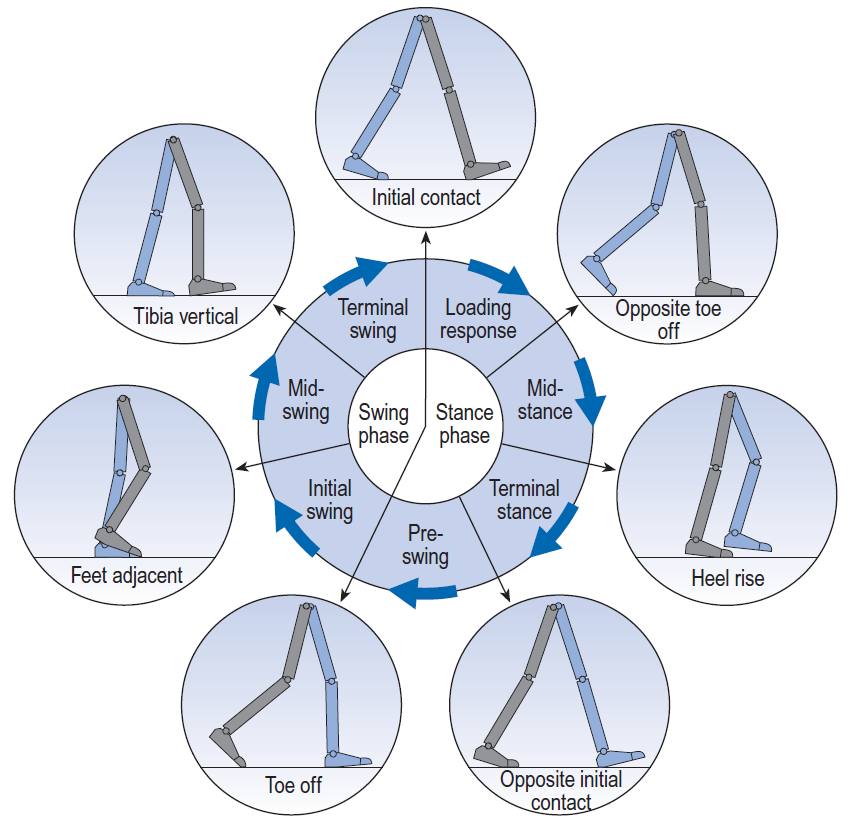
\includegraphics[scale=0.5]{figures/bProblemloesning/gang_cyklus2.png}
	\caption{Figurtekst… \fxnote{SKAL MODIFICERES. Gør så at figuren også har den procentvise fordeling af faserne på} \cite{VaughanDavisOConnor1992}}
	\label{fig:gang_cyklus}
\end{figure}
	
Det fremgår af billedet, at standfasen og svingfasen yderligere er inddelt henholdsvis i 5 og 3 faser. \newline
Standfasen første fase er et hæl-nedslag som starter hele cyklussen, idet der opnås kontakt med overfladen med den højre hæl. Herefter er foden flad og den venstre fod er derimod i berøring med overfladen med tåspidserne. Hælen på den højre fod løftes nu, alt i mens den venstre fod, som er i svingfasen, passerer den højre fod. Der opstår nu et hæl-slip for den højre fod, og der skabes en berøring af den venstre fod på underlaget. Standfasen afsluttes med en fleksion af anklen og dermed et afsæt fra tæerne på højre fod. \newline
Den højre fod, og det højre ben, er dermed i svingfasen, som påbegyndes med en acceleration af foden og benet. Denne acceleration begynder når foden ikke længere har kontakt med underlaget i standfasen. Derfor vil det højre ben blive bevæget frem mod det venstre ben. Efterfølgende vil der være et såkaldt, midt-sving som forekommer når højre fod er lige under kroppen og dermed ud for den venstre fod, som er i kontatkt med jorden. Afsluttende for svingfasen er der en deacceleration. Denne fase involverer en række muskler som sænker hastigheden af benet og fodens fremadgående bevægelse, således kroppen er klar til det kommende hæl-nedslag i standfasen.
	





\subsection{Løb}
Løb beskrives, ligesom gang, gennem forskellige faser. 
Løbecyklussen består af fire faser som vist på \figref{fig:loebecyklus}: standfasen, den første svævefase, svingfasen og den anden svævefase. \citep{Adelaar1986}

***Billede*** \label{fig:loebecyklus} \citep{Adelaar1986}

Den første fase, standfase, udgør 40\% af løbecyklussen og starter idet den højre hæl rammer jorden, derefter fortsættes foden til midt stand, og afslutningsvis afsættes der med tæerne, hvilket leder op til den næste fase, den første svævefase. Svævefasen, som går igen to gange i løbecyklussen, udgør hver 15\%, og er karakteriseret ved at begge ben er løftet fra jorden, hvorved de ikke er supportet. Mellem de to svævefaser, er svingfasen, som udgør 30\%. Denne fase initieres idet hælen hæves og knæet føres frem, hvorefter hælen igen sænkes, og svævefasen gentages, før en ny cyklus kan påbegyndes. \citep{Adelaar1986,Novacheck1998}

Længden af disse faser varierer dog alt efter hvor hurtigt man løber, da svævefasen øges. 

Løb er karakteriseret ved, at kun én fod rør jorden ad gangen. Dette resulterer i at der er et større stress på leddene ved løb i forhold til gang. Eksempelvis vil en person på 68 kg have et stress på sin fod på 35 kg/m ved gang, mens det ved løb vil være et stress på 110 ton/m. 















\section{Brugersikkerhed}
\textit{Nedenstående afsnit beskriver hvilke ricisi der kan forekomme når en bruger tilkobles elektronisk udstyr. Metoder hvorpå de omtalte risici kan forebygges, beskrives også. Afsnittet underbygges af det funktionelle krav, hermed at systemet skal været sikkert for brugeren at anvende.}

Medikoteknisk udstyr er tilsluttet en spændingsforsyning i form af eksempelvis strømnettet eller et batteri. Der indgår derfor en spænding og dermed en elektrisk strøm i det elektroniske kredsløb. En elektrisk fare kan opstå når brugeren er tilkoblet det medikotekniske udstyr, og kan dermed risikere at blive udsat for makro- og mikroshock fra hele det elektriske kredsløb. Makroshock er defineret som en elektrisk strøm, som løber igennem kroppen på den tilsluttede person. Denne strøm løber oven på huden, og er overfladisk. Mikroshock er defineret som elektrisk strøm, som løber igennem en persons væv deriblandt hjertet. Den elektriske størm som personen påvirkes med under mikroshock, medfører oftest en større potentiel fare end makroshock. \citep{Webster2011} \newline
Medikoteknisk udstyr har dermed en risiko for at påføre brugeren en strøm som potentielt kan være farlig. Det er derfor væsentligt, at det elektroniske udstyr involverer sikkerhedsmæssige elementer således risikoen for lækstrømme sænkes. Eksempelvis benyttes isolation og jordning som sikkerhedsmæssige procedurer, for at nedbringe risikoen for at tilføre brugeren lækstrømme i form af henholdsvis makroshock eller mikroshock. Isolation benyttes til at isolere brugeren fra elektriske spændingskilder i det medikotekniske udstyr. Ydermere benyttes jording som en sikkerhedsforanstaltning, idet alle aktive komponenter føres til jord, altså et fælles nulpunkt. De aktive komponenter er forbundet til jord, hvormed eventuelle lækstrømme vil løbe denne vej og dermed væk fra brugeren. \citep{Webster2011} \newline 
Eftersom systemet bliver forsynet med en lav spænding samtidig med at systemet være mobilt, vil der blive benyttet batterier som spændingskilde. Batterier kan dog være forbundet med enkelte sikkerhedsmæssige farer. Farerne kan opstå hvis batterierne ikke bliver brugt efter de foreskrevne regler for det pågældende batteri. Dette kan risikere at ødelægge batteriet, hvormed brugeren vil kunne blive udsat for forbrændinger som følge af fejlbrug af batteriet. Et ødelagt batteri kan ydermere risikere at medføre åndedrætsbesvær for brugeren. Disse farer kan undgås hvis man følger batteriets sikkerhedsanvisninger. \citep{NREL2011}


%  For at sikre lækstrømme ikke opnår en størrelse hvormed makro- og mikroshock kan være alvorligt skadelige, kan isolation benyttes. Ved isolation sikre man at det medikotekniske udstyr ikke er i direkte forbindelse med en betydelig spændingskilde. I og med at udstyret er forsynet med en lav spændingskilde, begrænses størrelsen af de lækstrømme som kan forekomme. Den anden sikkerhedsforanstaltning som kan implementeres for at gøre udstyret sikkert for brugeren er jording. Jording sikre at alle
\section{Hardware teori}
\textit{Følgende afsnit omhandler de teoretiske aspekter af systemets hardware. Grundlæggende teori for accelerometer, gyroskop og pulssensor beskrives med henblik på at kunne detektere og kategorisere de ønskede aktiviteter.}

\subsection{Accelerometer}
Et accelerometer er et elektromekanisk apparat, som anvendes til at måle accelerationskræfter, hvilket er ændringer i hastighed og position \citep{Goodrich2013,TittertonWeston2004}. Enheden for dette er $m/s^2$ eller $g$, hvor 1~g svarer til 9,82~$m/s^2$. Et accelerometer måler dermed egenaccelerationen af et givent objekt.\fxnote{En g-kraft på jorden svarer til tyngdekraften på 9,82~$m/s^2$, men varierer med elevation. Wiki har en god forklaring af dette, hvis man stadig er i tvivl.}~\citep{Sparkfun,TittertonWeston2004}

Et accelerometer måler to former for acceleration: statisk og dynamisk. De statiske kræfter er tyngdekraften i forhold til vinkelretningen af accelerometeret. De dynamiske kræfter beskriver retningen af accelerometerets bevægelse og dets vibrationer \citep{Sparkfun,Goodrich2013,Engineering}. Ydermere forefindes accelerometre med henholdsvis en, to eller tre måleakser. \citep{TittertonWeston2004} 

Accelerationen i et accelerometer beregnes ud fra Newtons anden lov, som ses i \eqref{eq:Newton}:
\begin{equation}\label{eq:Newton}
F~=~m \cdot a~=~m \cdot f~+~m \cdot g
\end{equation} 
I \eqref{eq:Newton} er den totale kraft (F) lig med den påvirkede masse (m) ganget med dets acceleration (a). Dette kan også defineres som massen (m) multipliceret med henholdsvis de eksterne kræfter (f) og tyngdekræften (g). \citep{TittertonWeston2004,Academic2016d} \newline
Illustrativt kan et accelerometer beskrives som en kapsel, hvori der er en indre masse spændt mellem to fjedre, hvilket illustreres på \figref{acc_simpelt}. En kræftpåvirkning kan skabe en ændring af den indre masses placering i den sensitive akse, hvormed accelerationen af selve accelerometeret i den pågældende akse kan beskrives. Hvis accelerometeret svæver i luften, vil både kapslen og den indre masse udelukkende påvirkes af tyngdekræften, og der vil derfor ikke registeres en acceleration.\citep{TittertonWeston2004,Academic2016d}
\begin{figure}[H]
	\centering
	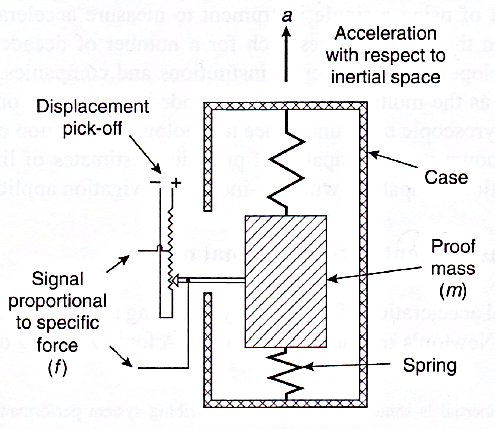
\includegraphics[scale=0.4]{figures/bProblemloesning/accelerometer_basic.png}
	\caption{På figuren ses opbygningen af et accelerometer med en indre masse, fjedre og den ydre kapsel. Det ses på den indre masse, at denne er forskubbet mod bunden af kapslen, grundet en acceleration af accelerometeret. \citep{TittertonWeston2004} (Modificeret)}
	\label{acc_simpelt}
\end{figure}\vspace{-.25cm}
Et stillestående accelerometer påvirkes altid af $\pm$1~g på en bestemt akse afhængig af sensorens orientering. Eksempelvis, hvis accelerometeret er placeret på et bord med dets positive y-akse i vertikal retning, da vil y-aksen blive påvirket med +1 g. I dette tilfælde vil de andre akser, henholdsvis x- og z-aksen, ikke blive påvirket af nogen kræfter. \citep{Serway2010}

Accelerometre benyttes enten i en åben eller lukket kreds. I en åben kreds fastholdes den indre masse til et nulpunkt ved at være udspændt mellem to fjedre. Ved acceleration af den ydre kapsel bevæges den indre masse væk fra nulpunktet, hvorved ændringen for et enkelt akset accelerometer vil være proportional med kræften, som påvirker systemet. \newline
I en lukket kreds fastholdes den indre masse til et nulpunkt ved hjælp af magnetiske kræfter. Oftest påmonteres en spole på den indre masse, hvormed magnetfeltet forstærkes. Det er muligt at foretage mere præcise målinger omkring nulpunktet end ved en åben kreds. Accelerometre med den lukkede kreds er derfor mere præcis end accelerometre med en åben kreds. \citep{Serway2010,TittertonWeston2004,Academic2016d}
\subsection{Gyroskop}
Et gyroskop er et elektromekanisk apparat, som anvendes til at måle omdrejninger per sekund eller vinkelhastighed om en given akse, hvilket illustreres på \figref{fig:gyro}. Enhederne på data fra et gyroskop er henholdsvis revolutions per second (RPS) og $^\circ$/sekund. \newline
Et gyropskop kan give information om orienteringen eller navigationen af objektet, som sensoren optager data fra. Hvis et gyroskop eksempelvis drejes én omgang om egen akse i sekundet, vil den registrere en vinkelhastighed på 360 grader pr sekund. \citep{Sparkfun_gyro,Barbour2014}
\begin{figure}[H]
	\centering
	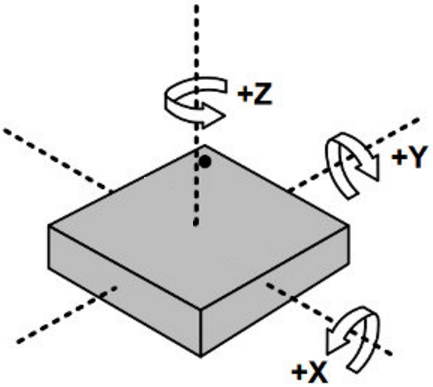
\includegraphics[scale=0.6]{figures/bProblemloesning/gyro.png}
	\caption{På figuren ses et gyroskops måling af rotation omkring x-, y- og z-aksen. \citep{Sparkfun_gyro} (Modificeret)}
	\label{fig:gyro}
\end{figure}

Alt afhængigt af formålet med at benyttes et gyroskop, findes der en række forskellige gyroskoper heriblandt vibrations-, elektrostatiske- og kernemagnetisk resonans gyroskoper. \citep{LuingeVeltink2005,TittertonWeston2004} Et gyroskop kan for eksempel registrere vinkelhastighed ved at anvende tyngdekræften og en lille indre masse \citep{Sparkfun_gyro,Barbour2014}. Hvis et gyroskop eksempelvis opsamler data ved cykling, mens det er placeret proximalt for den laterale malleolus, vil massen blive udsat for en roterende bevægelse omkring den horisontale akse. Massen vil blive henholdsvis tungere og lettere i processen på grund af ydre påvirkende kræfter, hvorfor outputtet vil komme til udtryk som en sinus-bølge. Outputtet er afhængig af tyngdekræftens påvirkning af massen, hvorfor et varierende output kræver en bevægelse.% Gyroskopet vil, uafhængigt af placering, have et fast output, som det vil vende tilbage til efter en bevægelse.
%Et gyroskop fungere ved at anvende inerti egenskaberne der opstår når et hjul spindes med en høj hastighed. Ved at hjulet fastholder den samme retning omkring aksen, kan impulsmomentmomentet, dets inertiprodukt samt hastighed være med til at definere en referenceretning. 
%De fundementale principper bag virkningen af et gyroskop er blandt andet det gyroskopiske inerti, som er når hjulet drejer om sin egen akse og står vinkelret på aksen. impulsmomentet som er fordelingen af en masse på et rotor, hvor vinkelhastigheden også har en betydning, og præcession som er rotationen omkring egen akse. 
%De signaler som opfanges af et accelerometrer, inkluderer ikke signaler fra den roterende akse og derfor kan en præcis orientering ikke opfanges. For at forbedre nøjagtigheden, kan man anvende gyroskoper som et supplement til accelerometre .
%Et gyroskop måler vinkelhastighed, hvor ændringen i orientering kan måles ved at integrere vinkelhastigheden på baggrund af en algoritme. \citep{LuingeVeltink2005}
%
\subsection{Sammenligning af accelerometer og gyroskop}
Et acceleromteter er i stand til at måle accelerationen af et objekt, eksempelvis bevægelsen af et ben under gang og løb. Dette er muligt da denne sensor måler den kraft som eksempelvis et ben påvirkes med, ved en given bevægelse. Denne kraft vil medføre karakteristiske udsving for den givne bevægele. Særligt gang og løb har en karakteristisk påvirkning på kroppen vedrørende acceleration. Accelerometeret vil derfor være fordelagtigt at benytte til en registrering af gang og løb, da det er muligt at genkende og bestemme betydningen af disse karakteristika. Gyroskopet registrerer rotationen af et objekt om en given akse. Med antagelse om ideelle forhold vil det derfor være fordelagtigt at benytte et gyroskop til registrering af cykling, idet denne bevægelse overordnet set er en cirkulær bevægelse omkring én akse. Betydningen heraf. vil medføre at cykling tilnærmelsesvis kan afspejles som en sinus bølge med varierende frekvens alt efter hastighed. 

%\textbf{Gammelt forslag} \newline
%Den væsentligste forskel er, at et gyroskop kan måle rotation, hvilket et accelerometer ikke er i stand til. Accelerometret er fordelagtigt at bruge til at måle orientering af et stationært punkt i forhold til jordens overflade men under bevægelse bliver outputtet mere komplekst. For eksempel vil et accelerometer under frit fald vise 0. \citep{Goodrich2013,TittertonWeston2004,LuingeVeltink2005} \\
%Et gyroskop reagerer ikke på vibration eller støj, hvilket et accelerometer kan opsamle som støj på signalet. Derudover reagerer et gyroskop hurtigt men dets output for hældningsvinkel vil blive mere ukorrekt over tid grundet usikkerhed i de enkelte målinger, hvorfor den akkumulerede vinkel ligeledes bliver mere ukorrekt. Et accelerometers respons er langsommere men mere præcis over tid. Igennem kalibrering, hvor hvert apparat assisterer til kalibreringen af den anden, vil de tilsammen kunne holdes korrekt på kort og lang sigt. \citep{Barbour2014,Brasca2011}
\subsection{Pulssensorer}
Kroppens puls kan detekteres på en række forskellige måder, eksempelvis elektrisk eller optisk.
Elektriske pulssensorer, måler pulsen ved hjælp af en elektrisk kontaktflade mellem sensor og person, hvilket skabes ved hjælp af elektroder. Pulsen detekteres af de elektriske pulssensorer, som forskelle i den elektriske ladning. Udfaldet af målingerne kan være afvigende, da individuelle faktorer såsom en personens blod, svedniveau eller hudfedt er en afgørende faktor. For at minimere disse udfald kræves der en god elektronisk kontakt, heraf er præparering af huden nødvendig. Denne type plusmåling kræver en placering ved hjertets afledninger\fxnote{Kig her for at se hjertets afledninger: https://www.sundhed.dk/borger/sygdomme-a-aa/hjerte-og-blodkar/illustrationer/tegning/placering-af-ekg-elektroder/}. \citep{PhuaLissorguesMercier2009}  \\
Optiske pulssensorer registrerer puls ved hjælp af lysindhold. En LED udsender en lyskilde som passerer huden og en blodåre, hvoraf en mængde af dette lys absorberes af hæmoglobin i blodet. Efterfulgt af dette opfanger en fotodiode mængden af det resterende lys. Størrelsen af dette lys er den bestemmende faktor vedrørende mængde af blod i blodåren, og er heraf omvendt proportionalt. Pulssensoreren udsender positive udsalg på signalet, desto mere blod der registreres. Denne type sensor placeres derfor over en blodåre.\citep{PhuaLissorguesMercier2009,SrinivasReddySrinivas2006} 

%\subsubsection{Registrering af puls}
%Pulsen er angivet som forskellen i det systoliske og diastoliske blodtryk som slag per minut. Pulsen kan måles manuelt ved at placere to fingre over en arterie, og derefter tælle hvor mange slag der er i minuttet. Hyppigst måles pulsen fra radial arterien på håndleddet eller på halsen, men enhver arterie der kan mærkes, kan bruges til at måle pulsen ved, se \figref{pulsmaaling}. \citep{CNX2016}
%
%\begin{figure}[H]
%	\centering
%	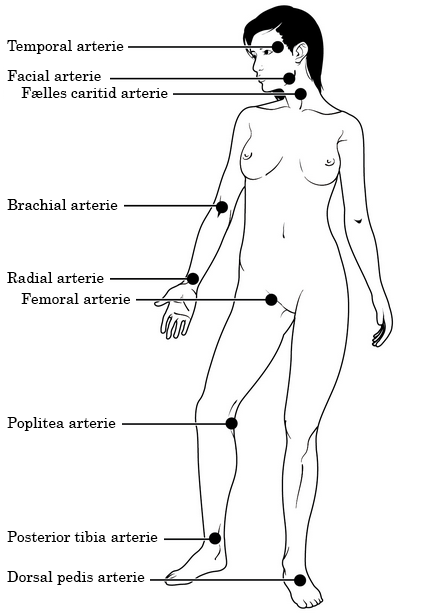
\includegraphics[scale=0.6]{figures/bProblemloesning/puls.png}
%	\caption{På figuren ses steder det er muligt at måle puls.\citep{CNX2016}}
%	\label{fig:sensor_placering}
%	\end{figure}
	



\section{Digital Teori}
Til dette projekt anvendes CY8CKIT-043 Programmable System on Chip (PSoC) 4 M-Series Prototyping Kit, CY8CKIT-042-BLE Bluetooth® Low Energy (BLE) Pioneer Kit og programmet PSoC Creater i den digitale del til at opsamle det biologiske signal.\\
CY8CKIT-043 PSoC 4 M-Series Prototyping Kit er en prototyping platform, der indeholder tre Advanced RISC\fxnote{REDUCED INSTRUCTION SET COMPUTER - RISK kan load/store og har pipelinable instructions, hbvilket betyder, at vi ikke behøver vente på, at en instruktion bliver færdig før vi starter med den næste. Fetch - decode - exicude, laver mere på samme tid. (kilde - slide første forelæsning)} Machines (ARM) mikroprocessorer, hvilket ses på \figref. Den første ARM cortex-M3 baserede PSoC på mikrokontrolleren kan indeholde programmer, der kan indlæses på en computer ved hjælp af USB stikket. Den bruges til at programmere og debug softwaren på programmeringsdelen af mikrokontrolleren, hvorfor denne del kan knækkes af resten af stikket og fungere selvstændigt. Dette kræver dog, at softwaren først er programmeret på den anden mikroprocessorer, som er ARM cortex-M0 baserede PSoC. Denne fungerer som hovedcomputeren, der programmeres på igennem c koden. På bagsiden af mikrokontrolleren sidder ARM coretex-m0 BLE Programmable Radio on Chip (PRoC), hvilket ikke vil blive benyttet i dette projekt.\fxnote{Denne ARM har ikke lige så mange muligheder for afbenyttelse,  da BLE fylder så meget, så der er ikke plads til meget andet.} \citep{CYPRESS2016PSoC,Semiconductor2016}
\begin{figure}[H]
	\centering
	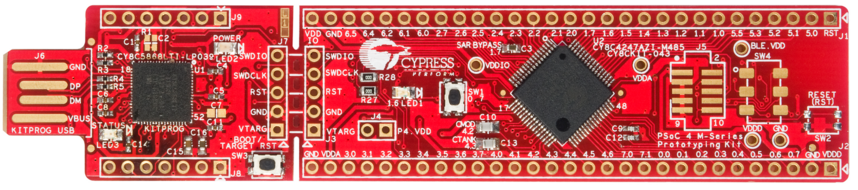
\includegraphics[scale=0.5]{figures/dProblemloesning/PSoC.PNG}
	\caption{På figuren ses mikrokontrolleren CY8CKIT-043 PSoC 4 M-Series Prototyping Kit. \citep{CYPRESS2016PSoC}}
	\label{fig:PSoC}
\end{figure}
Denne prototyping Kit platform er ved hjælp af en computer med aktiv bluetooth i stand til at sende og modtage trådløs data fra Y8CKIT-042-BLE Bluetooth® Low Energy (BLE) Pioneer Kit platformen, som indeholder en PRoC.
%CYPRESS2016BLE
%CYPRESS2016PSoC
%Semiconductor2016
%Semiconductor2016BLE
\subsection{Universal Asynchronous Receiver Transmitter(UART)}
En UART er et led mellem et parallelt og serielt interface, der både modtager data (RX) og sender data (TX). Dataen sendes som bit, og kan både sendes serielt eller parallelt.\citep{Jimb02016a}\newline 
Parallelt bliver flere bit overført på samme tid, hvormed et 8-bit system har 8 ledninger hvor der i den ene ende er en RX kobling og den anden er TX kobling.\citep{Jimb02016a}\newline
Den serielle kommunikation foregår asynkront, og kan foregå med ned til én ledning, da kun en bit overføres af gangen. Det er nødvendigt at sætte en baudrate, da TX sender i forhold til denne og RX sampler i forhold til den forventede baudrate\fxnote{baudrate = Hvor hurtigt der sendes data (bits per sekund[bps])}. Det modtagne data gemmes ofte i en buffer, som efterfølgende videregives i form af firs-in-first-out (FIFO) princippet.\citep{Jimb02016a,Chun-zhiYin-shuiLun-yao2011}\newline 
Overførsel af data sker asynkront, som det ses på \figref{fig:asynkron}. Ved denne kommunikationsform opererer RX og TX ved to forskellige klokker. For at kunne lave dataen synkront, sættes et startbit og et stopbit. UARTens opgave er at læse data fra FIFO parallel data, som laves om til seriel data. Denne data kan sendes til andre enheder. Når RX i en anden enhed modtager en startbit, laves data om fra seriel til parallel data, hvorefter data kan skrives til modtager-FIFO.\citep{Jimb02016a,Chun-zhiYin-shuiLun-yao2011} 

\begin{figure}[H]
	\centering
	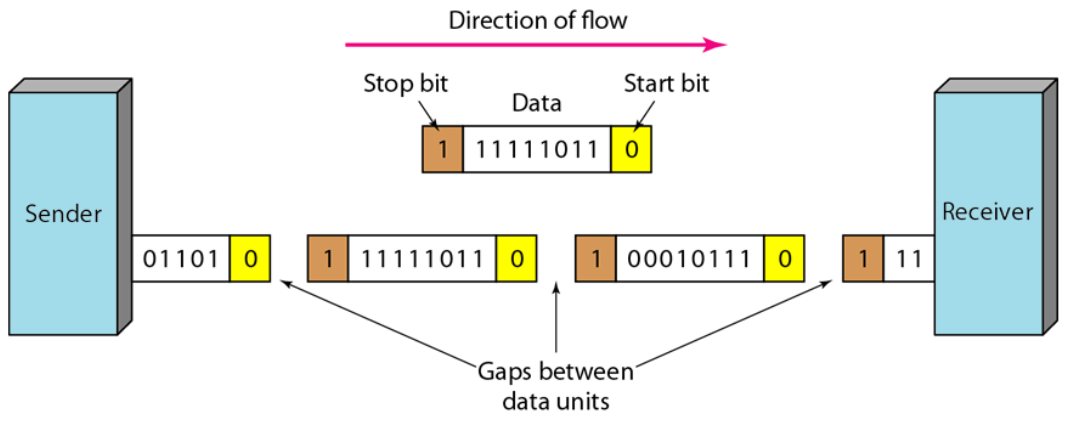
\includegraphics[scale=0.6]{figures/bProblemloesning/asynkron.png}
	\caption{På figuren ses asynkron dataoverførsel.\citep{Sharma2016}}
	\label{fig:asynkron}
\end{figure}

Nogle enheder indeholder mere end en seriel-linje, og kan enten fungere som fuld-duplex eller halv-duplex. De enheder der er fuld-duplex, kan både sende og modtage data på samme tid. Ved halv-duplex, skal dette foregå på skift.\citep{Jimb02016a}
\input{rapportAfsnit/dProblemloesning/Power_mode}
\subsection{Digitale filtre}
%Digitale filtre kan opnå tusinde gange bedre resultat end analoge filtre.

Digitale filtre benyttes grundlæggende til to formål; adskillelse og genskabelse af signaler. Signaladskillelse %benyttes til at adskille signaler fra hinanden, hvilket ofte 
benyttes ofte i forbindelse med at filtrere støj fra det ønskede signal.\fxnote{eksempelvis ved ekg eller hjertelyd, hvor vejrtrækning og andre kropssignaler/lyde skal fjernes} Signalgenskabelse benyttes, hvis signalet er blevet beskadiget eller forvrænget. \fxnote{eksempelvis ved rystelser hvis måleudstyret er dårligt eller hvis ikke vi får sat den ordentlig fast på forsøgspersonen.} \citep{Smith1997}

Ethvert lineært filter har en impulsrespons, steprespons og en frekvensrespons. Disse responser indeholder information om filteret på forskellig vis og giver tilsammen information om, hvordan filteret vil agerer i givne situationer.\fxnote{hvis en af disse er oplyst eller defineret for filteret, kan de to andre udregnes matematisk.} \citep{Smith1997} Et filter designes ud fra dets responser. Den mest ligetil metode kaldes filterkernen eller Finite Impulse Response (FIR) filtre, hvor signalets inputs summeres med filterets impulsrespons. En anden metode kaldes et rekursivt filter eller Infinite Impulse Response (IIR) filtre, hvor tidligere outputværdier benyttes sammen med inputtet. For at finde impulsresponsen for et rekursivt filter, indsendes en impuls som input i filtret, og impulsresponsen er outputtet. Denne impulsrespons består af en sum af sinuser, som eksponentielt falder i amplitude. Dette resulterer i, at impulsresponsen bliver uendelig lang. \citep{Smith1997,Blandford2013} \newline
Et filter kan derudover designes ved, at filtrets steprespons eller frekvensrespons sammenholdes med sin impulsrespons. Stepresponsen er integralet af impulsresponsen, som kan findes ved at indsende en stepbølge i filteret. Outputtet heraf vil være stepresponsen. Frekvensresponsen kan findes ved at finde den diskrete Fourier transformationen (DFT) eller Fast Fourier transformationen (FFT) af impulsresponsen. \citep{Smith1997} %Resultatet af filterdesignet er typisk en overføringsfunktion i z-donæmet\fxnote{frekvensdomænet}. Ud fra denne kan filteret analyseres med henblik på at bestemme impulsresponsen, filterets stabilitet, steady-state frekvensrespons, differensformlen og responsen til et arbitrært input. \citep{Blandford2013} %I designfasen for filtre, startes der med at blive set på signalets frekvensspektrum, hvorved det vælges om der er behov for et lavpas-, højpas-, båndstop- eller båndpasfilter, og hertil også knækfrekvenserne for dem. Ud fra signalets frekvens, vælges også samplingshastigheden i henhold til Nyquist\fxnote{2 gange signalets frekvens}. Herefter vælges hvilken filtertype der egner sig bedst til systemet. \citep{Blandford2013}

\subsubsection{Finite Impulse Response filtre}
FIR filtre er defineret som digitale filtre med et endeligt antal impulsresponser. Det vil sige, at filteret har en impulsrespons med et endeligt antal ikke-nulværdier\fxnote{nonzeros}, hvorfor filtret kan designes stabilt og med en lineær fase. \citep{Blandford2013} Det fremgår af den generelle formel for FIR filtre, som ses i \eqref{eq:fir}, at filteret benytter tidligere og nutidige inputs. Dette er den afgørende faktor for, at responsen har et endeligt antal impulsresponser. 
\space
\begin{flalign}
	Y[n] = \sum_{m=0}^{m} b_m X[n-m]
	\label{eq:fir}
\end{flalign}
\space
FIR filtre inddeles i fire typer impulsresponsfunktioner, som det ses på \figref{fig:FIR_typer}. Type 1 har en lige orden og ulige længde, hvilket medfører, at responsen er centreret omkring den midterste impuls. Denne type er symmetrisk, hvorfor hele impulsresponsen ligger på den samme side af x-aksen. Type 2 er ligeledes symmetrisk, men har en ulige orden og lige længde. Dette resulterer i, at responsen er centreret imellem de to midterste impulser. %Disse kan skrives som en sum af cosinus funktioner.
Type 3 har en lige orden og ulige længde men er asymmetrisk, hvilket %i modsætning til type 1 og 2, 
gør at impulsresponsen ligger på begge sider af x-aksen. Type 4 har %, ligeledes med type 2, 
en ulige orden og lige længde, men er også asymmetrisk. %Disse kan skrives som en sum af sinus funktioner.
\citep{Blandford2013} \newline

\begin{figure}[H]
	\centering
	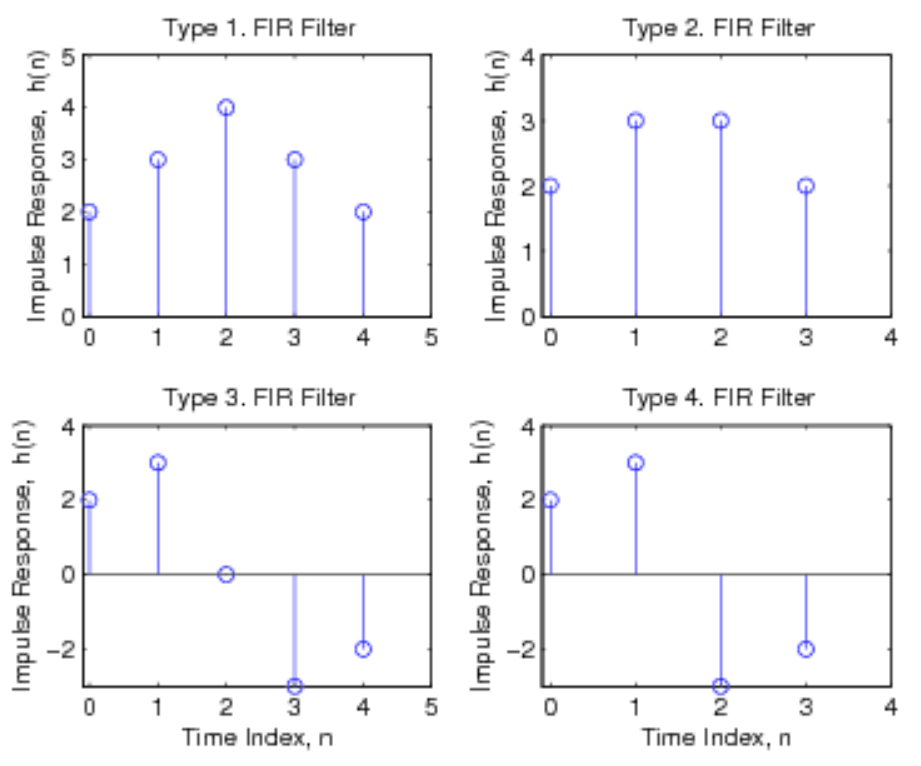
\includegraphics[scale=0.6]{figures/bProblemloesning/FIR_type.png}
	\caption{På figuren ses de fire typer af FIR filtre der findes. \citep{Burrus2016}}
	\label{fig:FIR_typer}
\end{figure}

De forskellige impulsresponsfunktioner benyttes til valg af filtertype, hvor det vurderes, hvilke der egner sig bedst til formålet. De forskellige konfigurationer skal tage højde for, om der ønskes et lavpas-, højpas-, båndpas- eller båndstopfilter. \citep{Blandford2013} \newline
FIR filtre optræder ligeledes som forskellige konfigurationer, heriblandt Parks-McClellan algoritmen, frekvens sampling, window type og moving average. \citep{Blandford2013}
%
%Windowing:
%Når der benyttes Fourier serier til at lave et ideelt FIR filter, fås en række koefficienter mellem minus uendelig og plus uendelig. Da et uendelig langt filter ikke kan implementeres, forkortes antallet af koefficienter til et antal som kan implementeres og stadig tilnærmelsesvis giver et ideelt filter. Matematisk sker dette ved at gange impulsresponsen med et rektangulært window. 
%
%Diskret fourier transformation (DFT) af et rektangulært window i tidsdomænet, giver en sinusfunktion i frekvensdomænet.
%
%\begin{flalign}
%Y[n] = H*W = \sum_{k=0}^{\infty} H[k] \cdot W[n-k]
%\label{eq:window}
%\end{flalign}
%
%
%Derudover kan filtrene implementeres på forskellig vis, alt efter deres formål. Moving average filtre benyttes til at udglatte signalet, ved at finde gennemsnitsværdien for et bestemt antal samples. Herved får en eventuel støj får mindre betydning for signalets udformning.
%
%\begin{flalign}
%	avg = \frac{1}{N} \sum_{i=1}^{N} x_i
%	\label{eq:mavg}
%\end{flalign}


\subsubsection{Infinite Impulse Response filtre}
Et IIR filter er, modsat FIR filtre, defineret som et digitalt filter med uendelig mange impulsresponser. Derfor har dette filter en impulsrespons med uendeligt mange nulværdier\fxnote{zeros}, hvilket gør at filterets impulsresponsen falder eksponentielt i amplitude og resulterer i en uendelig respons. Filteret kan derfor kun tilnærmelsesvis designes med en lineær fase, hvorfor det kan risikere at være ustabilt. Idet IIR filtre benytter tidligere outputs, er det et feedback filter, hvilket gør det udregningseffektivt.\fxnote{nemmere at udregne} \citep{Blandford2013} Af den generelle formel for IIR filtre i \eqref{eq:iir} fremgår det, at filteret benytter tidligere og nutidige inputs men også tidligere outputs, hvormed det får uendeligt mange impulsresponser. 
\space
\begin{flalign}
	Y[n] = \sum_{k=1}^{k} a_k Y[n-k] + \sum_{m=0}^{m} b_m X[n-m]
	\label{eq:iir}
\end{flalign}
\space 
IIR filtre optræder som forskellige filterkonfigurationer, heriblandt Butterworth, Chebyshev og elliptisk. Disse kan alle benyttes til lavpas-, højpas-, båndpas- eller båndstopfilter og designes ud fra krav om ripples, linearitet, dæmpningsgrad og faseforskydelse. \citep{Blandford2013}
\section{Opsamling af pilotforsøg}
Igennem pilotforsøget, som ses i \appref{pilot}, blev aktiviteterne gang, løb og cykling undersøgt og behandlet. Databehandlingen heraf tog udgangspunkt i pilotforsøgets formål, hvormed fortolkningen af dette er pilotforsøgets essens. \\
Tre mulige placeringer af en aktivitetsmåler blev undersøgt for alle aktiviteter. Resultatet af dette medførte at aktiviteternes signalamplituder for henholdsvis accelerometer og gyroskop, blev undersøgt. Placering A blev valgt, hvorigennem accelerometeret bør have et arbejdsområde på $\pm$16 g, og gyroskopet på minimum 320,5 dps. \\
Aktiviteterne blev undersøgt med henblik på hvorvidt en mulig adskillelse af disse var mulige. Resultatet af dette medførte, at fælles for gang og løb forekom signal events på accelerometerets y-akse, hvorigennem aktiviteterne antageligvis kan adskilles. Karakteristika vedrørende cykling blev undersøgt med henhold til gyroskopets z-akse. Resultatet heraf medførte et tydeligt sinus lignende signal. Det antages at et sådan signal skaber mulighed for detektering. Det blev ydermere sikret at signaler fra gang og løb ikke havde en sinus lignende tendens vedrørende gyroskopets z-akse, hvoraf adskillelse ligeledes antages at være mulig. \\
Aktiviteternes frekvensindhold blev ligeledes undersøgt med henblik på at kunne fastsætte systemets samplingsfrekvens, samt knækfrekvens for eventuelle filtre. Resultatet heraf er at det største frekvensspektrum for gang og løb befinder sig op til 45 Hz, og cykling op til 6 Hz. 


\section{Kravspecifikationer}
\textit{I det følgende afsnit opstilles krav samt tolerancer hertil for hver del i det samlede system. Det sikres herved, at hver enhed kan fungere efter hensigten.}

Formålet med aktivitetsmåleren er at kunne registrere og adskille aktivitetsformerne gang, løb og cykling. Aktivitetsmåleren vil dermed indeholde hardware og software, som tilsammen kan opsamle analoge signaler og udføre digital signalbehandling herpå. Det samlede system skal have et potentiale til at opfylde de funktionelle krav for systemet, beskrevet i \secref{funktionellekrav}. Endvidere vil nedenstående kravspecifikationer tage udgangspunkt i de opnåede resultater fra de udførte pilotforsøg, som er beskrevet i \appref{pilot}.
%
%\subsection{Krav til hardware}
%Aktivitetsmålerens hardware består af to sensorer, spændingsforsyning og en ADC. Disse elementer benyttes til en signalopsamling og -konvertering, hvoraf det digitale signal efterfølgende bliver behandlet af aktivitetsmålerens software.

\subsection{Spændingsforsyning}
MCU'en kræver en spændingsforsyning for at kunne fungere, hvilket enten kan ske igennem USB porten eller tilføres fra en mobil enhed. Spændingsforsyningen skal kunne forsyne MCU'en i en hel dag samt være sikkert for brugeren. %Det samlede system skal benytte elektroniske komponenter, hvorfor en spændingsforsyning er nødvendig. Spændingsforsyningen skal tage hensyn til mobilitet samt brugersikkerhed.

\textbf{Krav til spændingsforsyning} \newline 
Spændingsforsyningen skal:
\begin{itemize}
	\item Levere mindst 1,71 V og maks 5,5 V til MCU'en\fxnote{Alle mikroprocessorer kræver 1,71-5,5 V for at kunne fungere, selvom der står 3,3-5,5 V i databladet for mikroprocessoren.}. Der accepteres ikke en spænding under minimumsgrænsen eller over maksimumsgrænsen. %en tilstrækkelig spænding til alle systemets aktive komponenter, og må varierer med $\pm$5\%.
	\item Være i stand til at levere denne spænding i mindst 15 timer. Der accepteres ikke, at spændingsforsyningen leverer under 1,71 V eller over 5,5 V i mindre end 15 timer.
	%\item Muliggøre spændingsopsætning af systemet udenom elnettet og	være elektrisk sikkert.
	\item Være mobil og dermed besidde en opsætning udenom elnettet, hvilket gør systemet mere elektrisk sikkert. Der accepteres ikke, at systemet skal kobles til elnettet og derved ikke være mobilt.
\end{itemize}

\subsection{Mikrokontroller}
Vi har fået udleveret en specifik MCU, som skal benyttes til projektet. Der kan derfor ikke stilles krav til selve hardwaren hertil. Dog skal MCU'en fungere som spændingsforsyning til IC samt pulssensor, hvorfor der skal stilles krav hertil. I \secref{sec_design_LSM9DS1} og \secref{sec_design_puls} beskrives de specifikke sensorer for dette projekt, hvorfor spændingsforsyningen hertil er bestemt.

\textbf{Krav til mikrokontrolleren} \newline 
Mikrokontrolleren skal:
\begin{itemize}
	\item Levere 3,3 V til IC'en. Der accepteres en afvigelse på 5\%.
	\item Levere mellem 3 V og 5 V til pulssensoren. Der accepteres ikke, at pulssensoren modtager en spænding under minimumsgrænsen eller over maksimumsgrænsen.
\end{itemize}

\subsection{Accelerometer}
% Et accelerometer kræver en given spænding for at kunne optage data. Accelerometret i  LSM9DS1 kræver 3,3 V for at være operativt. %Sensoren skal være i stand til at optage data ved tilførslen af en DC spænding med baggrund i spændingsforsyningens krav. Arbejdsområdet for et accelerometer er angivet i g, og er derfor påvirkelig overfor den accelerationen som sensoreren udsættes for. Den påvirkning som udøves på sensoren er dermed afhængig af flere faktorer såsom vægt, bevægelsens hastighed og bevægelsens mønster. \newline
Pilotforsøget viste en maksimal acceleration på +16,95 g og -8,83 g. Den maksimale positive g værdi antages derfor som værende den største acceleration, som accelerometret vil blive påvirket af som prototype. Dog er pilotforsøget udført på en forsøgspopulation (n=4) med voksne mennesker. Det antages derfor, at den gennemsnitlige vægt er større end målgruppens, hvorfor et barn ikke vil kunne påvirke accelerometret med over 16 g. %Jævnfør pilotforsøget blev den optimale placering af sensorer med henblik på målgruppen bestemt. Placeringen af sensorer skal derfor være ud for den laterale malleolus.

\textbf{Krav til accelerometer} \newline 
Accelerometeret skal:
\begin{itemize}
%\item Være operativ ved 3,3 V fra MCU'ens VDD output spænding.\fxnote{Outputspændingen fra MCU'en er omkring 4.8V, men det afhænger måske er, hvilken spænding den får tilført? Ellers skal det reguleres med potentiometer} Der accepteres en afvigelse på +5\%.
\item Have et arbejdsområde på $\pm$16 g. Der accepteres ikke, at accelerometret har at arbejdsområde på under $\pm$16 g.
\end{itemize}

\subsection{Gyroskop} 
%Et gyroskop kræver en given spænding for at kunne optage data. Gyroskopet i  LSM9DS1 kræver 3,3 V for at være operativt. %Sensoren skal være i stand til at optage data ved tilførslen af en DC spænding med baggrund i spændingsforsyningens krav.
Det maksimale arbejdsområde for gyroskopet blev undersøgt i pilotforsøget, der udledte $\pm$160 dps som maksimalværdierne. Dette blev bestemt for en given frekvens ved cykling, hvorfor gyroskopet bør have et større arbejdsområde for at tage forbehold for en højere frekvens. % af omdrejninger på cyklen . Jævnfør pilotforsøget blev den optimale placering af sensorer med henblik på målgruppen bestemt.

\textbf{Krav til gyroskop} \newline
Gyroskopet skal:
\begin{itemize}
%\item Være operativ ved 3,3 V fra MCU'ens VDD output spænding.\fxnote{Outputspændingen fra MCU'en er omkring 4.8V, men det afhænger måske er, hvilken spænding den fårr tilført? Ellers skal det reguleres med potentiometer} Der accepteres en afvigelse på +5\%.
\item Have et arbejdsområde på x.
\end{itemize}

\subsection{Pulssensor}
En pulssensor kræver en given spænding for at kunne optage data, som tilføres fra MCU'en. Sensoren skal være i stand til at optage data ved tilførslen af en DC spænding. % med baggrund i spændingsforsyningens krav. 
Yderligere skal pulssensoren kunne opfange brugerens puls, med henblik på at bestemme intensiteten af den pågældende aktivitet.

\textbf{Krav til pulssensor} \newline
Pulsmåleren skal:
\begin{itemize}
%\item Være operativ mellem 3 V og 5 V. Der accepteres ikke, at pulssensoren modtager en spænding under minimumsgrænsen eller over maksimumsgrænsen.\fxnote{MCU'en leverer ca. 4,6 V fra sin VDD output}% eller ikke er funktionel i dette spændingsinterval.
\item Kunne opfange brugerens puls under fysisk aktivitet. Der accepteres ikke, at pulssensoren opfanger ukorrekt eller ikke tydelig puls under fysisk aktivitet.
\end{itemize}

\subsection{Analog-to-Digital Converter}
%Pilotforsøget undersøgte frekvensområdet for de pågældende aktiviteter, i forhold til de sensorer som er påtænkt til at detektere den givne aktivitet.\newline
Accelerometret i LSM9DS1 skal benyttes til at opfange gang, mens gyroskopet i LSM9DS1 skal benyttes til at opfange cykling. For at begge sensorer skal være i stand til dette, er det essentielt at vide det analoge signals frekvensområde. %Accelerometeret skal benyttes til at detektere gang og løb, hvorfor pilotforsøg blev undersøgt med henhold til frekvensområdet heraf. 
Pilotforsøget viste, at frekvensområdet for signalet ved gang og løb er 45 Hz, når det optages af et accelerometer. Ifølge Nyquist skal aktivitetsmålerens ADC derfor have en samlingshastighed, der er dobbelt så stor som det maksimale frekvensområde, men i praksis 10 gange større. Derfor skal ADC'en sample besidde en samplingshastighed på mindst 450 Hz for accelerometret. Det kan dog være fordelagtig at oversample. Dette giver mindre støj på signalet, da Nyquist frekvensen derved rykkes og fjerner aliasing. \newline
Frekvensområdet for signalet under cykling ved benyttelse af gyroskop blev under pilotforsøget undersøgt. Det fremgik heraf, at det maksimale frekvensområde var 6 Hz. Derfor skal ADC'en sample gyroskopets data med mindst 60 Hz.

\textbf{Krav til ADC} \newline
ADC'en skal:
\begin{itemize}
\item Sample accelerometerets output med mindst 450 Hz. Der accepteres ikke en samplingsfrekvens under denne værdi.
\item Sample gyroskopets output med mindst 60 Hz. Der accepteres ikke en samplingsfrekvens under denne værdi.
\item Repræsentere det analoge signal med maksimalt 5\% afvigelse. 
\end{itemize}
%
%\subsection{Krav til software}
%Aktivitetsmålerens software består af algoritmedesign til MCU'ens mikroprocessorer 4200M og EZ-BLE PRoC på henholdsvis GAB central og GAB peripheral, hvilket giver fire algoritmedesigns. Derudover skal disse to enheder kommunikere med hinanden, og en GUI designes for at give brugeren en visualisering af det behandlede data.

\subsection{Algoritmedesign}
Designet af de fire algoritmer ligger til grund for hele funktionaliteten af systemet. \\
Algoritmen på PSoC 4200M på den mobile MCU skal overordnet designes til at gøre hele MCU'en til en GAB peripheral. Den skal indeholde elementer, som henvender sig til IC'en, da gyroskopet skal deaktiveres hvis ikke i brug. Hvert tiende sekund skal algoritmen få gyroskopet aktiveret, som skal tracke om aktiviteten er cykling. Hvis ikke skal gyroskopet deaktiveres igen og spørges igen om 10 sekunder. Desuden skal algoritmen aktivere ADC'en, således signalerne af IC'en kan modtages. Algoritmen skal gøre mikroprocessoren i stand til at kunne detektere, om den pågældende aktivitet er gang, løb eller cykling. Tiden, som brugeren bruger på den pågældende aktivitet, samt pulsmålingen skal gemmes. Hvert kvarter skal algoritmen vække EZ-BLE PRoC fra power moden stop og den gemte data overføres hertil via UART kommunikation.\\
Algoritmen til EZ-BLE PRoC på GAB peripheral skal sørge for, at enheden er i power moden stop med mindre, at den modtager et interrupt fra PSoC 4200M på samme enhed. Når dette interrupt modtages, skal EZ-BLE PRoC modtage al data og overføre til en anden EZ-BLE PRoC på GAB central via BLE. \\
Algoritmen på EZ-BLE PRoC på GAB central skal få enheden til at modtage data fra EZ-BLE PRoC på GAB peripheral. Denne data skal sendes til PSoC 4200M på GAB central via UART kommunikation. \\
Algoritmen til PSoC 4200M på enheden tilkoblet en PC skal overordnet designes til at gøre hele MCU'en til en GAB central. Desuden skal algoritmen gøre, at mikroprocessoren kan modtage data fra EZ-BLE PRoC på GAB central og videreføre dette til en GUI på en PC via USB porten.

\textbf{Krav til algoritmedesign} \newline 
Algoritmedesignet skal:
\begin{itemize}
	\item Gøre PSoC 4200M på GAB peripheral i stand til at sample signalet fra sensoren og pulssensoren samt behandle dette. Der accepteres ikke, at mikroprocessoren ikke er i stand til dette grundet algoritmedesignet.
	\item Aktivere gyroskopet hvert 10. sekund, som skal tracke om aktiviteten er cykling. Hvis dette er tilfældet, skal data fra gyroskopet samples istedet, og hvert 10. sekund skal algoritmen stadig tjekke for, om aktiviteten fortsat er cykling. Hvis aktiviteten ikke er cykling, skal algoritmen deaktivere gyroskopet igen for strømbesparelse.
	\item Gøre PSoC 4200M på GAB peripheral i stand til at skelne imellem aktiviteterne gang, løb og cykling samt kunne tracke tiden for den pågældende aktivitet. Der accepteres, at enheden fejlbedømmer aktiviteten 5\% af tiden grundet tærskelværdien for skellet imellem.
	\item Gøre, at PSoC 4200M på GAB peripheral kan gemme tidsenheden for hver aktivitet i et kvarter, hvorefter dette sendes til EZ-BLE PRoC på GAB peripheral. Der accepteres ikke, at algoritmen er skyld i, at dette ikke kan lade sig gøre.
	\item Få EZ-BLE PRoC på GAB peripheral til at vågne ved et interrupt fra PSoC 4200M og derved kunne modtage data, som skal sendes videre via BLE. Der accepteres ikke, at algoritmen er skyld i, at dette ikke kan lade sig gøre.
	\item Gøre, at EZ-BLE PRoC på GAB central kan modtage data fra EZ-BLE PRoC på GAB peripheral via BLE, hvorefter dette skal sendes til PSoC 4200M på GAB central. Der accepteres ikke, at algoritmen er skyld i, at dette ikke kan lade sig gøre.
	\item PSoC 4200M på GAB central i stand til at modtage data fra EZ-BLE PRoC på GAB central og overføre dette til en PC via USB port. Der accepteres ikke, at algoritmen er skyld i, at dette ikke kan lade sig gøre.
\end{itemize}

\subsection{Trådløs kommunikation}
Den trådløse kommunikation imellem GAP Central og GAP Peripheral skal foregå over BLE. Dette kan give problematikker, da BLE's efffektivitet afhænger af distancen imellem enhederne\fxnote{Bloetooth er maksimalt 100 meter, mens BLE er maksimalt 10 meter}. 

\textbf{Krav til den trådløse kommunikation} \newline 
Den trådløse kommunikation skal:
\begin{itemize}
	\item Foregå via BLE imellem de to MCU enheder. Der accepteres ikke andre former for trådløs kommunikation.
	\item Være i stand til at sende korrekt data i 3 meters afstand. Der accepteres ikke, at under 3 meters afstand imellem enhederne får en effekt på dataoverførslen.
\end{itemize}

\subsection{Grafisk Bruger Interface}
GUI'en skal være en motiverende faktor for brugeren, da denne netop skal motivere målgruppen til øget fysisk aktivitet. Den skal visualisere tidsforbruget på og intensiteten af henholdsvis gang, løb og cykling i løbet af en dag. Hvert 15. minutter kan interfacet opdateres, da GAB peripheral afsender data til GAB central i dette tidsinterval.

\textbf{Krav til GUI} \newline 
GUI'en skal:
\begin{itemize}
	\item Kunne visualisere tidsforbruget og intensiteten af henholdsvis gang, løb og cykling. Der accepteres ikke, at GUI'en er skyld i, at dette ikke kan lade sig gøre.
	\item Være i stand til at opdatere interfacet hvert 15. minut, hvis dette ønskes af brugeren. Der accepteres en forsinkelse på 5 minutter.
\end{itemize}

%Afspejling af en eventuel motiverende faktor, 
%	- Vise data fra en hel dag. 
%Notes: 
%- Trådløs overførsel af data
%	- BLE
%	- Mellem GAP Central og GAP Peripheral
%- Algoritmedesign 
%	- Aktivitet
%		- Detektere gang 
%			- (Detektere skridt)
%		- Detektere løb
%			- (Detektere skridt)
%		- Detektere cykling
%		- Detektere puls 
%		- Adskillese af ovenstående
%		- Digital filtrering 
%	- Strømbesparelse 
%		- Lowpower mode
%		- Gyroskop vs. accelerometer
%- MATLAB GUI
%	- Afspejling af en eventuel motiverende faktor, 
%	- Vise data fra en hel dag. 
%Aktivitetsmålerens software skal:
%\begin{itemize}
%\item Anvende digitale filtre til filtrering.
%\item Detektere og adskille aktiviteterne; gang, løb og cykling. 
%\item Trådløs overførsel.
%\item Gemme en hel dags aktiviteter. 
%\end{itemize}


\chapter{Design, implementering og test}\vspace{-.75cm}
\textit{I dette kapitel designes, implementeres og testes hver blok af det samlede system og afslutningsvist testes hele systemet samlet. Det sikres herved, at hver del overholder kravspecifikationerne og derved teoretisk burde fungere sammen når systemet sammensættes.}

Systemet er opbygget af forskellige blokke, hvor designes og testes individuelt, hvor de efterfølgende vil blive samlet og testet. Disse blokke designes med henblik på at sikre systemets funktionalitet, hvorfor de designes ud fra kravspecifikationen.

\begin{figure}[H]
	\centering
	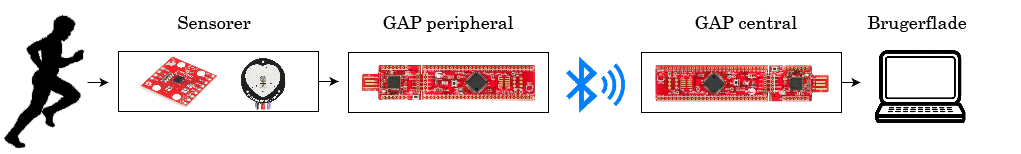
\includegraphics[scale=0.45]{figures/bProblemloesning/blokdiagram.png}
	\caption{På figuren ses blokdiagram for det samlede system, hvor et input modtages fra brugeren gennem sensorer, hvilket behandles i en GAP peripheral MCU. Herefter sendes dataet via BLE til en computer gennem en GAP central MCU, hvor det visualiseres på en brugerflade.}
	\label{fig:design_blokdiagram}
\end{figure}

Blokkene implementeres forskellige stedet i det samlede system, som vist på \figref{fig:design_blokdiagram}, hvoraf spændingsforsyning tilkobles GAP peripheral MCUen, hvor sensorer også tilkobles. På denne MCU vil signalerne blive digitaliseret og algoritmer vil efterfølgende behandle og adskille aktiviteterne gang, løb og cykling, samt udregne en tilhørende puls. Disse data sendes via BLE til en GAP central MCU som er koblet til en computer. På computeren vil dataet blive visualiseret igennem en MATLAB GUI, hvor brugeren kan følge sin progression.\fxnote{Vil vi have denne tekst før eller efter billedet?}  
\section{LSM9DS1}
Der benyttes en IC (LSM9DS1), som både indeholder magnometer, gyroskop og accelerometer. Det er muligt at indstille accelerometeret til $\pm$1, 4, 8 eller 16 g. Gyroskopet kan måle $\pm$245, 500 eller 2000 grader per sekund, og magnometeret kan måle $\pm$4, 8, 12 eller 16 G.\citep{Jimb02016} \newline
LSM9DS1 har ni frihedsgrader, hvormed det måler i x-, y- og z-aksen for både magnometeret, gyroskopet og accelerometeret, hvilket kan ses på \figref{vores_IC}. Akserne for gyroskopet og accelerometeret internt følger højrehåndsreglen, mens magnometerets x- og y-akse er flippet.\citep{Jimb02016}

\begin{figure}[H]
	\centering
	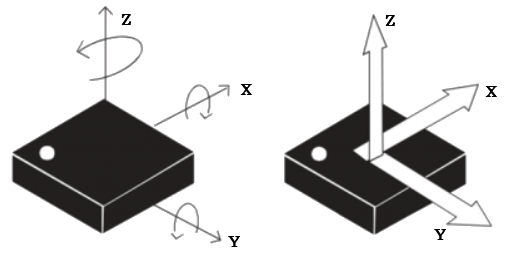
\includegraphics[scale=0.6]{figures/cDesign/LSM9DS1.png}
	\caption{På figuren ses akserne fra IC'en LSM9DS1, hvor magnometerets (til venstre) akse i realiteten er flippet i forhold til gyroskopet (i midten) og accelerometeret (til højre).\citep{Jimb02016}}
	\label{fig:sensor_placering}
\end{figure}

LSM9DS1 er valgt, da den både indeholder et gyroskop og et accelerometer, som der er mulige at benytte enkeltvis eller samlet. Da gyroskopet bruger 4mA og accelerometeret bruger 600$\text muA$, er det væsentligt at kunne sætte gyroskopet i sleepmode, når dette ikke benyttes. 
\section{Pulssensor}
\textit{I dette afsnit beskrives designet, implementeringen og testen af den valgte pulssensor.}

\subsection{Design}
Pulssensoren SEN-11574 er valgt til dette projekt, da det er en optisk pulssensor og er derfor mere sikker for brugeren, som beskrevet i \secref{sec:pulssensor}. Derudover er en optisk pulssensor mere alsidig i forhold til placering, da den blot skal placeres over en arterie. Pulssensoren kræver 3 til 5 V for at være funktionel og forbruger 4 mA ved en forsyning på 5V. På sensorens board findes et aktivt filter\fxnote{Et aktivt filter er en type af analog elektronisk filter, der anvender aktive bestanddele, såsom en forstærker.} samt en forstærker, som tilsammen øger amplituden for pulsbølgen og normaliserer signalet omkring et referencepunkt, hvilket fjerne al DC spænding i signalet. Herved fremkommer en tydelig pulsbølge direkte fra sensoren, som umiddelbart ikke kræver behandling af signalet for at kunne detektere. \citep{Murphy2016,Murphy2016_sensor}

Pulssensoren skal benyttes til at beskrive intensiteten af aktiviteten, som beskrevet i \secref{subsub:ak_int}. Herudfra kan effekten af aktiviteten bestemmes, hvilket kan have en motiverende faktor for brugeren. \\
Sensoren har 3 pins til henholdsvis spændingsforsyning, ground og outputsignal, som skal kobles med MCU'en. Outputsignalets pin skal designes i programmet PSoC Creater, således MCU'en kan finde ud af at modtage signalet fra denne pin. Dette gøres ved at indsætte henholdsvis en UART serie kommunikationsblok (SCB) og SAR ADC i topdesignet. UART'en bruges for at sensoren og MCU'en kan kommunikere og er tilpasset formålet fra standart. Puls data skal igennem en ADC, da det er et analog signal, der fortsætter så længe sensoren modtager en spænding. Dennes design skal derfor tilpasses pulssensoren, hvilket gøres ved at væge antallet af kanaler og samplerate. I dette tilfælde skal der benyttes én kanal, som er single ended, og ADC'ens samplingsfrekvens sættes til 35 SPS. ADC'ens samplingsfrekvens vælges ud fra, at en persons makspuls kan beregnes med 220 - alder \citep{CooperBlair2005}. Ud fra målgruppen vurderes det, at makspulsen altså er cirka 210, som svarer til tre et halvt slag pr sekund. Det vurderes at ti samples per puls giver et præsentabelt resultat, hvilket derved giver 35 SPS.\\
Efter UART og ADC er konfigureret i topdesignet, skal de korrekte pins indstilles i pinopsætning. UART pins får typisk tildelte pins, hvorimod ADC'ens inputpin skal indstilles til den plads, som outputtet fra sensoren er. \\

Igennem et matlab program er det muligt at visualisere pulsen ved hjælp af en GUI. I det samlede system skal denne GUI ikke være tilgængelig her i processen, da GAB peripheral modtager pulsdata og sender dette videre sammen med IC data til GAB central, som skal visualisere data i en endelig GUI.
% Vigtig viden om vores specifikke pulssensor
% Hvordan vi skal bruge den og hvordan dataen herfra skal behandles
% implementering på MCU
\subsection{Test}
% Test af krav


% Grimme hjemmeside \citep{Murphy2016}
% \cite{Murphy2016_sensor}


\begingroup
\raggedright
\bibliographystyle{unsrtnat}
\bibliography{kilder}
\endgroup

\begin{appendices}
	\chapter{Pilotforsøg}\vspace{-.75cm}\label{pilot}
\section{Formål}
Pilotforsøget udføres med henblik på at kunne lave algoritmer ud fra målinger med et accelerometer og gyroskop, som adskiller de tre forskellige aktivitetsformer gang, løb og cykling. Det undersøges derudover hvilke af accelerometerets akser der er essentielle at lave algoritmer ud fra. Ydermere undersøges signalernes frekvens for at undgå aliasing i det endelige system og for at kende nyquistfrekvensen. Sidst undersøges hvilken indflydelse placering af sensoren har på signalets udformning. Dette gøres så det endelige systems signal ikke går i mætning på grund af for stor kraftpåvirkning, og for at undersøge om placering har indflydelse på signalernes udformning.

Til opsamling af data, anvendes en Shimmer 3. Dette er en enhed, som indeholder en række sensorer\fxnote{accelerometer, gyroskop, tryksensor, magnometer, højdemåler}, hvor der til forsøget udelukkende benyttes et accelerometer og et gyroskop. 


%Resultaterne fra pilotforsøget bruges til at designe det endelige system, hvor softwaren for CY8CKIT-043 PSoC 4 M-Series Prototyping Kit skal konfigureres og tilpasses.

Formålet med pilotforsøget er dermed:\vspace{-3mm}
\begin{itemize}
	\item At undersøge hvordan signalerne for gang, løb og cykling adskilles fra hinanden. 
	\item At undersøge hvilken betydning placering af sensorene har for signalets udformning ved de tre aktivitetsformer gang, løb og cykling. 
	\item At bestemme frekvensområdet for signalerne.
	\item At bestemme amplitude for signalerne 
\end{itemize}
%er det nødvendigt at kende signalets frekvensindhold og vide, hvordan forskellige aktivitetsformer påvirker systemet. Målingerne skal undersøges for at kunne lave en algoritme, som kan få sensoren til at skelne imellem de pågældende aktivitetsformer. Derudover skal det bestemmes, hvor sensoren skal placeres på kroppen for mest optimalt udbytte. Derfor er formålet med pilotforsøget følgende:
%\begin{itemize}
%	\item Bestemme hvordan sensoren påvirkes af gang, løb og cykling. (Undersøge signalets udformning for accelerometer og gyroskop ved aktiviteterne; løb, gang og cykling. 
%		- Ligeledes at undersøge placeringen af sensoren ift. påvirkning af signalet.	
%	\item Undersøge hvor mange g-kræfter sensorens målinger ændrer sig alt efter placering på kroppen.
%	\item Undersøge bevægelsesmønstret i signalet i forhold til placering af sensor.
%	\item Bestemme frekvensindholdet for signalet.
%\end{itemize}

\section{Metode}
%Forsøgets metode er bestemt og udført med henblik på at opfylde pilotforsøgets formål. Dette involverer henholdsvis de materialer der skal benyttes samt den fremgangsmåde som ligger til grund for udførelsen.

Til forsøget medtages kun forsøgspersoner, som ikke lider af gener der forhindrer dem i at udføre aktiviteterne gang, løb og cykling. Er en person skadet eller syg, eksluderes denne dermed fra forsøget. Der udføres kun forsøg på gruppemedlemmer, og det er derfor ikke muligt at udføre forsøget på en person fra målgruppen, som er på 8-12 år. Resultaterne kan dermed variere i forhold til målgruppen, da disses vægt og højde vil varierer fra forsøgspersonerne. 

%Forsøget inkluderer udelukkende fuldt funktionsdygtige personer, hvormed ingen forsøgspersoner må have fysiske gener som kan medføre besvær ved udførsel af aktiviterne; gang, løb og cykling. Dermed sikres det, at forsøgets data indeholder normaliserede data som giver grundlag for et validt og repræsentativt datasæt for fysisk funktionsdygtige personer. 

Forsøget vil tage udgangspunkt i tre forudbestemte placeringer på underbenet af enheden, Shimmer3, hvilke kan ses på \figref{fig:sensor_placering}. Disse placeringer er udvalgt på baggrund af \secref{bevaegelse}, hvor det ses at de største bevægelser optræder her i forbindelse med gang, løb og cykling. Accelerometeret registrerer position og acceleration, og det forventes derfor at den største forskel vil kunne ses ved disse placeringer, da det især er distalt for patella, der bevæges under gang og løb. I databehandlingen behandles kun data fra accelerometerets y-akse, da denne på baggrund af \secref{bevaegelse} bør have den største kraftpåvirkning.

%Det er kun placering B der påvirkes af z-aksen ved aktiviteten gang\citep{sabas kilde}, hvormed det formodes at samme påvirkning gælder for løb\citep{RueterboriesSpaichLarsenEtAl2010}. Ud fra bevægelsesanalysen i \secref{bevaegelse}, udledes det ligeledes at alle tre aktiviteter primært er i disse to retninger. 
% Dette vælges på baggrund af bevægelsesanalysen, hvor det blev udledt at den primære bevægelse af  benet ved de tre aktivitetsformer gang, løb og cykling i x- og y-aksens retning \citep{kilde}. \fxnote{måske noget om gyroskop + er det rigtigt i forhold til bevægelsesanalysen??}


% med henhold til æstetiske og brugervenlige aspekter samt \secref{TEORI SENSORER}. \newline
%\textit{Jeg ved ikke helt hvad jeg skal skrive vores begrundelse er ift. det teori om gyroskop, derfor skal de sidste linjer her skrives på senere. Ellers hvis en af jer ved nok om gyroskop til at skrive begrundelsen ;-)}


\subsection{Materialer}
\begin{itemize}
	\item Løbebånd med justerbar hastighed og sikkerhedsbæresele.
	\item Motionscykel.
	\item Shimmer3 sensor med tilhørende holder og strap.
	\item Sportstape.
	\item Computer med følgende software:
	\begin{itemize}
		\item Labview.
		\item Shimmer sensing.
	\end{itemize}
\end{itemize}

\subsection{Fremgangsmåde}
Forsøgets fremgangsmåde er opdelt i to dele. Første del indeholder en opsætning af Shimmer3, mens den anden del er fremgangsmåden for optagelse af data fra forsøget.

\subsubsection{Opsætning af Shimmer3 SUB}
Før forsøgene kan udføres skal Shimmer forbindes korrekt med computeren, og indstilles til at bruge de sensorer der ønskes i pilotforsøget. \vspace{-3mm}
\begin{itemize}
	\item Shimmer forbindes til programmet Labview gennem bluetooth.
	\item Shimmer indeholder en række sensorer, hvoraf følgende skal aktiveres: 
	\begin{itemize}
		\item Widerange Accelerometer.
		\item Gyroscope.
	\end{itemize}
	\item De maksimale arbejdsområder på $\pm$16 g og $\pm$2000 dps vælges, da signalets amplitude endnu er ukendt.
	\item Samplingsfrekvensen indstilles på 512 Hz, da signalets frekvens er ukendt, og denne samplingsfrekvens er den maksimale der kan vælges, når både gyroskopet og accelerometeret er i brug.  
	\item Det er nu muligt at starte stream, og derefter realtime.
	
	
\end{itemize}



%Shimmer3 undersøges nu for at kunne konkludere hvorvidt værdierne fra sensorerne er korrekte. Til denne undersøgelse skal akserne for accelerometeret og gyoskopet findes ved opslag i datablad for enheden. Når disse akser er bestemt, benyttes Labview til at optage målinger i. Der startes en ’Stream’ for at undersøge realtime målingerne.
%Først undersøges accelerometerets værdier ved at placere Shimmer3 på en flad, fast overflade. Shimmer3 vendes i 6 forskellige positioner afhængigt af om det er den positive eller negative akse for x, y eller z som undersøges. Værdien for den positive akse for henholdsvis x, y og z skal vise cirka 9,8 m/s, og med negativt fortegn ved den negative akse for x, y og x. I tilfælde af at værdierne er cirka 9,8 m/s, da kan accelerometerets nøjagtighed godtages. Ydermere undersøges gyroskopet ved at spinne Shimmer3 rundt i en række forskellige retninger for at undersøge hvorvidt sensoren reagerer på dette. Hvis gyroskopet registrerer ændringerne, da godtages dennes nøjagtighed. 
%Shimmer3 er forbundet, konfigureret og undersøgt således forsøget efterfølgende kan gennemføres.

\subsubsection{Udførsel af forsøget}
Forsøget udføres på fire forsøgspersoner, som alle skal udføre aktiviteterne gang, løb, hastigheds stigning og cykling. Den nedenstående beskrivelse af forsøgets fremgangsmåde er gældende for én af de forudbestemte placeringer af Shimmer3 på forsøgspersonens højre ben. Alle fire aktiviteter udføres før placeringen ændres, dog benyttes den samme fremgangsmåde til de resterende to placeringer. De tre placeringer kan ses på \figref{fig:sensor_placering}.

\begin{figure}[H]
	\centering
	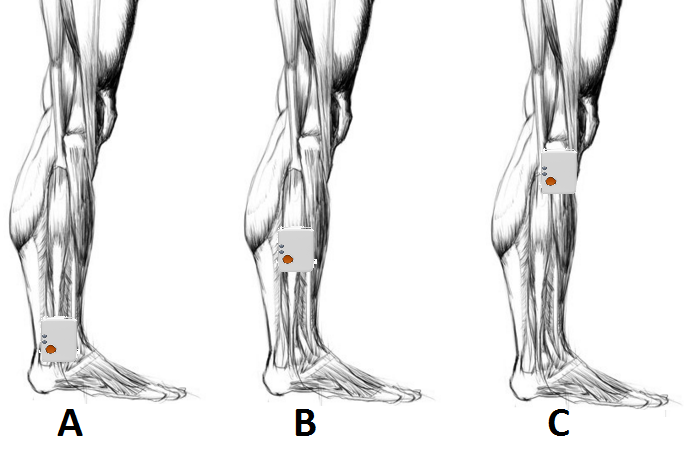
\includegraphics[scale=0.6]{figures/qBilag/Sensor_placering2.png}
	\caption{På figuren ses, hvor sensoren skal placeres under pilotforsøget. Placering A: proximalt for den laterale malleolus. Placering B: medialt på den laterale side af tibia. Placering C: distalt for patella på den laterale side. (Modificeret fra \cite{Perna2016,Shimmer2016})}
	\label{fig:sensor_placering}
\end{figure}

Inden forsøget skal forsøgspersonen fastspændes i en sikkerhedssele, så der ikke opstår skader hvis personen snubler på løbebåndet. Derudover skal forsøgspersonen inden hver måling fortælle hvor på borgskalaen denne befinder sig, og er det under 11 kan målingen påbegyndes. Borgskalaen kan ses på \figref{fig:borgskala}. Denne værdi er valgt for at forsøgspersonen ikke allerede har det som om kroppen er i gang med træning Det sikres dermed at alle forsøgspersoner har samme startbetingelser for alle forsøg. Borgskalaen der benyttes til pilotforsøget kan ses på \figref{fig:borgskala}. 

\begin{figure}[H]
	\centering
	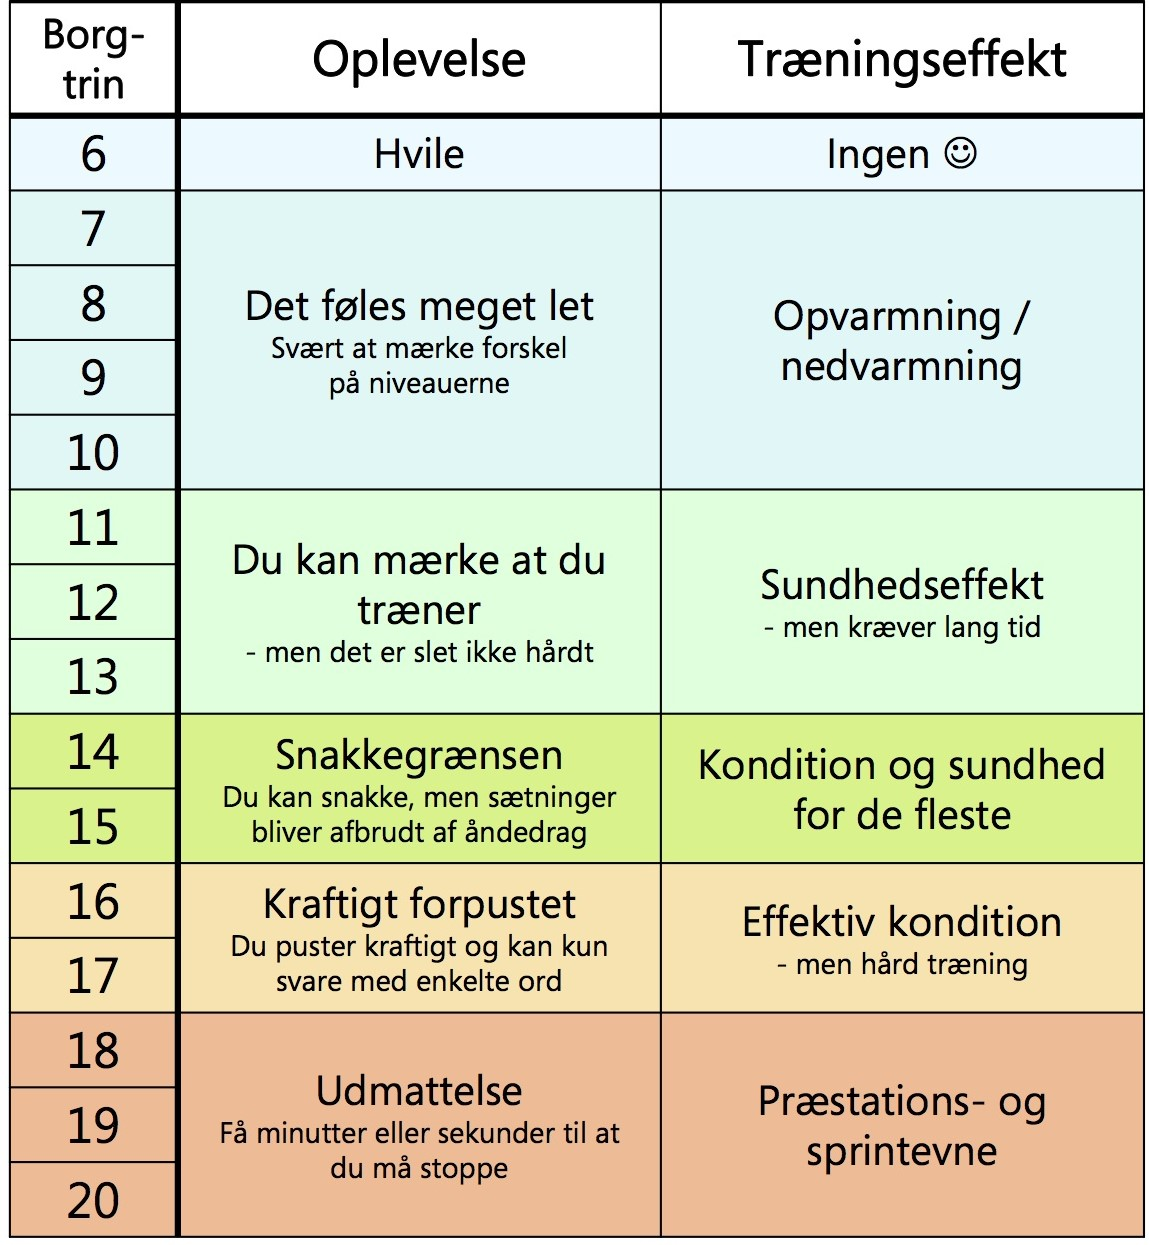
\includegraphics[scale=0.5]{figures/qBilag/Borg-skala.jpg}
	\caption{På figuren ses borgskalaen, som er den der benyttes inden forsøgsstarten. (Modificeret)\cite{Patientinformationen2013})}
	\label{fig:borgskala}
\end{figure}

Første måling er gang, hvor et gangtempo på 4,8 km/t er valgt\citep{Miles2007}. \vspace{-3mm}
\begin{itemize}
	\item Der foretages en baseline på 10 sekunder, hvor forsøgspersonen skal stå oprejst med ret ryg og fødderne placeret parallelt og kigge ligefrem ved baseline målingen.
	\item Løbebåndet indstilles til 4,8 km/t, hvor forsøgspersonen går på løbebåndet indtil en konstant hastighed på løbebåndet opnås. 
	%		\item Forsøgspersonen indikerer når denne føler en homogen bevægelses-cyklus.
	\item Målingen på 45 sekunder igangsættes.
\end{itemize}

Anden måling er løb, et løbetempo på 11,3 km/t er valgt\citep{Miles2007}. \vspace{-3mm}
\begin{itemize}
	\item Der foretages en baseline på 10 sekunder, hvor forsøgspersonen skal stå oprejst med ret ryg og fødderne placeret parallelt og kigge ligefrem ved baseline målingen.
	\item Løbebåndet indstilles til 11,3 km/t, hvor forsøgspersonen løber på løbebåndet indtil en konstant hastighed på løbebåndet opnås. 
	%	\item Forsøgspersonen indikerer når denne føler en homogen bevægelses-cyklus.
	\item Målingen på 45 sekunder igangsættes.
\end{itemize}

Tredje måling foretages på løbebåndet, hvor forsøgspersonen gradvist skal stige i tempo under hele forsøget. Der noteres under forsøget hvornår forsøgspersonen skifter fra gang til løb.  \vspace{-3mm}
\begin{itemize}
	\item Der foretages en baseline på 10 sekunder, hvor forsøgspersonen skal stå oprejst med ret ryg og fødderne placeret parallelt og kigge ligefrem ved baseline målingen.
	\item Målingen igangsættes.
	\item Løbebåndet indstilles til 2 km/t, hvor forsøgspersonen skal gå i 20 sekunder.  
	\item Hastigheden stiger herefter med 2 km/t for hvert 20. sekund, indtil forsøgspersonen har opnået maksimal hastighed, eller løbebåndets maksimale hastighed på 18 km/t. 
	\item Målingen stoppes. 
\end{itemize}

Sidste måling er cykling, hvor et cykeltempo på 20,9 km/t er valgt, hvilket er et højt cykeltempo\citep{Miles2007}. Tempoet er dog underordnet, da der kun ønskes at se på forskellen i selve bevægelsen fra de andre aktivitetsformer, men der er valgt et fast tempo for at få et ensformigt signal. \vspace{-3mm}
\begin{itemize}
	\item Der foretages en baseline på 10 sekunder, hvor forsøgspersonen skal sidde i en naturlig cykelposition på motionscyklen med begge fødder på pedalerne, hvoraf den højre pedal skal være helt i bund. Denne position er valgt, da den er mulig at lave tilnærmelsesvis ens for alle forsøgspersoner, hvormed de får den samme baseline.
	\item Forsøgspersonen træder i pedalerne indtil denne opnår en konstant hastighed på 20,9 km/t ved en belastning på 35 W. Dermed sikres det at alle forsøgspersoner bruger den samme belastning gennem forsøget.  
	\item Målingen på 45 sekunder igangsættes. 
\end{itemize}

Efter de tre placeringer skulle forsøgspersonerne vurdere hvilken placering der var mest behagelig.

\section{Databehandling}
\subsection{Kalibrering af Shimmer}
Forud for pilotforsøgets målinger blev Shimmer kalibreret og testet. For at undersøge hvorvidt kalibreringen af Shimmer fungerede optimalt, blev der opsamlet data til at be-, eller afkræfte dette. Data fra de tre akser, x, y og z blev behandlet. \\
Når Shimmer er placeret i en kalibreringsboks på et bord med henblik på en respektiv akse, bør accelerometeret blive påvirket med $\pm$1 g, mens de resterende akser ikke bør påvirkes.

\begin{figure}[H]
	\centering
	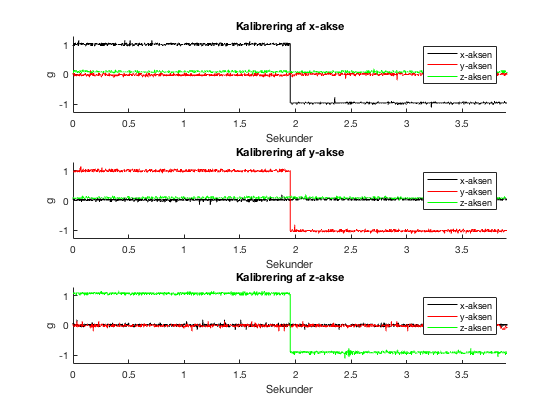
\includegraphics[scale=0.68]{figures/qBilag/kalibreringsdata}
	\caption{På figuren ses kalibreringsdataene tilhørende accelerometerets x, y og z-akse.}
	\label{fig:Ap_Kalibrering}
\end{figure}

For hver akse blev den gennemsnitlige værdi, for henholdsvis den positive- og negative akse, beregnet og sammenholdt med $\pm 1$g. Dermed blev den procentmæssige afvigelse fra tyngdeaccelerationen fundet. Dette resulterede i at x-aksen gennemsnitlig afveg henholdsvis 3,5\% i den negative akse og -2,2\% i den positive akse. Y-aksen afveg gennemsnitligt -2,6\% i den negative akse og -0,6\% i den positive akse. Z-aksen afveg  gennemsnitligt med 8,8\% i den negative akse og 8,0\% i den positive akse. \newline
Kalibreringen blev foretaget for at sikre at et offset ikke var til stede. 

\subsection{Baseline af gang, løb og cykling}
Forud for hver enkelt måling blev der foretaget en baselinemåling som indikation for hvorvidt Shimmer fungerede forud for aktiviteten. Derudover blev det ud fra baseline testet hvorvidt shimmer var i samme position for alle forsøgspersoner ved de forskellige målingers start. Dataene skal afspejle en tilnærmelsesvis fuldstændig tyngdekraftpåvirkning på accelerometerets y-akse, som resultat af Shimmers placering på benet. Baseline blev foretaget for at sikre at shimmer tilnærmelsesvis blev placeret ens på alle forsøgspersoner, hvormed data kunne sammenholdes. 

\begin{table}[H]
	\centering
	\begin{tabular}{cccc}
		\hline
		\rowcolor[HTML]{C0C0C0} 
		{\color[HTML]{333333} Forsøgsperson} & {\color[HTML]{333333} \begin{tabular}[c]{@{}c@{}}Placering A, \\ y-akse {[}g{]}\end{tabular}} & {\color[HTML]{333333} \begin{tabular}[c]{@{}c@{}}Placering B,\\ y-akse {[}g{]}\end{tabular}} & {\color[HTML]{333333} \begin{tabular}[c]{@{}c@{}}Placering C,\\ y-akse {[}g{]}\end{tabular}} \\ \hline
		F1 & 0,98 & 0,99 & 0,97 \\ \hline
		F2 & 1 & 0,99 & 0,96 \\ \hline
		F3 & 0,98 & 0,98 & 0,98 \\ \hline
		F4 & 0,97 & 0,99 & 0,95 \\ \hline
	\end{tabular}
	\caption{I tabellen ses de gennemsnitlige baselineresultater fra accelerometerets y-akse forud for gang.}
	\label{fig:Ap_baselinegang}
\end{table}\vspace{-0.5cm}

\begin{table}[H]
	\centering
	\begin{tabular}{cccc}
		\hline
		\rowcolor[HTML]{C0C0C0} 
		{\color[HTML]{333333} Forsøgsperson} & {\color[HTML]{333333} \begin{tabular}[c]{@{}c@{}}Placering A, \\ y-akse {[}g{]}\end{tabular}} & {\color[HTML]{333333} \begin{tabular}[c]{@{}c@{}}Placering B,\\ y-akse {[}g{]}\end{tabular}} & {\color[HTML]{333333} \begin{tabular}[c]{@{}c@{}}Placering C,\\ y-akse {[}g{]}\end{tabular}} \\ \hline
		F1 & 0,99 & 0,99 & 0,97 \\ \hline
		F2 & 0,99 & 0,99 & 0,96 \\ \hline
		F3 & 0,97 & 0,98 & 0,98 \\ \hline
		F4 & 0,97 & 0,99 & 0,95 \\ \hline
	\end{tabular}
	\caption{I tabellen ses de gennemsnitlige baselineresultater fra accelerometerets y-akse forud for løb.}
	\label{fig:Ap_baselineloeb}
\end{table}\vspace{-0.5cm}

Ved cykling benyttes gyroskopets data, da cykling detekteres som en roterende bevægelse omkring z-aksen. Enheden af dataet heraf er grader per sekund (dps), og dermed bør baselineresultaterne ligge omkring nul.
\begin{table}[H]
	\centering
	\begin{tabular}{cccc}
		\hline
		\rowcolor[HTML]{C0C0C0} 
		{\color[HTML]{333333} Forsøgsperson} & {\color[HTML]{333333} \begin{tabular}[c]{@{}c@{}}Placering A, \\ z-akse {[}dps{]}\end{tabular}} & {\color[HTML]{333333} \begin{tabular}[c]{@{}c@{}}Placering B,\\ z-akse {[}dps{]}\end{tabular}} & {\color[HTML]{333333} \begin{tabular}[c]{@{}c@{}}Placering C,\\ z-akse {[}dps{]}\end{tabular}} \\ \hline
		F1 & -0,98 & -0,83 & -0,87 \\ \hline
		F2 & -0,90 & -0,79 & -0,77 \\ \hline
		F3 & -0,68 & -0,58 & -0,99 \\ \hline
		F4 & -0,89 & -0,92 & -0,85 \\ \hline
	\end{tabular}
	\caption{I tabellen ses de gennemsnitlige baselineresultater fra gyroskopets z-akse forud for cykling.}
	\label{fig:Ap_baselinecykling}
\end{table}\vspace{-0.5cm}

\subsection{Minimum og maksimum g-påvirkning under gang, løb og hastighed}
Dataene fra aktiviteterne, gang, løb og hastigheds stigning blev alle behandlet med henblik på bestemmelse af den maksimale g påvirkning heraf. Dette blev bestemt af den maksimale påvirkning i henholdsvis accelerometerets positive og negative y-akse samt placeringer. Før forsøgene blev baseline målt inden hvert forsøg. 

Den største afvigelse fra tyngdeaccelerationen for gang var på 0.9969\%, hvormed der vurderes at alle baselines har ligget neutralt. \newline
Nedstående tabel viser resultaterne fra gang med et tempo på 4,8 km/t.
\begin{table}[H]
	\centering
	\begin{tabular}{cccc}
		\hline
		\rowcolor[HTML]{C0C0C0} 
		Forsøgsperson & \begin{tabular}[c]{@{}c@{}} Placering A {[}g{]}\end{tabular} & \begin{tabular}[c]{@{}c@{}} Placering B {[}g{]}\end{tabular} & \begin{tabular}[c]{@{}c@{}} Placering C {[}g{]}\end{tabular} \\ \hline
		F1 &  0,09 ; 2,51  & 0,00 ; 2,32  & -2,51 ; 3,33 \\ \hline
		F2 &  -0,19 ; 3,19 & -0,43 ; 3,04 & -0,97 ; 2,84 \\ \hline
		F3 &  -0,24 ; 3,52 & -0,39 ; 3,38 & -0,20 ; 2,51 \\ \hline
		F4 &  -0,04 ; 2,84 & -0,29 ; 3,62 & -0,50 ; 3,52 \\ \hline
	\end{tabular}%
	\caption{I tabellen ses de maksimale positive og negative værdier fra accelerometerets y-akse som resultat af gang med en hastighed på 4,8 km/t. Værdierne er fundet for både placering A, B og C.}
	\label{fig:Ap_maxggang}
\end{table}

Det ses dermed at den maksimale påvirkning i positiv retning af accelerometerts y-akse under gang ved 4,8 km/t var 3,015 Hz $\pm$0,505 for placering A, 3,095 Hz $\pm$0,53 for placering B og 3,05 Hz $\pm$0,47 for placering C.\newline
Den maksimale påvirkning i negativ retning af accelerometerets y-akse under gang ved 4,8 km/t var 0,018 Hz $\pm$0,88 for placering A, -0,28 Hz $\pm$0,28 for placering B og -1,05 Hz $\pm$0,85 for placering C. 

På samme måde blev baseline fundet for løb ved en hastighed på 11,3 km/t, som maksimalt afveg med 0,9930\%. Det vurderes derfor at baseline for alle forsøgspersoner inden løb ligger neutralt. Herefter blev der fundet de maksimale positive og negative værdier for løb, som kan ses i nedstående tabel.  
\begin{table}[H]
	\centering
	\begin{tabular}{cccc}
		\hline
		\rowcolor[HTML]{C0C0C0} 
		Forsøgsperson & \begin{tabular}[c]{@{}c@{}} Placering A {[}g{]}\end{tabular} & \begin{tabular}[c]{@{}c@{}} Placering B {[}g{]}\end{tabular} & \begin{tabular}[c]{@{}c@{}} Placering C {[}g{]}\end{tabular} \\ \hline
		F1 &  -2,03 ; 8,59 & -2,80 ; 5,07 & -4,10 ; 3,33 \\ \hline
		F2 &  -0,97 ; 5,35 & -2,51 ; 6,13 & -4,44 ; 6,52 \\ \hline
		F3 &  -2,12 ; 5,55 & -1,83 ; 5,60 & -2,46 ; 5,60 \\ \hline
		F4 &  -3,48 ; 6,42 & -4,63 ; 6,76 & -3,52 ; 8,30 \\ \hline
	\end{tabular}%
	\caption{I tabellen ses de maksimale positive og negative værdier fra accelerometerets y-akse som resultat af løb med en hastighed på 11,3 km/t. Værdierne er fundet for både placering A, B og C.
	}
	\label{fig:Ap_maxgloeb}
\end{table}
Det ses dermed at den maksimale påvirkning i positiv retning af accelerometerets y-akse under gang ved 11,3 km/t var 6,48 Hz $\pm$2,11 for placering A, 5,89 Hz $\pm$0,87 for placering B og 5,94 Hz $\pm$2,36 for placering C.\newline
Den maksimale påvirkning i negativ retning af accelerometerets y-akse under gang ved 11,3 km/t var -2,15 Hz $\pm$1,18 for placering A, -2,94 Hz $\pm$1,11 for placering B og -3,63 Hz $\pm$1,17 for placering C. 

Slutvis blev accelerometerets y-akse undersøgt ved forsøget hvor forsøgspersonerne gradvist steg i tempo. Baseline for disse målinger afveg med 0,9954\% hvormed det vurderes at baseline for alle målinger var neutrale. Den maksimale påvirkning i henholdsvis positiv og negativ retning der blev detekteret under hastighedsstigningen kan ses i nedstående tabel. 
\textit{Hastigheds stigning:}
\begin{table}[H]
	\centering
	\begin{tabular}{cccc}
		\hline
		\rowcolor[HTML]{C0C0C0} 
		Forsøgsperson & \begin{tabular}[c]{@{}c@{}} Placering A {[}g{]}\end{tabular} & \begin{tabular}[c]{@{}c@{}} Placering B {[}g{]}\end{tabular} & \begin{tabular}[c]{@{}c@{}} Placering C {[}g{]}\end{tabular} \\ \hline
		F1 &  -3,04 ; 8,20  & -4.59 ; 6,28  & -6,66 ; 7,10 \\ \hline
		F2 &  -3,19 ; 10,96 & -4,49 ; 10,48 & -7,58  ; 9,61 \\ \hline
		F3 &  -4,92 ; 10,48 & -4,59 ; 13,13 & -4,63 ; 9,70 \\ \hline
		F4 &  -8,83 ; 16,95 & -7,48 ; 16,32 & -8,01 ; 15,35 \\ \hline
	\end{tabular}%
	\caption{I tabellen ses de maksimale positive og negative værdier fra accelerometerets y-akse som resultat af hastigheds stigning. Værdierne er fundet for både placering A, B og C.}
	\label{fig:Ap_maxghastighed}
\end{table}
Det ses dermed at den maksimale værdi målt i påsitiv etning på accelerometerets y-akse under hastighedsstigningen var 11,65 Hz $\pm$5,3 ved placering A, 11,55 Hz $\pm$4,77 for placering B og 10,44 Hz $\pm$4,91 for placerinng C. \newline
Den maksimale påvirkning i negativ retning for accelerometerets y-akse under hastighedsstigningen var -5,00 Hz $\pm$1,96 for placering A, -5,29 Hz $\pm$0,8 for placering B og -6,72 Hz $\pm$2,09 for placering C.\newline


\subsection{Maksimal omdrejninger per sekund under cykling}
Dataene fra aktiviteten, cykling, blev behandlet med henblik på bestemmelse af den maksimale amplitude fra gyroskopet. Dette blev bestemt ved at beregne den maksimale peak-to-peak, under udførelsen af cykling. Dataene blev kun behandlet med henblik på gyroskopets z-akse, som resultat af \secref{bevaegelse}. Inden dataopsamling for cykling, blev der målt en baseline. Den maksimale afvigelse fra nul var -0,9979\%, hvormed det vurderes at alle målinger havde en neutral baseline. Dataene fra forsøget kan ses i nedstående tabel.


\begin{table}[H]
	\centering
	\resizebox{\textwidth}{!}{%
		\begin{tabular}{cccc}
			\hline
			\rowcolor[HTML]{C0C0C0} 
			Forsøgsperson & \begin{tabular}[c]{@{}c@{}} Placering A {[}g{]}\end{tabular} & \begin{tabular}[c]{@{}c@{}} Placering B {[}g{]}\end{tabular} & \begin{tabular}[c]{@{}c@{}} Placering C {[}g{]}\end{tabular} \\ \hline
			F1 & -148,23 ; 108,29   & -209,82 ; 118,60   & -188,66 ; 98,29  \\ \hline
			F2 & -108,42 ; 108,11   & -133,11 ; 114,94	 & -150,43 ; 120,61 \\ \hline
			F3 & -208,29 ; 136,28  	& -196,95 ; 140,18	 & -195,43 ; 151,10 \\ \hline
			F4 & -182,56 ; 152,13  	& -159,82 ; 138,35	 & -152,62 ; 136,83 \\ \hline
		\end{tabular}%
	}
	\caption{I tabellen ses de maksimale positive og negative værdier fra gyroskopets z-akse som resultat af cykling med en hastighed på 20,9 km/t. Værdierne er fundet for både placering A, B og C.}
	\label{fig:Ap_maxghastighed}
\end{table}
Det ses dermed at den maksimale påvirkning i positiv retning af gyroskopet under cykling ved en hastighed på 20,9 km/t var 126,20 dps $\pm$25,93 for placering A, 128,02 dps $\pm$12,16 for placering B og 126,71 dps $\pm$24,39 for placering C. 
Den maksimale påvirkning i negativ retning er -161,88 dps $\pm$53,46 for placering A, -174,93 dps $\pm$41,82 for placering B og -171,79 dps $\pm$21,36 for placering C. 

\subsection{Afgrænsning af placering}
Databehandling vil ud fra de maksimale værdier tage udgangspunkt i placering A. Dette gøres på baggrund af at denne er den mest optimale placering i forhold til komfort for brugeren, da tre ud af fire forsøgspersoner foretrak denne placering. Den maksimale værdi for placering A overskrider den maksimale accelerationskraftpåvirkning med 0,95 g. Det vurderes dog at placering A vil være optimal at bruge da de 16,95 g repræsenteres i form af hælnedslag. Det vil stadig være muligt at adskille hælnedslag fra tåafsæt selvom det vil klippes ved 16 g. \newline
Gyroskopets data viser ligeledes at det er muligt at benytte placering A, da denne viser at cykling ikke resulterer i en høj dps. 
På baggrund af dette vil der i det resterende databehandling tages udgangspunkt i placering A, som kan ses i to sekunders interval for hver af de fire forsøgspersoner på \figref{raa_data}.

\begin{figure}[H]
	\centering
	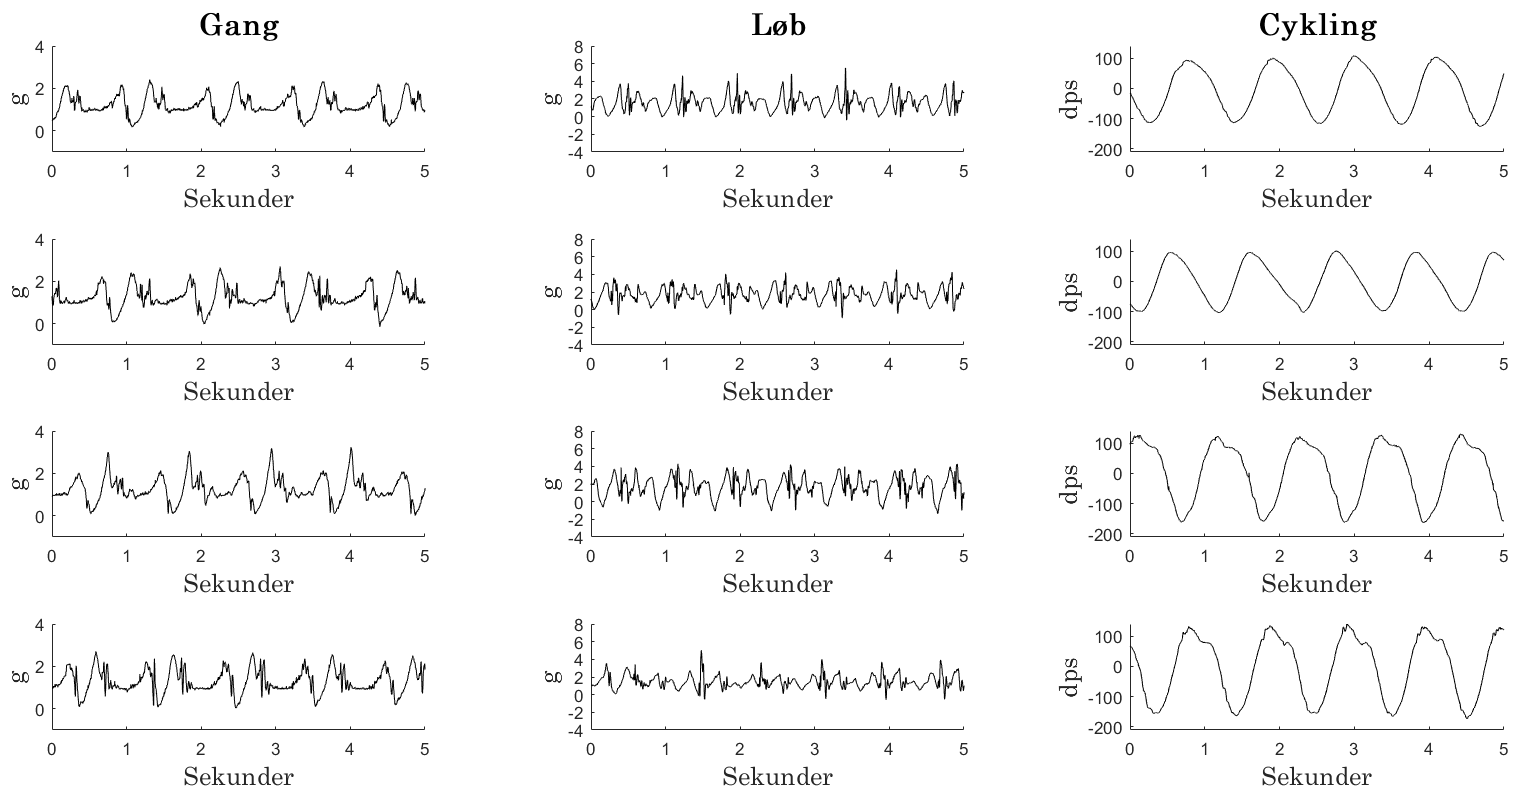
\includegraphics[scale=0.38]{figures/qBilag/raa_data}
	\caption{På figuren ses det ubehandlede data fra de tre aktivitetstyper gang, løb og cykling optaget på henoldsvis et accelerometer og et gyroskop ved placering A.}
	\label{raa_data}
\end{figure}


\subsection{Frekvensindhold af gang, løb og cykling}
Dataene fra aktiviteterne, gang og løb blev behandlet for at bestemme signalernes frekvensindhold. Resultatet af dette muliggør bestemmelsen af samplingsfrekvensen vedrørende accelerometeret og gyroskopet. Der blev foretaget en frekvensdomæne analyse, hvilket muliggør visualisering af signalets magnitude ved forskellige frekvenser, hvoraf energien af signalet kommer til udtryk.

\begin{figure}[H]
	\centering
	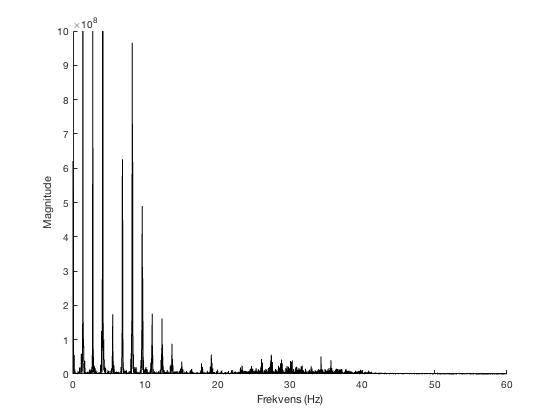
\includegraphics[scale=0.68]{figures/qBilag/fft_f1_loeb}
	\caption{På figuren ses frekvensdomænet af aktiviteten løb for forsøgsperson 1. Den fuldstændige magnitude for de lave frekvenser vises ikke til fulde. Hvis dette skulle være tilfældet ville de mindste magnituder på figuren blive udskalleret.}
	\label{fig:Ap_FFt}
\end{figure}
Frekvensdomæneanalysen vises kun for løb af F1 da frekvensspektrummet var størst heraf. Derudover vises den ikke for gang, da denne ydermere var lavere end for løb, og da begge aktiviteter skal detekteres med et accelerometer, skal de have samme samplingsfrekvens. Dermed vises kun frekvensspektrummet or løb, da systemets samplingsfrekvens bestemmes i forhold til den højest målte frekvens.

Dataene fra aktiviteten, cykling blev behandlet for at bestemme signalernes frekvensindhold, med henblik på bestemmelsen af samplingsfrekvensen vedrørende gyroskopet.
\begin{figure}[H]
	\centering
	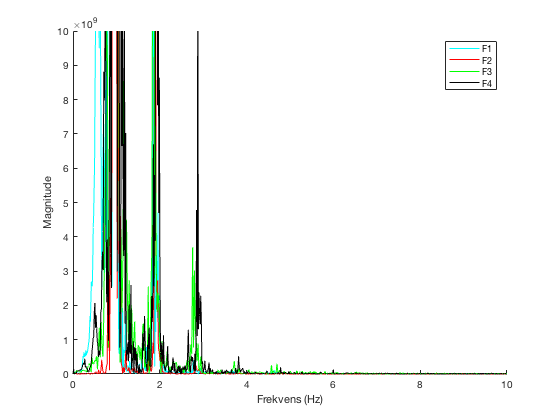
\includegraphics[scale=0.68]{figures/qBilag/cykling_frekvens}
	\caption{På figuren ses frekvensdomænet af aktiviteten cykling for alle forsøgspersoner. Den fuldstændige magnitude for de lave frekvenser vises ikke til fulde. Hvis dette skulle være tilfældet ville de mindste magnituder på figuren blive udskalleret.}
	\label{fig:Ap_cyklingfrekvens}
\end{figure}

\subsection{Accelerometer karakteristika vedrørende gang og løb}
Dataene fra aktiviteten gang og løb blev behandlet med henblik på bestemmelse af signalets karakteristika, således en sammenligning og senere algoritmedesign blev muliggjort. Dataene fra accelerometerets y-akse blev for alle forsøgspersoner lavpas filtreret ved 45 Hz, grundet frekvensspektret på \figref{fig:Ap_FFt}. Derudover vlev signalet differentieret hvormed områderne med størst hældningskoefficient kommer til udtryk. Dermed fremhæves hælnedslag og tåafsæt da disse events har en stor hældning.

\textit{Gang:}
\begin{figure}[H]
	\centering
	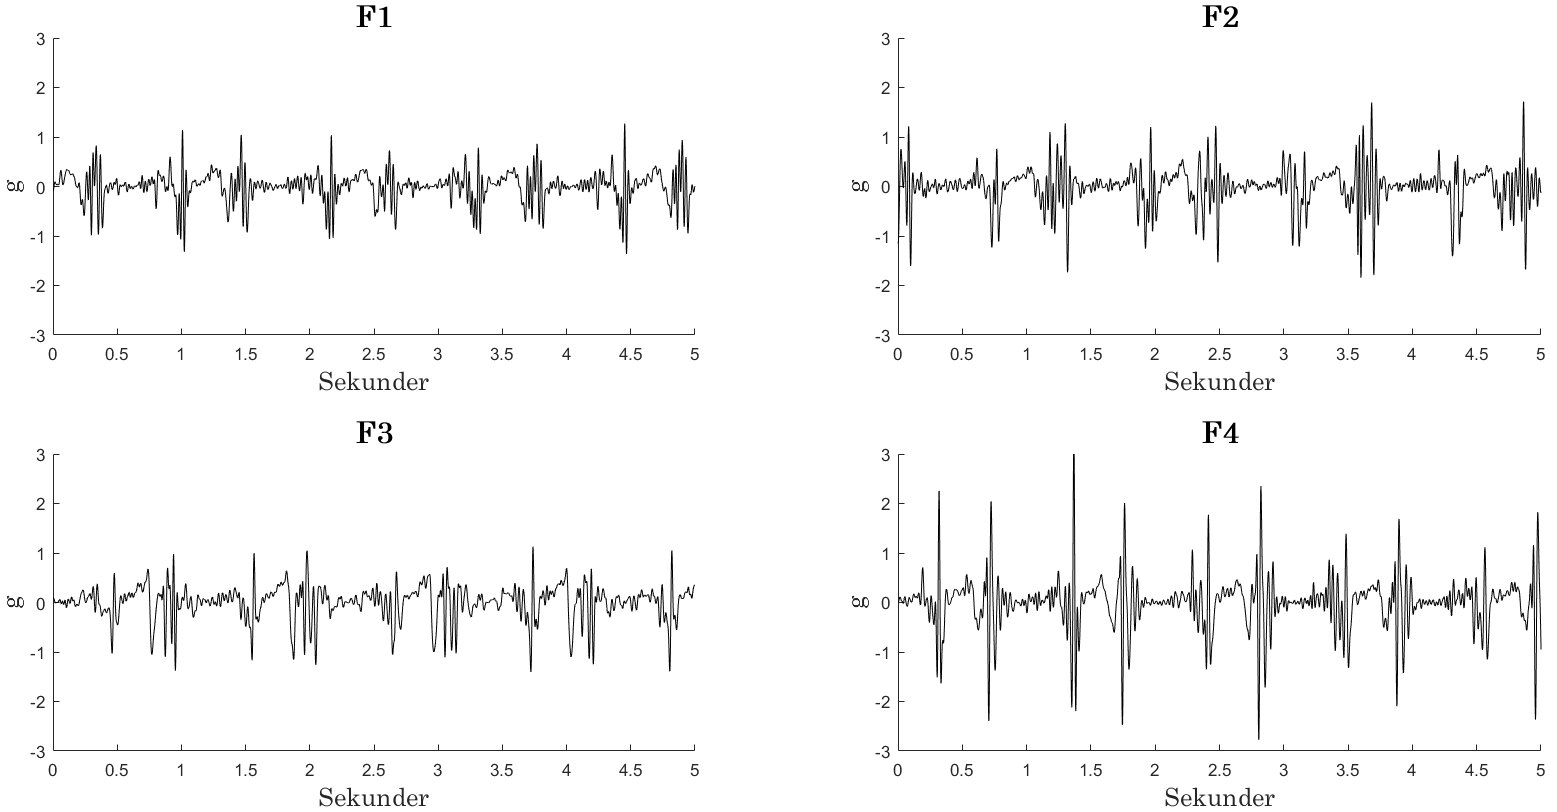
\includegraphics[scale=0.68]{figures/qBilag/gang_diff}
	\caption{På figuren ses det filtrerede og differentierede data fra aktiviteten gang for alle forsøgspersoner.}
	\label{fig:Ap_gangdiff}
\end{figure}

Det ses at hælnedslagg og tåafsæt fremgår tydligere end på \figref{raa_data} for både gang, som kan ses på \figref{fig:Ap_gangdiff} og løb, som kan ses på \figref{fig:Ap_loebdiff}.

\begin{figure}[H]
	\centering
	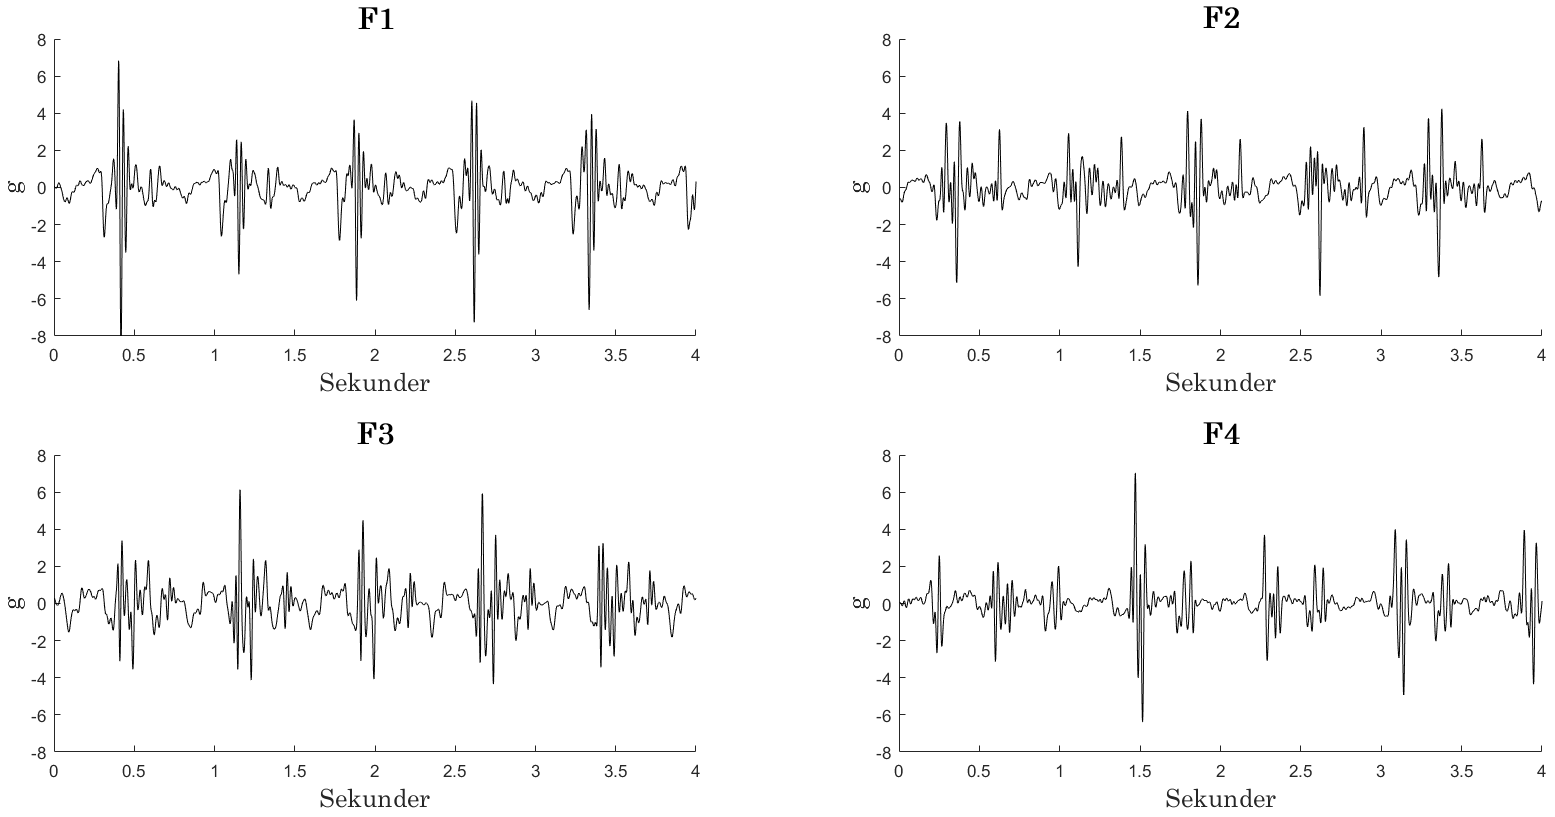
\includegraphics[scale=0.68]{figures/qBilag/loeb_diff}
	\caption{På figuren ses det filtrerede differentierede data fra aktiviteten løb for alle forsøgspersoner.}
	\label{fig:Ap_loebdiff}
\end{figure}

\subsection{Gyroskop karakteristika vedrørende gang, løb og cykling}
Dataene fra aktiviteterne gang, løb og cykling, blev behandlet med henblik på bestemmelse af signalets karakteristika. Dette blev udført ved at sammensætte forsøgspersonernes data, således en sammenligning blev muliggjort. Aktiviteterne gang og løb blev behandlet for at sikre dette ikke havde samme karakteristika som cykling, med henblik på algoritmedesign. Dataene blev kun behandlet med henblik på gyroskopets z-akse, som resultat af \secref{bevaegelse}.  

\textit{Gang:}
\begin{figure}[H]
	\centering
	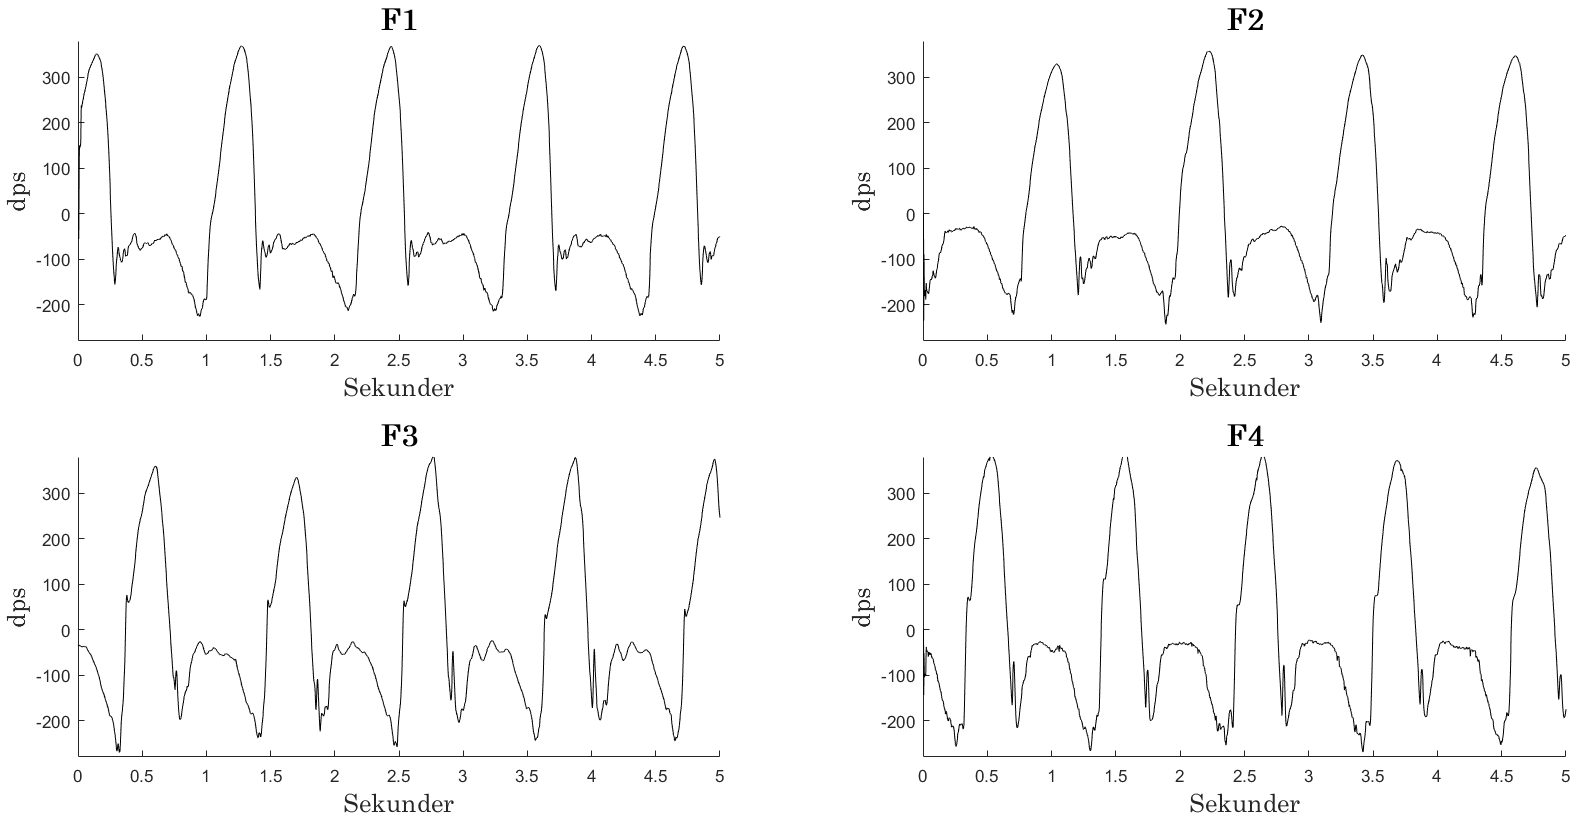
\includegraphics[scale=0.5]{figures/qBilag/gang_gyro}
	\caption{På figuren ses dataene fra gang ved 4,8 km/t fra de fire forsøgspersoner. Dataene er fra gyroskopets z-akse.}
	\label{fig:Ap_cykling}
\end{figure}

\textit{Løb:}
\begin{figure}[H]
	\centering
	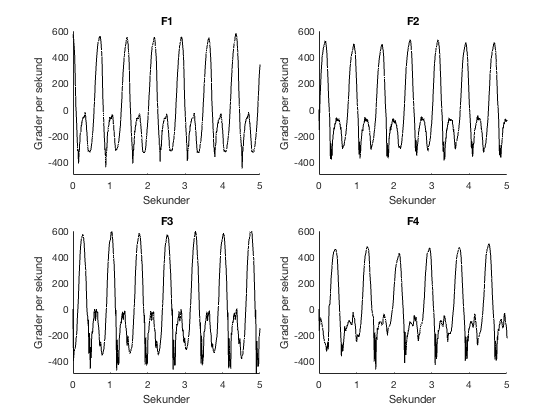
\includegraphics[scale=0.5]{figures/qBilag/loeb_gyro}
	\caption{På figuren ses dataene fra løb ved 11,3 km/t fra de fire forsøgspersoner. Dataene er fra gyroskopets z-akse.}
	\label{fig:Ap_cykling}
\end{figure}

\textit{Cykling:}
\begin{figure}[H]
	\centering
	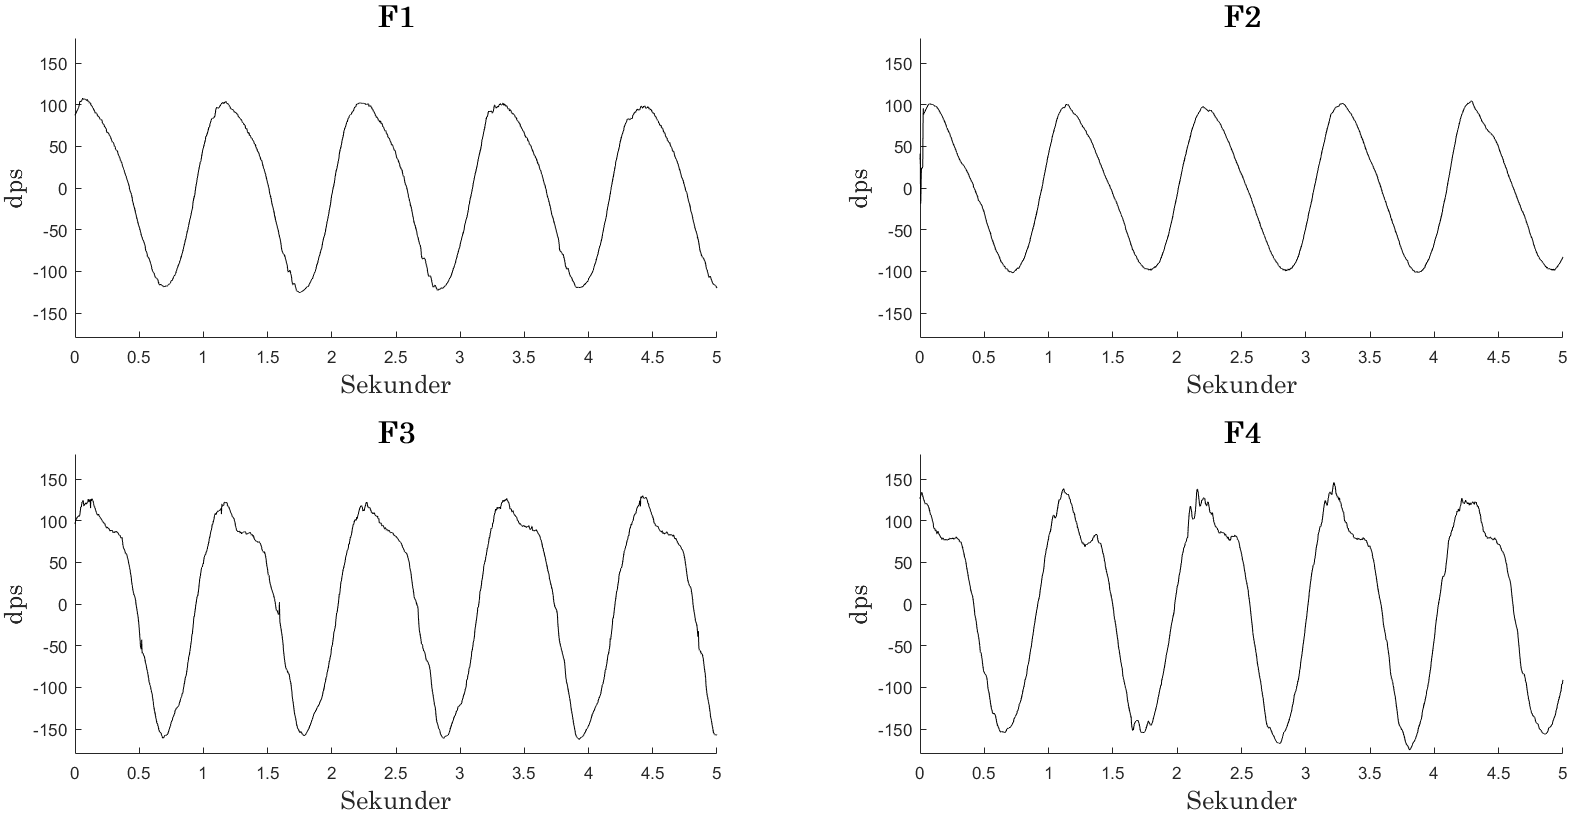
\includegraphics[scale=0.5]{figures/qBilag/cykling_gyro}
	\caption{På figuren ses dataene fra cykling ved 20,9 km/t fra de fire forsøgspersoner. Dataene er fra gyroskopets z-akse.}
	\label{fig:Ap_cykling}
\end{figure}

\section{Diskussion}
\subsection{Kalibrering af Shimmer}
Resultatet af databehandlingen bevirker at kalibreringen af Shimmer antages at være tilstrækkelig. Dette antages at være tilstrækkeligt, da y-aksen  afviger med henholdsvis -2,6\% i den negative akse og -0,6\% i den positive akse, fra den teoretiske værdi. En eventuel fejlkilde til at denne fejlmargin forekom, kunne være at bordet hvorpå Shimmer var placeret, ikke var i vatter.

\subsection{Baseline af gang, løb og cykling}
Baselinemålingerne for henholdsvis gang og løb resulterede i en enslignende påvirkning. Som forventet var g påvirkningen ikke 1 g, hvilket kan være et resultat af at Shimmer ikke er placeret ortogonalt på y-aksen på benet. I og med Shimmer ikke var placeret ortogonalt på benet, kan der være opstået en lille hældning, hvorfor y-aksen ikke påvirkes med præcist 1 g. Resultaterne fra disse målinger indikerer at Shimmer har optaget data som stemmer overens med antagelsen om den tilnærmelsesvise påvirkning på 1 g. 

Resultaterne fra baselinemålingerne vedrørende cykling ligger som forventet omkring nul, hvilket er et resultat af at Shimmer ikke er blevet påvirket i z-aksen i nogen væsentlig grad, da benet ikke bevæges. Resultaterne af disse målinger indikerer at Shimmer har optaget data som stemmer overens med antagelsen om den tilnærmelsesvise påvirkning på 0 dps\fxnote{maksimal afvigelse på -0,9979}. 

\subsection{Maksimal g-påvirkning under gang, løb og hastighed} \label{app:maxg}
Resultatet af databehandlingen vedrørende de tre aktiviteter med henblik på bestemmelsen af den maksimale g påvirkning, medførte at aktiviteten med hastighedsstigning havde den største påvirkning. Resultaterne fra placering A, B eller C fra F1, F2 og F3 ikke overskrider $\pm 16g$. Resultaterne fra F4 overskrider 16 g med 0,95 g. Dette vuredres dog til ikke at have en væsentligt betydning, hvoraf den mest fordelagtige placering vælges. Med baggrund i \secref{succeskrav} og \secref{funktionellekrav} skal placeringen ikke være til gene for barnet, og så skal nemt af-, og påmonteres, hvoraf placering A er valgt, da denne blev valgt som den mest komfortable bland forsøgspersonerne. Dette medfører at den videre resultatbehandling udelukkende tog udgangspunkt i placering A. 

\subsection{Maksimal omdrejninger per sekund under cykling}
Resultatet af databehandlingen vedrørende maksimal omdrejninger ved cykling resulterede i et spænd mellem 216,5 dps og 320,4 dps. Dette kan være et resultat af at forsøgspersonerne ikke har holdt samme hastighed, hvoraf en pludselig acceleration kan betyde en ændring som ikke er relateret til cykling ved 20,9 km/t. I takt med at der maksimalt blev registreret 320,4 dps, er dette medbestemmende vedrørende valg af et endeligt gyroskop. Et gyroskop til det endelige system skal heraf have et arbejdsområde som er større end 320,4 dps, men det præcise arbejdsområde vides ikke, da en hastighedsstigning ikke blev foretaget for cykling.

\subsection{Frekvens indhold af løb og cykling}
Databehandlingen af frekvensindholdet fra gang og løb medførte at det største frekvensspektrum lå mellem 0 og 45Hz. Dette medfører at samplingsfrekvensen vedrørende data fra accelerometeret kan bestemmes. 

Databehandling af frekvensindholdet fra cykling medførte at det største frekvensspektrum lå mellem 0 og 6 Hz. Dette medfører at samplingsfrekvensen vedrørende data fra gyroskopets kan bestemmes. 

\subsection{Accelerometer karakteristika vedrørende gang og løb}
Databehandlingen vedrørende accelerometerets karakteristika af gang og løb resulterede i en sammenligning af dataene. Dataene fra gang viser to events hvor peaks fremstår. Disse har en relativ kort afstand til hinanden, efterfulgt af en længere pause, hvilket flere figurer i \secref{bevaegelse} viser som henholdsvis hælnedslag og tåafsæt. Ligeledes for løb var disse forskellige events, som også antages værende hælnedslag og tåafsæt. Der forekom dog yderligere et harmonisk peak som var betydeligt større end de andre events. Yderligere behandling af aktiviteternes data med anerkendte algoritmer kan være nødvendig, men databehandlingen medførte at gang og løbs karakteristika kan bestemmes og heraf adskilles. Dette er muligt idet varigheden mellem de antagede hælnedslag forekommer $\approx$~0,43 sekunder hurtigere ved løb end ved gang.\fxnote{hvis dette skal med skal er overvejes om man altid kan sige 0,43 sekunder, eller om man skal lave det relativt i forhold til tid (60/40)}

\subsection{Gyroskop karakteristika vedrørende gang, løb og cykling}
Databehandlingen af gyroskopets karakteristika vedrørende gang, løb og cykling resulterede i en sammenligning heraf. Resultatet af dette tyder på, at data fra et gyroskops z-akse tilhørende cykling, tilnærmelsesvis kan afspejles som en sinus-bølge, samt at gang og løb antageligvis ikke kan forveksles heraf. Dette muliggør algoritmedesign med henblik på detektering af cykling. Det kan antages at resultater fra cykling ved forskellige hastigheder vil påvirke signalet i en grad hvor frekvens og amplitude ændres.

\section{Konklusion}
I pilotforsøget blev aktiviteterne gang, løb og cykling undersøgt i en biomekanisk sammenhæng. Ud fra kalibreringen vurderes shimmer til at måle korrekt i de forskellige akser. Derudover vise alle baselines at blive påvirket med mindre end 1\% vigende fra det forventede, hvormed det vurderes at alle data kan sammenlignes, da shimmer tilnærmelsesvis er placeret ens ved alle målinger for alle forsøgspersoner. \newline
Signalerne for gang og løb adskilles ved at de maksimale målte amplituder for løb tilnærmelsesvis er dobbelt så stor, som for gang, men ellers ser signalerne ensformige ud. Cykling målt med et gyroskop adskilles væsentligt fra gang og løb, da cykling ikke har store peaks, men i stedet er formet som en sinuslignende kurve. \newline
Signalernes udformning i forhold til placering har ikke en indflydelse på amplituden for gang. For løb stiger den positive amplitude imidlertid jo mere distalt sensoren placeres, mens den stiger i negativ amplitude jo mere proximalt sensoren placeres. Hastighedsstigningen påvirkes på samme måde af placeringen som løb, mens amplituden ved cykling stort set ikke påvirkes efter placeringen. \newline
Frekvensspektrummet for gang og løb vælges ud for de laveste og højeste målte frekvenser, hvormed et frekvensspektrum på 0-45 Hz bestemmes. Frekvensspektrummet for cykling ligger på 0-6 Hz.\newline
Ud fra pilotforsøget vælges placering A som den mest optimale, da data ikke overskrider 16 g i en grad der vil ødelægge signalet, og denne placering er den mest optimale i forhold til komfort. Derudover vælges et accelerometer med minimum 16 g og et gyroskop med minimum 320 dps, hvor gyroskopet skal kunne være i deep sleep. 




\end{appendices}


\end{document}